\documentclass[a4paper]{article}
\usepackage{qabook}

% Version number policy:
% Should be of the format V<A>.<B>.<C>
% A: Increment with major changes in layouts, large new sections added.
% B: Increment when new questions are added
% C: Increment with minor error corrections and additions
% When B is incrememted, C is reset to zero
% When A is incrememted, B and C is reset to zero
\newcommand{\docversion}{V1.2.0}
\begin{document}

%\doublespacing
%\linenumbers

\renewcommand{\thepage}{\roman{page}}
\setcounter{page}{0}

\begin{titlepage}
\titleDB
\end{titlepage}



\begin{center}
This work is licensed under a
\href{http://creativecommons.org/licenses/by-sa/4.0/}{Creative Commons Attribution-ShareAlike 4.0}
\\ International License.
\end{center}


\begin{center}
You are free to:
\end{center}

\begin{description}
  \item[Share:] Copy and redistribute the material in any medium or format. In fact, you are encouraged to do so.
  \item[Adapt:] Remix, transform, and build upon the material
for any purpose, even commercially.
\end{description}

\begin{center}
Under the following terms:
\end{center}

\begin{description}
\item[Attribution:] You must give appropriate credit to the original author, provide a link to the license, and indicate if changes were made. You may do so in any reasonable manner, but not in any way that suggests the licensor endorses you or your use.

\item[Share Alike:] If you remix, transform, or build upon the material, you must distribute your contributions under the same license as the original.
\item[No additional restrictions:] You may not apply legal terms or technological measures that legally restrict others from doing anything the license permits.
\end{description}

\begin{center}
\url{https://creativecommons.org/licenses/by-sa/4.0/legalcode}
\end{center}

\vfill
\begin{center}
For errors, comments, or suggestions, contact Dirk Bester\\
\href{mailto:bester.dirkw@gmail.com}{bester.dirkw@gmail.com}\\
\href{https://www.linkedin.com/in/dwbester}{www.linkedin.com/in/dwbester}.\\
Visit the GitHub page to ensure you are reading the latest version \\
\href{https://github.com/dwcoder/QuantitativePrimer}{github.com/dwcoder/QuantitativePrimer}.\\
\texttt{This pdf was compiled on \moddate{\jobname.tex}.} \\
\end{center}

\vfill
\noindent
Special thanks to Luke Miller, Robert Tillman, and Jonathan Hon for some clever solutions,
William Xing for catching typos and suggestions on soft questions,
Iztok Pizorn for corrections in the code,
Nita Bester for proofreading and support,
and Joshua Curk for editing.


\clearpage

\setcounter{tocdepth}{2}
\tableofcontents

\clearpage

\renewcommand{\thepage}{\arabic{page}}
\setcounter{page}{1}

\phantomsection
\addcontentsline{toc}{section}{Introduction}
\section*{Introduction}

Interview preparation is the most important part of working life.
Relative to its duration, interviewing is the activity with the largest influence on future income.
It determines how you will be spending your time, who you will be spending it with, and what you will learn from this expenditure in time, effort, and money.
In addition to competence and merit, it takes confidence to convince the person on the other side of the table that you should be hired.
Confidence takes practise.
You can't lift 200kg without proper training.
You can't excel at interviews without befitting preparation.
The best way to improve your interviewing is to do interviews and learn from your mistakes.
The second best way is to learn from the mistakes of others, and ensure your preparation matches what you will encounter.


Quantitative finance is notorious for the large number of difficult interviews that precede an offer.
These interviews are laden with brainteasers and puzzles to test your abilities, and conveniently also serve to whittle down a large candidate pool.
Candidates who study interview technique increase their probability of traversing the interview gauntlet.
There are great books with sample questions and answers and candidates should work through most of these before attempting any interviews.
The classic text is \citet{HeardOnTheStreet}, and this is the one recruiters will suggest.
Another book is \citet{JoshiQA}.
I prefer it to the former since it has more in-depth discussions about the interview process, it has an entire chapter dedicated to C++ questions, and it includes references to further reading on topics encountered throughout the questions.
\citet{WilmottFAQ} supplements these by acting as a handy reference for jargon.
A suggested reading order appears in the next section.

I interviewed in London in 2014 and again in 2017,
meeting with more than 20 firms.%
\footnote{Including, but not limited to,
  Barclays,
  BlackRock,
  BNP Paribas,
  Cumulus,
  G-research,
  Goldman Sachs,
  GSA Capital,
  JP Morgan,
  MAN group,
  Oxford Asset Management,
  Royal Bank of Canada,
  Royal Bank of Scotland,
  SquarePoint Capital,
  Two Sigma,
  UBS,
and
  Winton Capital.
}
These included phone interviews, Skype interviews, online pair-programming sessions, on-site exams, take-home exams, face-to-face interviews, and multiple onsites or superdays (several interviews in one day).
The preparation books mentioned above provided great practise questions, but I feel there is more to be said on interview form.
Therefore I have prepared this text with questions I encountered, split up by interviews, to give readers an indication of exactly what to expect.
Rather than providing a large collection of questions and answers, this text focuses on the intent of the questions, a deep dive into the answers, and suggestions on communicating them during an interview.

\index{rejection, dealing with}
Interviewing is a numbers game.
Assume you will get one out of ten jobs you interview for and act accordingly, but don't go to any interviews without serious preparation.
Don't get too sentimental about any one team or role, and don't take rejection as a comment on your abilities.
During my 2014 interview spate I received an offer from a hedge fund who told me I was one of the strongest candidates in their graduate pool.
A day later I received a first-round rejection from another hedge fund who derided my abilities to do basic mathematics.
Rather than pick sides, I implore the reader to accept that it is difficult for someone to judge your ability by asking you a few brainteasers or proofs---to which they already know the answer---with only ten minutes allowed for the exercise.

\phantomsection
\addcontentsline{toc}{subsection}{How to prepare}
\subsection*{How to prepare}

The minimum amount of preparation required will depend on how much you currently do and enjoy brainteasers, coding puzzles, and statistical proofs.
Of course, you'll want to do more than the minimum.
I suggest you begin with the text you are reading now, starting with a review of the calculus mentioned in appendix \ref{ap:cribsheet}.
If you can successfully do all the questions on your first try, you are probably ready.
Read through the solutions, paying attention to how the interviewers expect you to present the answers, and in order to get an idea about how interviews progress.

If you struggle with some of the questions, work through similar questions in \citep{JoshiQA}.
Also, make sure you work through some of \citet{HeardOnTheStreet}, but allocate more time to \citet{JoshiQA}.
The former text is a classic, but it is starting to show its age---the first version was published in 1995.
The latter is more up to date and the lead author, Mark Joshi, has written plenty on quantitative-finance interviews, like
\emph{On Becoming a Quant}.\footnote{\url{http://www.markjoshi.com/downloads/advice.pdf}}
Keep \citet{WilmottFAQ} on your night table---it's excellent both as a general reference work, and as a repository of the nastier brainteasers.

For general bed-time reading---as opposed to hard-core, interview-preparatory reading---I suggest
\citet{mcneil2015quantitative}, who give a thorough overview of models used for quantitative risk management, and
\citet{andersen2009handbook}, who provide an exhaustive review of modelling financial time series.
These two are tomes---you won't be able to read them cover to cover.
Don't just skim them and say you've read them.
Pick the chapter you find most palatable in each book and read it
closely enough that you can have a short discussion about it, and sound like you know what you're talking about.
\citet{narang2013inside} presents a non-technical overview of quantitative and high-frequency trading (minus the hype), and does plenty to demystify the field.
For the hype, see
\emph{The Quants} by \citet{patterson2010quants}
or
\emph{Flash Boys} by \citet{lewis2014flash}.
Not everyone who self-identifies as a quant agrees with the contents of these, but most people in the industry have read them.
For a less flattering take, see the review of \emph{The Quants} by \citet{steinsaltz2011value} that appeared in the Notices of the American Mathematical Society.%
\footnote{\url{steinsaltz.me.uk/papers/quants_published.pdf}}

\phantomsection
\addcontentsline{toc}{subsection}{Recruiters}
\subsection*{Recruiters}
\index{recruiters}
Few resources explain how to interact with recruiters, and the ones that do tend to be written by people who have had bad experiences.
This is obviously not representative.
In my experience the following points are important.

\emph{Don't feel bad when a recruiter goes cold on you.}
Sometimes a recruiter will stop replying to your messages, especially after a failed interview.
Think about it from their perspective.
They are probably sending 10 or 20 CVs to each position.
They don't have time to get sentimental about candidates---it's nothing but a numbers game for them.
They have quotas to match and bosses to keep happy, and thus cannot always give all of their candidates equal amounts of attention.

\emph{Don't be rude to recruiters.}
Interviewing is frustrating. Especially after several interviews with several recruiters.
Each will involve a call and a get-to-know-you chat where you have to sell yourself; keep in mind that it could very well be for naught.
When the frustration hits, consider this:
you have nothing to gain from being rude.
You might actually do damage to your reputation by being rude, since the market is small and recruiters talk.
You might feel used and abused, but
you have nothing to gain from being rude to a recruiter.
Even if you are not currently job hunting and a recruiter cold calls you, be courteous.
Even if you perceive unprofessional behaviour, be polite.

\emph{Don't get sentimental.}
If things don't work out, the person who had the highest expectations is hurt the most.
You can't control the outcomes---only against exaggerated expectations.
Like counting your chickens before they hatch, it is generally a bad idea to get too excited after  what felt like a successful interview, if only because it can interfere with your focus.
Like the aforementioned recruiters, play the numbers game and treat every interview like just another interview.
This is a difficult mindset to have if you really need or want a job, but it is a healthy one, especially when the time comes to negotiate.


\section{Interviews}

I made every attempt to record my interviews in 2017.
Keeping an interview journal will help you prepare for future interviews.
Some of the firms have candidates sign non-disclosure agreements, prohibiting you from sharing the questions, though most don't.
This text respects the contractual obligations I am subject to.

\citet{HeardOnTheStreet},
\citet{JoshiQA}, and
\citet{WilmottFAQ} already exist, so I will not attempt to recreate them.
Instead, I will focus not only on \emph{what} to answer, but \emph{how} to answer.
I would often use answers from these texts, only to find that interviewers were unsatisfied.
They would literally say ``Yes, but could you answer it again, this time in a different way.''
Not only were they looking for a textbook answer, they were looking for \emph{a specific} textbook answer.
I also give the duration of each interview.
This isn't the amount of time allocated to the technical questions---for those you usually have  5--15 minutes to solve each problem.
\index{questions}

\subsection{Face-to-face, 1 hour}

\begin{question}{rolltwodice}
\index{questions!dice, one larger}
Roll two dice. What is the probability that one is larger than the other?
\end{question}

\begin{question}{bivariatenormalmax}
\index{questions!E@ $E(\text{max})$ bivariate normal}
If
\begin{align*}
  \begin{bmatrix}
  X \\ Y
  \end{bmatrix}
  \sim
  \operatorname{MultivariateNormal}
  \left(
  \begin{bmatrix}
  0 \\ 0
  \end{bmatrix}
  ,
  \begin{bmatrix}
  1      &   \rho \\
  \rho   &   1    \\
  \end{bmatrix}
  \right)
\end{align*}
find $\operatorname{E}[\max(X,Y)]$.
\end{question}

\begin{question}{makematrixfrombunchofvectors}
\index{questions!R!make matrix from vectors}
How would you make a matrix from a bunch of vectors in R?
\end{question}

\begin{question}{pythonlistreturnlast}
\index{questions!Python!return last item}
If \verb+mylist+ is a list in Python, what is \verb+mylist[-1]+?
\end{question}

\begin{question}{cppvirtualfunctionwhy}
\index{questions!C++ virtual function}
What is a C++ virtual function, and why do we need them?
\end{question}

\clearpage
\begin{answer}{rolltwodice}
The easiest thing to do here is to draw the matrix of possibilities.
(You don't actually have to fill in all the values like in the illustration, drawing a $6 \times 6$ block should be enough to figure out the answer.)
%
\begin{center}
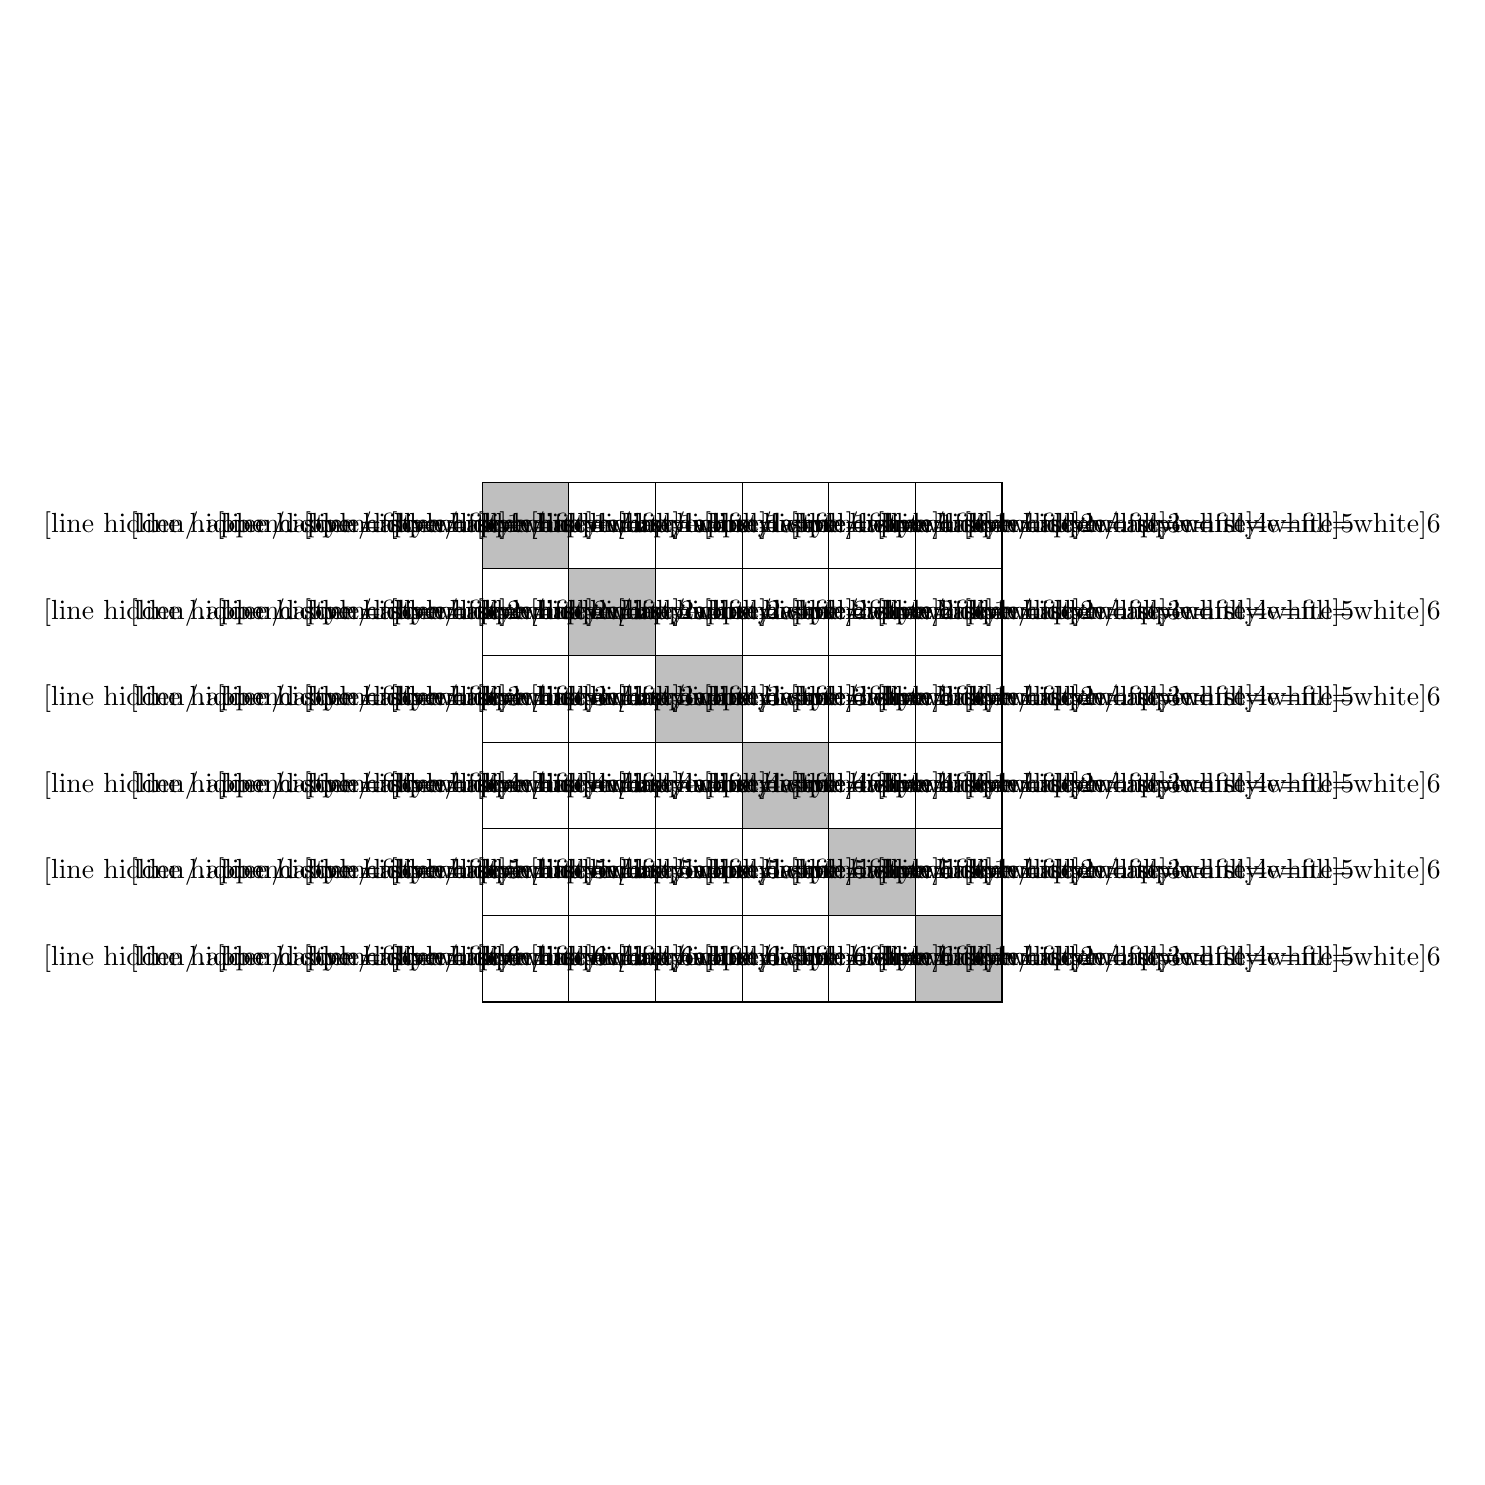
\begin{tikzpicture}[scale=1.1]
% Draw the diagonal (must do this first
\foreach \x in {1,...,6}
{
    % Make the node a circle for space reasons, but don't draw it
    \filldraw[fill=lightgray] (\x,-\x) +(-.5,-.5) rectangle ++(.5,.5);
}
% Draw the matrix
\foreach \x in {1,...,6}
{
  % Make nodes on the outside of the matrix on the right side
  % Label them with o1, o2, etc.
  \foreach \y in {1,...,6}
  {
    \draw (\x,-\y) +(-.5,-.5) rectangle ++(.5,.5);
    % Make the node a circle for space reasons, but don't draw it
    \draw (\x,-\y) node[circle, inner sep=2mm] (n\y\x) {
                                           \drawdie[line hidden/.append style={fill=white}]{\y}
                                           \drawdie[line hidden/.append style={fill=white}]{\x}
                                           }; %reverse the x and y to give the expected behaviour
  }
}
\end{tikzpicture}
\end{center}
%
Now, depending on what the interviewer meant by the question, the answer is one of the following.
\begin{enumerate}
  \item
The probability of one die being larger than the other (not caring which one) is like saying what is the probability that they are not the same.
That is everything but the diagonal,
\[
  \frac{36- 6}{36} =  \frac{30}{36} = \frac{5}{6}
  \text{.}
\]
  \item
If the interviewer wanted the probability of die $A$ being more than die $B$ then the possibilities are everything in the upper/lower triangle of the matrix (half of the answer given above),
\[
  \frac{15}{36} = \frac{5}{12}
  \text{.}
\]
\end{enumerate}

This is a great question to start with, as it shows a trick often employed by these brainteasers.
When presented with a questions like this, one might be inclined to start writing out the calculations (involving tedious sums or integrals).
However, many of these types of questions can be quickly solved by drawing a square on which you can calculate the area without doing integrals.
Other examples are the
\emph{Stick Breaking} problem (question \ref{q:stickbreak})
and
\emph{Romeo and Juliet} (question \ref{q:romeojuliet}),
which we will encounter later.

This simple example shows the importance of interview preparation.
One might think that, on the job, a rigorous solution is preferred to a back-of-the-envelope one.
One might be right, but the interviews aren't testing for job preparedness.
They are probably trying to test for several qualities, but they end up selecting the candidates who are the most prepared for brainteasers.
The format is akin to asking candidates to do a Rubik's cube and preferring the one who memorised the solution by rote and solves it in two minutes, rather than the one who takes the cube home and solves it over the course of three months without looking at the solution online.
Who would you rather have work for you?
Your answer is irrelevant.
Just know that brainteasers favour the former candidate and keep it in mind during preparation.
Use the pretty solution during the interview and leave the rigorous integrals for a Saturday night with a glass of whiskey in your study, while reflecting on the fact that people in quantitative finance are probably all brainteaser savants.
\end{answer}

\begin{answer}{bivariatenormalmax}
Sometimes there isn't a quick and easy solution, and you have to do the tedious calculations.
This question is particularly nasty since it requires some niche definitions.
Doing the whole question isn't possible in the 10 minutes you will be allocated, so the interviewer is testing how well you perform under pressure,
how you approach a difficult problem by breaking it into smaller parts,
and what notation you use.

Start solving the problem with the method that seems most appropriate to you, and try to think aloud:
``We want to evaluate an expectation, so we have to do an integral.''
Don't be afraid to ask the interviewer things like ``Do you think I'm on the right track?''
They will often offer little hints to help you along.
The last thing you want to do is get started on the wrong track and struggle with it for ten minutes while the interviewer sits there watching in silence.\footnote{During one of my interviews the interviewer started doing something on his phone while I was attempting the problem. No matter how I prodded, I couldn't get the guy interested in the interview. You win some, you lose some.}
Try to get the interviewer involved, but not to such an extent that you need your hand held.
This is something that takes practise.
For our current problem, we have to write it into something easier first,
\[
  \max(X, Y) =
  \begin{dcases*}
    Y & if $Y \geq X$\\
    X & if $X < Y$
  \text{.}
  \end{dcases*}
\]
Now we can use the Law of Total Expectation:
\index{tricks!Law of Total Expectation}
If $ A_1, A_2, A_3, \ldots, A_n$ are mutually disjoint and exhaustive, then
\[
  \E(Z) = \sum_{i=1}^{n}{
    \E(Z| A_i)P(A_i)
  }
  \text{.}
\]
You've probably never had to use it in this form before, but it comes in handy for this brainteaser.
In our case, let $Z=\max(X,Y)$, with the expectation expanded as
\begin{align*}
  \E(Z) &= \E(Z|X > Y)P(X>Y)
+          \E(Z|X \leq Y)P(X \leq Y) \\
        &= \E(X|X > Y)P(X>Y)
+          \E(Y|X \leq Y)P(X \leq Y)
  \text{.}
\end{align*}
Now, the interviewer will point out that the two terms on the right-hand side are symmetric, thus they must be the same:
\[
  \E(Z) = 2 \E(X|X > Y)P(X>Y)
  \text{.}
\]
Here, $P(X>Y) = \nicefrac{1}{2}$ and doesn't depend on $\rho$---the integration that proves this is tedious and, again, it is easier to draw a picture.
Below is a contour plot of the bivariate normal distribution with
\[
\vec{\mu}=
\begin{bmatrix}
  0    \\
  0
\end{bmatrix}
\text{ and }
\Sigma =
\begin{bmatrix}
  1    & \rho \\
  \rho & 1    \\
\end{bmatrix}
\]
for different values of $\rho$.
The contour plot is something you can quickly draw up.
Refer to the three-dimensional plots below for clarity.
\begin{center}
  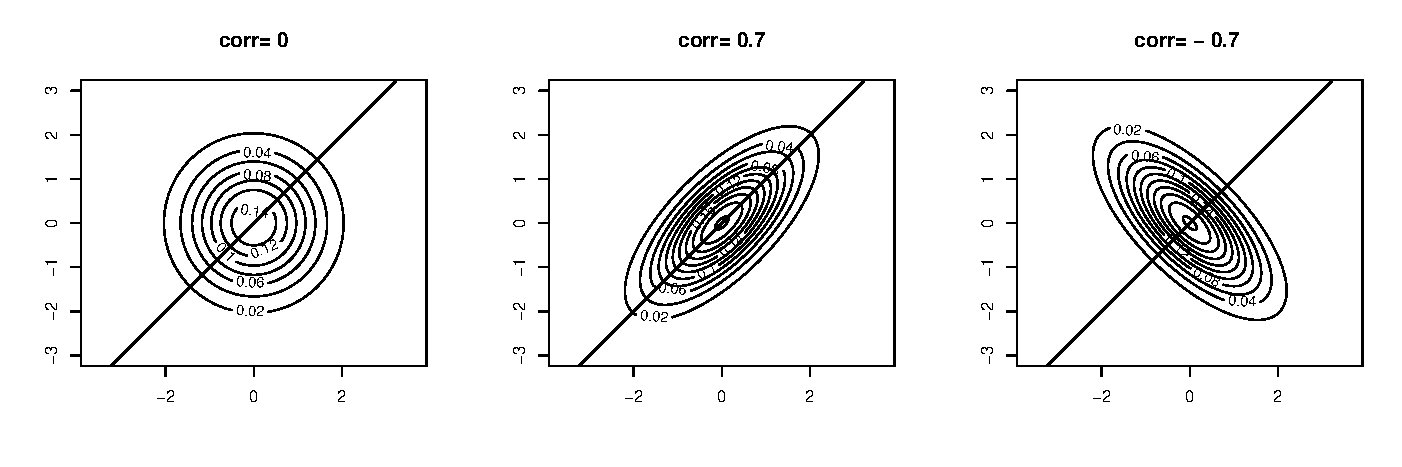
\includegraphics[width=\textwidth]{./plots/mvtnorm/mvrnorm.pdf}
  % mvrnorm.pdf: 0x0 pixel, 300dpi, 0.00x0.00 cm, bb=
  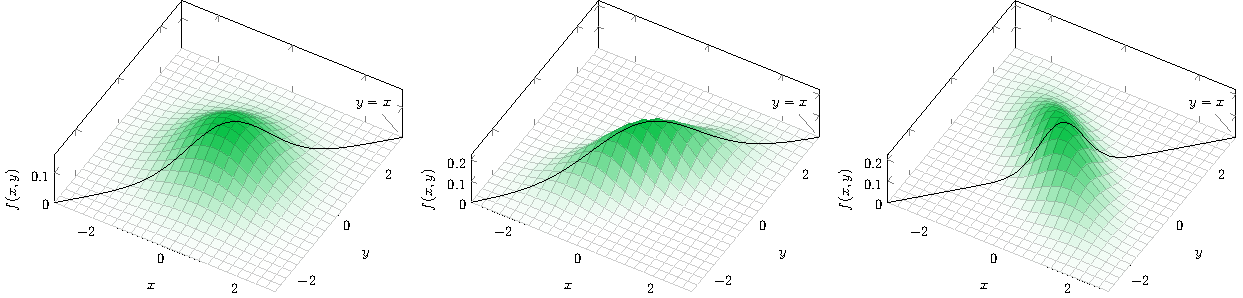
\includegraphics[width=\textwidth]{./plots/bivariatenorm/bivariatenorm.pdf}
\end{center}
The line shows $y=x$; the area under the distribution where $x>y$ will be equal to \nicefrac{1}{2} for any value of $\rho$.
Thus we have reduced the problem to
\[
\E(Z) =  \E(X|X > Y)
\]
and we just need to find a clever way to evaluate it.
If you have got this far, the interviewer will probably be convinced of your ability to solve the problem, and move on to the next question.
Some firms  ask really difficult questions, but they don't expect you to get the correct answers.
(This is especially the case with Goldman Sachs.)
They want to see how you think.
At some hedge funds I saw the opposite: they ask moderately difficult questions and snidely remark that you seem unable to do the ``simple proof'' which they pretend to know (especially silly, given that they checked the solution just before you walked in) if you don't start off on the right foot.
You win some, you lose some.

I will give the rest of the answer here for the sake of completeness, and then I will present a clever solution provided by a friend.
You will notice that the solution is complicated and requires a fair amount of textbook theory (like the properties of a truncated normal distribution, for example).
Even if you are able to recall all the required properties during an interview, doing a rigorous proof will take longer than the time allocated.
Again, the interviewer probably isn't looking for the whole proof, but rather the steps you would take along the way.

The quantity $\E(X|X > Y)$ isn't immediately recognisable.
However, if we let
\begin{align*}
W_1 &= X \\
W_2 &= X-Y
\end{align*}
and write the expectation as
\begin{align*}
\E(X|X-Y > 0) = \E(W_1|W_2 > 0)
\end{align*}
it becomes a conditional expectation of two random variables that are a linear combination of our original bivariate normal distribution.
To see this, use a matrix
\[B =
\begin{bmatrix}
  1   &  0 \\
  1   & -1 \\
  \end{bmatrix}
\]
then
\[
\begin{bmatrix}
  W_1 \\ W_2
\end{bmatrix}
=
B
  \begin{bmatrix}
  X \\ Y
  \end{bmatrix}
  =
  \begin{bmatrix}
  X \\ X-Y
  \end{bmatrix}
  \text{.}
\]
This is an affine transformation of a multivariate normal distribution, which is also multivariate normal:
\[
\begin{bmatrix}
  W_1 \\ W_2
\end{bmatrix}
=
B
\begin{bmatrix}
X \\ Y
\end{bmatrix}
\sim
\operatorname{MultivariateNormal}
\left(
B
\begin{bmatrix}
0 \\ 0
\end{bmatrix}
  ,
  B
  \begin{bmatrix}
  1      &   \rho \\
  \rho   &   1    \\
  \end{bmatrix}
  B^T
  \right)
  \text{.}
\]
Thus
\[
\begin{bmatrix}
W_1 \\ W_2
\end{bmatrix}
=
\begin{bmatrix}
X \\ X - Y
\end{bmatrix}
\sim
\operatorname{MultivariateNormal}
\left(
\begin{bmatrix}
0 \\ 0
\end{bmatrix}
,
\begin{bmatrix}
        1 &    1 -\rho \\
  1-\rho  &  2(1 - \rho)
\end{bmatrix}
  \right)
\]
and we can use the conditional properties of the multivariate normal distribution to evaluate
\begin{equation}
\label{eq:bivariatenormalmax:conditional_expecation}
\E(X|X-Y > 0)
\end{equation}
as
\begin{equation*}
\E(W_1|W_2 > 0)
\text{.}
\end{equation*}
This conditional expectation is difficult to evaluate.
In general, if we partition a $p$-dimensional multivariate normal vector
\[
\vec{x} \sim \operatorname{MultivariateNormal}(\vec{\mu}, \vec{\Sigma})
\]
into $\vec{x} = [\vec{x_1}, \vec{x_2} ]^{T}$ where
$x_1 \in \mathbb{R}^k$ and
$x_2 \in \mathbb{R}^{p-k}$ such that
\[
\begin{bmatrix}
\vec{x}_1 \\ \vec{x}_2
\end{bmatrix}
\sim
\operatorname{MultivariateNormal}
\left(
\begin{bmatrix}
\vec{\mu}_1 \\ \vec{\mu}_2
\end{bmatrix}
,
\begin{bmatrix}
\vec{\Sigma}_{11} & \vec{\Sigma}_{12} \\
\vec{\Sigma}_{21} & \vec{\Sigma}_{22} \\
\end{bmatrix}
  \right)
\]
we know from the theory of the multivariate normal distribution that
\[
  (\vec{x}_1 | \vec{x}_2 =  \vec{a})
  \sim
\operatorname{MultivariateNormal}
\left(
\vec{\mu}_1 +
\vec{\Sigma}_{12}
\vec{\Sigma}_{22}^{-1}
(\vec{a} - \vec{\mu}_2)
\, , \,
\vec{\Sigma}_{11}
-
\vec{\Sigma}_{12}
\vec{\Sigma}_{22}^{-1}
\vec{\Sigma}_{21}
  \right)
\text{.}
\]
In our example the partitioning is simple as it doesn't involve block matrices, and we have
\begin{align*}
\E(W_1|W_2 = w_2) &=  \frac{(1-\rho)}{2(1-\rho)} w_2 \\
                  &=  \frac{1}{2}w_2
\text{.}
\end{align*}
Using (somewhat liberally) the tower property of the Law of Total Expectation,
\begin{align*}
\E(X \, | \, f(Y)) &=
\E( \E(X\,|\,Y) \; | \; f(Y))
\text{,}
\end{align*}
we can write
\begin{align*}
\E(W_1|W_2 > 0 )
&=
\E( \E(  W_1| W_2) \;|\; W_2 > 0 ) \\
&= \E\left( \frac{1}{2}W_2 \; \Bigg| \; W_2>0 \right) \\
&= \frac{1}{2}\E( W_2 | W_2>0 )
\text{.}
\end{align*}
This is $\nicefrac{1}{2}$ multiplied by the expected value of a truncated normal distribution,
\begin{align}
\E(W_2|W_2 > 0)
&= 0 + \frac{ \sqrt{2( 1- \rho)} \phi(0)}{1- \Phi(0)} \label{eq:bivariatenormalmax:conditional_expecation2} \\
&=  \frac{ \sqrt{2( 1- \rho)} \frac{1}{\sqrt{2 \pi}} }{\frac{1}{2}} \nonumber \\
&=  \frac{ 2 \sqrt{ 1- \rho}  }{ \sqrt{ \pi} } \nonumber
\text{.}
\end{align}
Putting it all together we finally arrive at the answer,
\begin{align*}
\E(Z) &=  \E(X|X > Y)  \\
      &= \E(W_1|W_2 > 0 ) \\
      &= \frac{1}{2}E(W_2|W_2>0) \\
      &=  \frac{1}{2}\frac{ 2 \sqrt{ 1- \rho}  }{ \sqrt{ \pi} } \\
      &=  \sqrt{\frac{ 1- \rho  }{ \pi }}
\text{.}
\end{align*}
You can use Monte Carlo integration to convince yourself of this; I've included an R script in appendix \ref{ap:mvtnormproof} to do just that.




My friend's solution begins differently.
It uses the identity
\[
  \max(x,y) = \frac{x + y + |x-y|}{2}
  \text{.}
\]
Using this, the expectation becomes
\begin{align*}
  \E(\max(X,Y))
  &= \frac{1}{2}\E(X + Y + |X-Y|) \\
  &= \frac{1}{2}\E(|X-Y|) \qquad \text{because } \E(X) = \E(Y) = 0 \\
  &= \frac{1}{2}
  \bigg(
     \E(X-Y |X-Y > 0 ) P(X-Y > 0)  \\
  &\qquad + \E(Y-X |X-Y \leq 0 ) P(X-Y \leq 0)
  \bigg) \quad \text{total expectation} \\
  &= \frac{1}{2} 2
    \bigg(
      \E(X-Y |X-Y > 0 ) P(X-Y > 0)
    \bigg) \quad \text{symmetry} \\
  &=
    \E(X-Y |X-Y > 0 ) \frac{1}{2}
\text{.}
\end{align*}
The random variable $W_2 = X-Y$ has a $\text{normal}(0, 2(1-\rho))$ distribution.
To see this, use a matrix $B=
\begin{bmatrix}
        1 &    -1 \\
\end{bmatrix}
$ for an affine transformation as above, or consider that the sum of two random variables each from a normal distribution is itself a normal distribution, where you have to find
$\E(W_2) = \E(X-Y)$
and
$\Var(W_2) = \Var(X-Y)$.
So now we have
\begin{align*}
\E(X-Y|X-Y > 0) &=  \E(W_2|W_2 > 0)
\end{align*}
which is the same expectation we had in (\ref{eq:bivariatenormalmax:conditional_expecation2}), thus
\begin{align*}
\E(X-Y|X-Y > 0) =
 \frac{ 2 \sqrt{ 1- \rho}  }{ \sqrt{ \pi} }
\end{align*}
and
\[
\E(\max(X, Y)) = \sqrt{\frac{  1- \rho  }{  \pi }}
\text{,}
\]
corroborating our earlier answer.

\end{answer}


\begin{answer}{makematrixfrombunchofvectors}
Assuming the vectors are all of the same size, we can use
\verb+cbind()+ to bind the vectors as columns
or
\verb+rbind()+
to bind the vectors as rows.

If you get this question, you probably mentioned R \citep{RCoreTeam} on your CV, and the interviewer is testing to see whether you actually use it (rather than just having read an intro or tutorial).
Be prepared for similar questions about all the languages you mention on your CV.
\end{answer}

\begin{answer}{pythonlistreturnlast}
It returns the last item in \verb+mylist+.
This question is asked in the same spirit as the previous one.
They are probably checking whether you will confuse it with R, where
\verb+myvec[-1]+ will return everything except the first entry of the vector \verb+myvec+.
\end{answer}

\begin{answer}{cppvirtualfunctionwhy}
This is question 7.10 from \citet{JoshiQA}
and their wording is probably better than my own.
Virtual functions allow us to defer the implementation of a function.
When we define a virtual function in a base class, we don't have to specify its workings; we can do that later in the classes that inherit from it.

For instance, I might have a base class called \verb+ContinuousDistribution+ with a virtual function  called \verb+simulateRandomVariable+.
This way, I don't have to implement the function that does the simulation in the base class, I can define it for each of the distributions I implement.
You can also implement a general, inefficient function the base class and override it in the derived classes with more appropriate functions for each distribution.
The example I give is different from
\citet[question 7.10]{JoshiQA},
and I suggest you think of an example to use which is relevant to you and your background.
It is much easier to remember your own example in an interview than learning someone else's.
It also conveys actual working knowledge rather than prepared responses---whether merited or not.


The second part of the question is harder to answer and interviewers are likely to have different views.
I got asked why we need virtual functions if we can probably use function pointers and other C++ tricks to mimic their behaviour.
In truth, virtual functions aren't only used to defer implementation.
The academic answer is ``It is used to give Run Time Polymorphism,'' but  make sure you know what this means if you want to use it.
It is best explained through an example, like the one given in appendix \ref{ap:virtualfunctions}.
We can use a base-class pointer to point to a base class (Car, in the example), as well as a derived class (ElectricCar, in the example).
When we call a function using the base-class pointer, the compiler decides at run time which function to call, and in the case of a virtual function it will prefer the derived-class version.
This ability is hard to mimic without virtual functions---we would have to overload a lot of  functions outside of the classes themselves.
With virtual functions, the programmer only has to worry about specifying all the correct functions in their class, rather than also deal with an additional list of external functions to overload.

If you mentioned C++ on your CV you should be able to answer all the questions in
\citet[chap.~7]{JoshiQA}.
Study them even if you think you know the language well; it has all the important questions along with the answers \emph{as the interviewers want to hear them}.
I can also wholly suggest \citet{joshi2008cpp}, which is not only the definitive text on its subject, but also a great book on C++ design patterns in general.
At the very least, be ready to answer questions about virtual functions, polymorphism, and some design patterns in C++.
Questions about differences between Python and C++ are also popular.
\end{answer}




\clearpage
\subsection{Face-to-face, 1 hour}
\begin{question}{normalfourthmoment}
\index{questions!normal fourth moment}
Derive $\operatorname{E}(X^4)$ where $X \sim \text{Normal}\left(0, \sigma^2\right)$.
\end{question}


\begin{question}{arraymissingnumber}
\index{questions!array with missing number}
You have an unsorted array containing integers $1,2,3, \ldots, n$, but one number is missing.
Describe an algorithm to find the missing number and discuss its complexity.
\end{question}


\begin{subquestion}{arraymissingnumber:a}
Describe an algorithm assuming there are $k$ missing numbers, where $k$ is much smaller than $n$.
\end{subquestion}


\begin{subquestion}{arraymissingnumber:b}
Describe an algorithm assuming the initial array was sorted.
\end{subquestion}


\clearpage
\begin{answer}{normalfourthmoment}
Let's do some integration and see where we end up.
We need to derive the fourth moment,
\begin{align}
\E(X^4)
&= \int_{-\infty}^{\infty}{
          x^4
          f(x)
          dx} \nonumber \\
&= \int_{-\infty}^{\infty}{
          x^4
          \frac{1}{\sqrt{2 \pi} \sigma }
          \exp{\left( -\frac{x^2}{2\sigma^2}  \right)}
          dx}
\label{eq:normalfourthmoment:integraltosolve}
\text{.}
\end{align}
There doesn't appear to be a quick way to do this integral, so we will have to use integration by parts:
\[
\int_{-\infty}^{\infty}{ u dv }
=
uv\Big\vert_{x=-\infty}^{x=\infty} - \int_{-\infty}^{\infty}{ v du }
\text{.}
\]
We will require some trial and error to determine the best way to rewrite
(\ref{eq:normalfourthmoment:integraltosolve}) in order to choose $u$ and $v$.
Be sure to tell the interviewer what you are doing while you are writing out the formula for integration by parts, and mention you are trying to find the best candidates for $u$ and $v$.
The only candidate that gives us something \emph{easier} to deal with after integration by parts is
\begin{align*}
\E(X^4)
&=
          \frac{1}{\sqrt{2 \pi} \sigma }
          \int_{-\infty}^{\infty}{
          x^3
          \;
          x
          \exp{\left( -\frac{x^2}{2\sigma^2}  \right)}
          dx}
\text{.}
\end{align*}
Then we have
\begin{align*}
u   &= x^3      \\
dv  &=
        x
        \exp{\left( -\frac{x^2 }{2\sigma^2} \right)}
        dx
        \\
%
du  &= 3 x^2 dx \\
v   &=
       - \sigma^2
        \exp{\left( -\frac{x^2}{2\sigma^2}  \right)}
\end{align*}
giving
\begin{equation}
\begin{aligned}
\label{eq:fourthmoment:nearlythere}
\frac{1}{\sqrt{2 \pi} \sigma }
\int\limits_{-\infty}^{\infty}{
  x^3
  \;
  x \exp{\left( -\frac{x^2}{2\sigma^2}  \right)}
}
=
&-\frac{1}{\sqrt{2 \pi} \sigma }
x^3
\sigma^2
\exp{\left( -\frac{x^2}{2\sigma^2}  \right)} \bigg|_{x=-\infty}^{x=\infty}
\\
&+
\frac{1}{\sqrt{2 \pi} \sigma }
\int\limits_{-\infty}^{\infty}{
  \sigma^2
  \exp{\left( -\frac{x^2}{2\sigma^2}   \right)}
 3 x^2
  dx
}
\text{.}
\end{aligned}
\end{equation}
The first term on the right hand side is equal to zero.
We can use L'Hôpital's rule to prove it.%
\footnote{But be wary:
I once got reprimanded during an interview at a hipster hedge fund for suggesting
L'Hôpital's rule as a solution to a problem that had the form $\nicefrac{\infty}{\infty}$.
The interviewer had never heard of L'Hôpital, and snidely enquired whether it was some sort of food.
I was impressed that someone managed to graduate with a physics degree without ever encountering L'Hôpital.
The interviewer must have been great at brainteasers to get hired.}
We need to apply the rule three times:
\begin{equation}
\label{eq:fourthmoment:lhopital}
\begin{aligned}
\lim_{x \rightarrow \infty}
-x^3
\sigma^2
\exp{\left( -\frac{1}{2\sigma^2} x^2 \right)}
&=
\lim_{x \rightarrow \infty}
\frac{-x^3 \sigma^2 }{ \exp{\left( \frac{1}{2\sigma^2} x^2 \right)} }
\quad\text{rewrite as fraction}
\\
&=
\lim_{x \rightarrow \infty}
\frac{
  - 3 \sigma^{2} x^{2}
  }{
  \quad \frac{x}{\sigma^{2}} \exp{\left(\frac{x^{2}}{2 \sigma^{2}}\right)}
  }
\quad\text{L'Hôpital 1}
\\
&=
\lim_{x \rightarrow \infty}
\frac{ - 6 \sigma^{2} x }{
\frac{1 }{\sigma^{2}} \left(1 + \frac{x^{2}}{\sigma^{2}}\right)
\exp{\left(\frac{x^{2}}{2 \sigma^{2}}\right)}
}
\quad\text{L'Hôpital 2}
\\
&=
\lim_{x \rightarrow \infty}
\frac{ - 6 \sigma^{2} }{
\frac{x}{\sigma^{4}} \left(3 + \frac{x^{2}}{\sigma^{2}}\right)
\exp{\left(\frac{x^{2}}{2 \sigma^{2}}\right)}
}
\quad\text{L'Hôpital 3}
\\
&= 0
\end{aligned}
\end{equation}
and the same is true for
${x \rightarrow -\infty}$.
While I include the elaborate calculations above, you don't have to, because it is clear that the denominator will always include a term involving
\[
\exp{\left(\frac{x^{2}}{2 \sigma^{2}}\right)}
\]
while the nominator will eventually become zero after enough differentiation.
So now (\ref{eq:fourthmoment:nearlythere}) becomes
\begin{align*}
\frac{1}{\sqrt{2 \pi} \sigma }
\int\limits_{-\infty}^{\infty}{
  x^4
  \exp{\left( -\frac{x^2}{2\sigma^2}  \right)}
  dx
}
&=
3 \sigma^2
\frac{1}{\sqrt{2 \pi} \sigma }
\int\limits_{-\infty}^{\infty}{
  x^2
  \exp{\left( -\frac{x^2}{2\sigma^2}  \right)}
  dx
}
\text{.}
\end{align*}
The right hand side is equal to $3\sigma^2$ multiplied by the second moment of a normal distribution with mean zero and standard deviation $\sigma$.
Recall that if $X \sim \text{Normal}(\mu, \sigma^2)$ we have
\begin{align*}
  \Var(X) &= \E(X^2) - \E(X)^2 \\
\sigma^2  &= \E(X^2) - \mu^2
\end{align*}
meaning
$ \E(X^2) = \sigma^2 $
when
$\mu=0$.
Thus the fourth moment of
$X \sim \text{Normal}\left(0, \sigma^2\right)$ is
\begin{align*}
\E(X^4)
&=
3 \sigma^2 \E(X^2)
\\&=
3 \sigma^4
\text{.}
\end{align*}
This was a very long journey to arrive at the answer, and doing the integration may not have been the best approach.
This approach does, however, allow you to exhibit your integration prowess, which may hurt or help you depending on how the interviewer feels.
In my case, I wasn't able to arrive at the right answer, but when I reached  (\ref{eq:fourthmoment:nearlythere}) the interviewer said ``there, now we have something familiar'' (referring to the second moment) and went on to the next question.
A better approach might have been to use the Moment Generating Function of the normal distribution,
\begin{align*}
  M(t) =
  e^{\mu t}
  e^{\frac{1}{2}\sigma^2 t^2}
  \text{.}
\end{align*}
Then we can calculate any moment using
\[
E \left( X^n \right) = M_X^{(n)}(0) = \left. \frac{d^n M_X (t)}{dt^n}\right|_{t=0}
\]
where $M_X^{(n)}(t)$ is the $n$th derivative of the function $M(t)$.
For our case where $\mu=0$,
\begin{align*}
  M_X(t) &=
  e^{\frac{1}{2}\sigma^2 t^2}\\
M_X^{(1)}(t) &=
\sigma^{2} t e^{\frac{\sigma^{2} t^{2}}{2}}
\\
M_X^{(2)}(t) &=
\sigma^{2} \left(\sigma^{2} t^{2} + 1\right) e^{\frac{\sigma^{2} t^{2}}{2}}
\\
M_X^{(3)}(t) &=
\sigma^{4} t \left(\sigma^{2} t^{2} + 3\right) e^{\frac{\sigma^{2} t^{2}}{2}}
\\
M_X^{(4)}(t) &=
\sigma^{4} \left(\sigma^{4} t^{4} + 6 \sigma^{2} t^{2} + 3\right) e^{\frac{\sigma^{2} t^{2}}{2}}
\\
M_X^{(4)}(0) &=
3\sigma^{4}
\text{.}
\end{align*}
Still tedious, but perhaps less so than the integration.%
\footnote{I used Sympy by \citet{Sympy} to generate these, as well as all the differentiation for in (\ref{eq:fourthmoment:lhopital}).}
Of course, you could just learn the moments of the normal distribution by heart, but I don't think that's what interviewers want---they want to see some mathematics.
In my case, the interviewer also asked me what the fourth moment meant.
I didn't understand, but they probably wanted me to mention the kurtosis, which is a measure of the ``tailedness'' of a distribution.\
The fourth moment is used to measure kurtosis,
the third moment is related to the skewness,
the second moment to the variance, and the first moment is the mean.


In my experience, interviewers from investment banks love questions about the normal distribution.
This might be in response to interview solution manuals like
\citet{HeardOnTheStreet} and \citet{JoshiQA},
and the fact that they don't contain many questions on the theory of the normal distribution.
Perhaps there is a book called ``Interesting Proofs about the Normal Distribution'' doing the rounds at the banks, or maybe there are internal study groups who meet regularly to make and solve brainteasers about the normal distribution.
Whatever it is, I cannot guarantee that these questions will remain popular.
I nonetheless recommend that you know the normal distribution well---not only because it might help you during interviews, but also because it is, by now, an overused distribution that you are sure to encounter in practice.
\end{answer}

\begin{answer}{arraymissingnumber}
For the case of one missing number, we know the sum is supposed to be
\[
  \frac{n (n+1) }{2}
  \text{,}
\]
so we can calculate the sum of the $n$ numbers, and the difference will be the missing number.
The computational complexity of this is $O(n)$, since we need to add the $n-1$ numbers.
\end{answer}
\begin{subanswer}{arraymissingnumber:a}
This is a little harder to figure out.
\index{tricks!start with simplest case}
If you struggle, think about the case with two missing numbers.
Then think of three.
This step-by-step thinking should help you to arrive at the general case.
For many brainteasers, it helps to start with the case of $n=1$ and then generalise, as discussed in appendix \ref{ap:tricks}.
The general solution to this question is similar to the case of one missing number.
You have $n-k$ numbers $x_1, x_2, x_3, \ldots , x_{n-k}$.
To find the $k$ missing values, calculate
\begin{align*}
& \sum_{i=1}^{n-k}{ x_i   } \\
& \sum_{i=1}^{n-k}{ x_i^2 } \\
& \sum_{i=1}^{n-k}{ x_i^3 } \\
& \quad\vdots \\
& \sum_{i=1}^{n-k}{ x_i^k }
\end{align*}
and compare these with their theoretical values.
The result is a system of $k$ equations to solve, with $k$ unknowns.
The answers represent the missing numbers.
For instance, say we have three missing numbers, $m_1, m_2$, and $m_3$, then we can set up the following equations,
\begin{align*}
 \overbrace{\frac{n(n+1)}{2}}^{ \text{Theoretical} \atop \text{value} }
 &=
 \sum_{i=1}^{n-3}{ x_i }
+  m_1 + m_2 + m_3
\\
 \frac{n(n+1)(2n + 1)}{6}
 &=
 \sum_{i=1}^{n-3}{ x_i^2 }
+ m_1^2 + m_2^2 + m_3^2
\\
 \frac{n^2(n+1)^2}{4}
 &=
 \sum_{i=1}^{n-3}{ x_i^3 }
+ m_1^3 + m_2^3 + m_3^3
\text{.}
\end{align*}
We have three equations, and three unknowns.
You will probably have to solve this numerically, possibly by doing an exhaustive search over the integers from $1$ to $n$.
For the theoretical values, you can use Faulhaber's formula:
\[
  \sum_{k=1}^{n}{k^p} = \frac{1}{p+1} \sum_{j=0}^{p}{ (-1)^j \binom{p+1}{j} B_j n^{p+1-j} }
\]
where $B_j$ represents the Bernoulli numbers, or you can calculate them numerically.


\end{subanswer}




\begin{subanswer}{arraymissingnumber:b}
Finding one missing number in a sorted array is a trivial exercise.
We simply check that the array starts at one, then go through it checking that each number is one more than the previous one.
Any gaps represent missing numbers.
The complexity of this is $O(n)$, as we have to go through each value in the array.
This is the same complexity as the problem with one missing number in an unsorted array, which is suspicious; knowing that the array is sorted gives much more information.
Of course, we can do better.
We can check the number in the middle of the array against the expected one and then we know whether the missing value is in the top or bottom half of the array.
Repeat until we find the offending value.
This approach is known as binary search and has complexity of $O(\log_2(n))$.
\end{subanswer}



\clearpage
\subsection{Face-to-face, 1 hour}
\begin{question}{normalestimatorssamplingdistribution}
\index{questions!normal estimators}
Suppose
$Y \sim \text{Normal}(\mu, \sigma^2)$.
Now, $10^6$ people each draw 1000 samples from this distribution.
Let $i$ denote the $i$th person.
Each person estimates the parameters of the normal distribution
$\hat{\mu}_i$
and
$\hat{\sigma}^2_i$
using their samples
$Y_1, Y_2, \ldots , Y_{1000}$.
How should they do this?
If you draw a histogram of the $10^6$ estimates of
$\hat{\mu}_i$ and $\hat{\sigma}^2_i$, what would their distributions be?
How would you prove the exact sampling distribution of $\hat{\sigma}^2_i$?
\end{question}


\begin{question}{derivativeofinverse}
\index{questions!derivative of inverse}
If we have  $g'(x)$,
what can you say about $\frac{d}{dx} g^{-1}(x)$?
\end{question}

\clearpage
\begin{answer}{normalestimatorssamplingdistribution}
This is a question about sampling theory in the frequentist sense.
If you have an estimator for the parameter, and you draw repeated samples from the population, what will the distribution of the estimator be?
Note that the question isn't Bayesian, since you aren't assuming random parameters, but merely that the estimator will have a distribution due to the random sampling of the values it depends on.
The right way to estimate the parameters using the samples are through the sample mean and variance,
\begin{align*}
  \tilde{\mu}_i &= \frac{1}{n}\sum_{j=1}^{n}{y_{ij}} \\
  \tilde{\sigma}_i &=
 \sqrt{ \frac{1}{n-1} \sum_{j=1}^{n}{(y_{ij} - \tilde{\mu}_i)^2} }
 \text{.}
\end{align*}
If you draw histograms of these values, the distribution of the
$\tilde{\mu}_i$
will be normal,
because it is the sum of normal random variables $y_{ij}$ and thus also normal.
The distribution of the
$\tilde{\sigma}_i$
will be chi-squared, because it is the sum of a bunch of squared normal random variables.
The way to prove this is to use the formula for random variable transformation.
If $Z = g(X)$
then
\[
  f_Z(x) =  f_X( g^{-1}(x) )\left| \frac{d}{dx} g^{-1}(x) \right|
\]
where
$f_Z(x)$ is the pdf of $Z$ and
$f_X(x)$ is the pdf of $X$.
When I wrote this down, my interviewer
checked his notes and said
``No, that is wrong, you have to use the following formula'' and produced
\[
  f_Z(z) =  f_X( g^{-1}(z) )\left| \frac{d}{dz} g^{-1}(z) \right|
  \text{.}
\]
Then he asked me to derive it to make sure I understood where it came from.
Here is the derivation:
\begin{align*}
  F_Z(x)
  &=  P(Z < x) \\
  &=  P(g(X) < x) \\
  &=  P(X < g^{-1}(x)) \\
  &=  P(X < g^{-1}(x)) \\
  &=  F_X( g^{-1}(x) ) \\
  f_Z(x) &=  f_X( g^{-1}(x) )\left| \frac{d}{dx} g^{-1}(x) \right|
  \text{.}
\end{align*}
Notice that I used $x$ in my derivation, not $z$.
The interviewer nodded and moved on to the next question.
\end{answer}

\begin{answer}{derivativeofinverse}
  This is a question about the relationship between the derivative and the inverse of a function.
  The answer is simple, if you start correctly.
  I didn't, so I struggled with it, and after using $x$ instead of $z$ in the previous derivation                                       probably didn't leave a good impression.
  I produce the correct answer here,
\begin{align*}
  x &= x \\
  g(g^{-1}(x)) &= x \\
 \frac{d}{dx} g(g^{-1}(x)) &= \frac{d}{dx} x \\
  g'(g^{-1}(x))   \frac{d}{dx} g^{-1}(x) &= 1  \qquad (\text{chain rule})\\
 \frac{d}{dx} g^{-1}(x) &= \frac{1}{g'(g^{-1}(x))}
    \text{.}
\end{align*}
The crux is knowing to start with the first two lines, and to differentiate on both sides.
If you try solving this with integrals, as I did, you are going to have a bad time.
\end{answer}



\clearpage
\subsection{Phone interview, 45 minutes}
\begin{question}{coin100flipsgamble}
\index{questions!coin flip gamble}
You are presented with the following gamble: you flip 100 fair coins.
If 60 or more land on heads, you win \pounds 10; you win nothing on all other outcomes.
Should you play this game for \pounds 1?
\end{question}

\begin{question}{iszerocorrelationindependent}
\index{questions!correlation and dependence}
You have $X \sim \text{Normal}(0,1)$ and $Y \sim \text{Normal}(0,1)$.
If the correlation coefficient is $\rho_{XY}=0$, are $X$ and $Y$ independent?
\end{question}


\begin{subquestion}{iszerocorrelationindependentexamples}
\index{questions!correlation and dependence}
Give some examples where $X$ and $Y$ are in fact dependent, but where the above still holds.
\end{subquestion}

\clearpage
\begin{answer}{coin100flipsgamble}
This can be solved by using the Central Limit Theorem, or the normal approximation to the binomial distribution.
\index{tricks!Central Limit Theorem}
You have
\begin{align*}
  Y \sim \text{Binomial}(p=0.5, n=100)
\end{align*}
and for large $n$ you can approximate the binomial distribution through the normal distribution,
\begin{align*}
  Y &\stackrel{\sim}{\text{\tiny approx}}  \text{Normal}(np, np(1-p))
  \text{.}
\end{align*}
The values of $n$ and $p$ in the problem give
\begin{align*}
  np      &= 100\left(\nicefrac{1}{2}\right)    = 50\\
  np(1-p) &= 100\left(\nicefrac{1}{2}\right)^2  = 25
  \text{,}
\end{align*}
resulting in
\begin{align*}
  Y & \sim
  \text{Normal}\left( 50, (5)^2 \right)
  \text{.}
\end{align*}
In order to evaluate whether the gamble is worthwhile you have to calculate its expected return:
\begin{align*}
  \E(\text{Gamble}) &= -1 + (10)P(\text{Win})  + (0)P(\text{Lose}) \\
                    &= -1 + (10)P(Y>60)
                    \text{.}
\end{align*}
Given that you are in an interview, you need to evaluate $P(Y>60)$ without a calculator.
\index{tricks!normal probabilities in your head}
With the normal distribution, approximately 95\% of the data lies within two standard deviations of the mean.
For the current problem, two standard deviations from the mean is conveniently located at 60, as the following graph indicates:
\begin{center}
  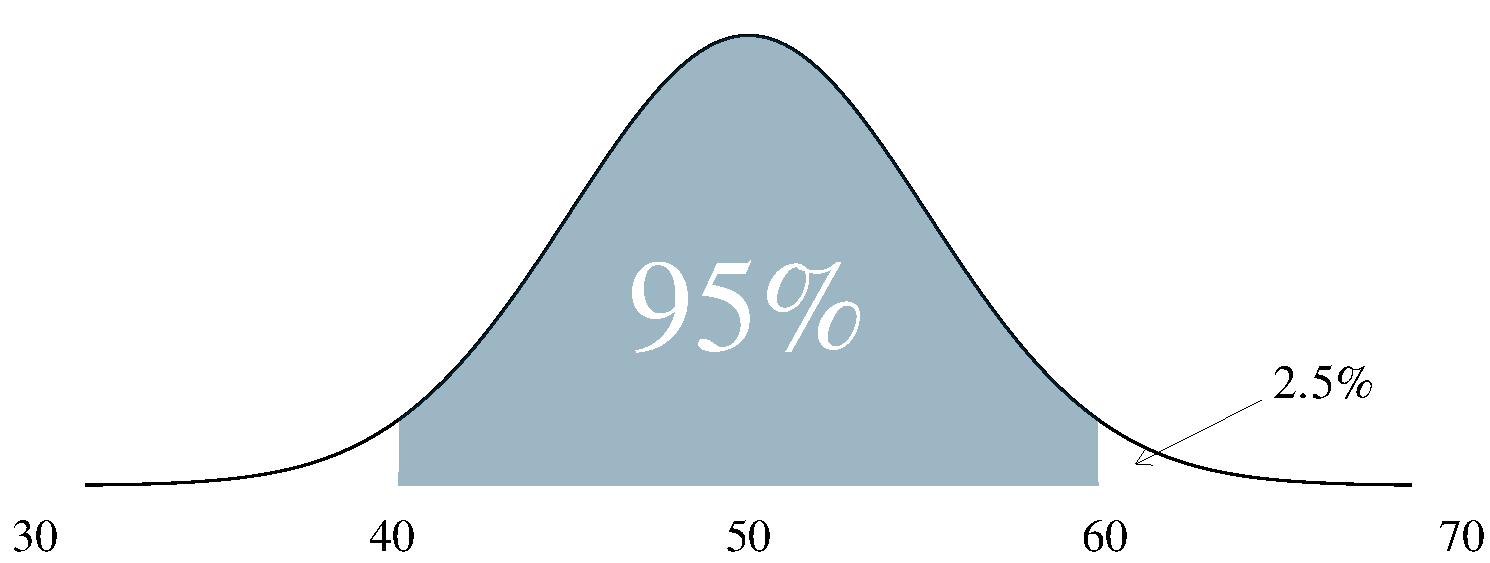
\includegraphics[width=0.8\textwidth]{./plots/prettynorm/prettynorm.pdf}
\end{center}
The probability of interest is $P(Y>60 = 0.025)$ and thus the expected value of the gamble is
\[
  \E(\text{Gamble}) = -1 + (10)(0.025) = -1 + 0.25 = -0.75
  \text{.}
\]
On average you lose 75 pence for playing the game so it is not worthwhile.
The fair price, denoted $\pounds_{\text{fair}}$, occurs where the gamble breaks even:
\begin{align*}
  \E(\text{Gamble})     &=  0    \\
  \pounds_{\text{fair}} - 0.25 &=  0    \\
  \pounds_{\text{fair}}        &=  0.25
\end{align*}
and this is the highest price at which a
rational and risk-neutral person should start agreeing to play.
The assumptions of rationality and risk neutrality are very important.
If a billionaire gets immeasurable physical pleasure from engaging in risky gambles---and therefore is not risk neutral---the rational course of action is probably to spend all of their excess money on unfair gambles.
Conversely, risk-neutral people might not always act rationally.

\end{answer}

\begin{answer}{iszerocorrelationindependent}
No.
Correlation only measures linear dependence.
They could have a non-linear dependence.
See the next question for an example.
\end{answer}

\begin{subanswer}{iszerocorrelationindependentexamples}
Let $Z$ have the probability mass function
\begin{align*}
p(z) =
\begin{cases}
  0.5 & \text{ if } z = -1 \\
  0.5 & \text{ if } z = 1
\end{cases}
\end{align*}
or equivalently
\begin{align*}
P(Z = -1) &= 0.5  \\
P(Z =  1) &= 0.5
\text{.}
\end{align*}
Let $X \sim \text{Normal}(0,1)$
and
$Y = ZX$.
Derive the distribution of $Y$ using its cumulative distribution function:
\begin{align*}
P(Y<x) &=
P( ZX<x| Z = 1)P(Z=1) +
P( ZX<x| Z = -1)P(Z=-1) \\
&=
P( X<x)(0.5) + P(-X<x)(0.5) \\
&=  (0.5)( P( X<x) + P(X \geq -x)) \\
&=  (0.5)( P( X<x) + P(X < x)) \quad \text{symmetry} \\
&=   P(X < x)
\end{align*}
meaning $Y$ has the same distribution as $X$.
Now, check whether $\rho=0$,
\begin{align*}
\rho
&= \frac{\Cov(X,Y)}{\sigma_X \sigma_Y}  \\
&= \Cov(X,Y) \\
&= \Cov(X, ZX) \\
&= \E(XZX) - \E(X) \E(ZX)  \\
&= \E(X^2 Z) - \E(X) \E(ZX)  \\
&= \E(X^2) \E(Z) - \E(X)\E(Z)\E(X)   \quad \text{independence} \\
&=  0                                \quad \text{since } E(Z)=0
\text{.}
\end{align*}
You have successfully constructed a situation where
there is a clearly defined dependence between $Y$ and $X$, but
they are both distributed $\text{Normal}(0,1)$ with correlation coefficient
$\rho = 0$.
\end{subanswer}



\clearpage
\subsection{Online pair-programming interview, 60 minutes}
\begin{question}{twournsallocateballs}
\index{questions!urns and balls}
You have two urns, five red balls, and five blue balls.
You can distribute the balls into the urns any way you like, but each urn must have at least one ball in it.
I will choose one urn at random ($p=0.5$) and then draw one ball from it.
If the ball is blue, you win.
How should you distribute the balls to maximise your probability of winning?
Log into this pair-programming website and use Python or C++ to solve the problem while I watch.
\end{question}

\clearpage
\begin{answer}{twournsallocateballs}
Let $B_1$ be the number of blue balls in urn 1, and
$R_1$ be the number of red balls in urn 1.
Then
\begin{equation}
\label{eq:urns:crux}
\begin{aligned}
 P(\text{Win})
 &=
  \frac{1}{2}
  \left(
  \frac{B_1}{B_1 + R_1}
  \right)
  +
  \frac{1}{2}
  \left(
  \frac{B_2}{B_2 + R_2}
  \right)
  \\
 &=
  \frac{1}{2}
  \left(
  \frac{B_1}{B_1 + R_1}
  \right)
  +
  \frac{1}{2}
  \left(
  \frac{5 - B_1}{10 - (B_1 +R_1)}
  \right)
  \text{.}
\end{aligned}
\end{equation}
We need to find the values for $B_1$ and $R_1$ that minimises this.
The interviewer wanted me to explain how I would solve the question, and then we went into an online pair-programming room, where we found the solution in Python using ``brute force'': exploration of the whole solution space.
We can also find the solution by some reasoning.
If we wanted to maximise the probability of winning in the one bucket, we could put just one red ball in it, and no blue balls.
Then the probability of winning becomes
\begin{equation*}
\begin{aligned}
 P(\text{Win})
 &=
  \frac{1}{2}
  \left(
  1
  \right)
  +
  \frac{1}{2}
  \left(
  \frac{4}{9}
  \right)
  \\
 &=
  \frac{1}{2}
  \left(
  \frac{13}{9}
  \right)
  \\
 &=
  \left(
  \frac{13}{18}
  \right)
  \text{,}
\end{aligned}
\end{equation*}
which is near three quarters. In fact, this is a strategy that will have a winning probability approaching $\nicefrac{3}{4}$ as the number of balls approach infinity.
\begin{align*}
  \frac{1}{2}
  \left(
  1
  \right)
  +
  \frac{1}{2}
  \left(
  \frac{\frac{N}{2} - 1}{N - 1}
  \right)
  &=
  \frac{1}{2}
  \left(
  \frac{ N-1 + \left( \frac{N}{2} - 1 \right) }{N - 1}
  \right)
  \\
  &=
  \frac{1}{4}
  \left(
  \frac{ 2N-2 +  N - 2  }{N - 1}
  \right)
  \\
  &=
  \frac{1}{4}
  \left(
  \frac{ 3N - 4  }{N - 1}
  \right)
  \text{.}
\end{align*}

The hardest part about this question is coming up with (\ref{eq:urns:crux}).
Try and understand it well enough to derive it yourself.
When I did it during the interview, I started with a notation that made the problem much harder than it is (by having variables for the total number of balls in each of the urns as well).
You have to start somewhere, and my first attempt set me off on the wrong path,
but the interviewer was interested in the approach and asked me to continue with it.
I felt that the interview went pretty well, but afterwards I received feedback that the interviewer wanted me to ``intuit'' the answer, rather than solve it using mathematical reasoning.
In the past (especially with the \emph{Air Force One} question in section \ref{q:airforceone}), I was told the opposite: Use mathematics to solve the question, not intuition and logical reasoning.
You win some, you lose some.

Online pair-programming interviews are becoming more prevalent with banks betting on automation and competing for programming talent.
They usually take two forms.
The first is similar to the above, asking you to solve mathematical problem numerically.
For instance, an on-site exam once asked me to write code, by hand, to numerically solve the \emph{Stick Breaking} problem from section \ref{subsec:stickbreaking}.
The second form is that of tech-company interviews.
That is, programming questions you can expect to get at Google and Facebook, usually involving algorithms and data structures.
It is worthwhile to review some of them.
Good websites to practice and find examples are
\url{https://www.hackerrank.com/} and
\url{https://www.codewars.com/}.
Questions about sorting algorithms (see question \ref{q:arrayofintegersfindduplicate}) used to be a favourite, but interviewers have broadened their horizons in recent years.
Look for problems involving string manipulation (finding anagrams or longest substrings) like question \ref{q:pythonanagrams}.
Other examples I've encountered are question
\ref{q:davidbeckhamparty} and the \emph{Friend Circle} problem:
``A friend circle is any group of people connected by mutual acquaintances. Given an adjacency matrix of $N$ people, write code to count the number of friend circles.''
These last two examples come from graph theory, which is a well-known source of difficult tech-interview questions.
\index{Graph theory}


\end{answer}



\clearpage
\subsection{Phone interview, 45 minutes}
\begin{question}{judgescorrectverdict}
\index{questions!three judges}

There are three judges in a court, who have the following probabilities of reaching the correct verdict:
\begin{center}
\begin{tabular}{ccc}
Judge 1 & Judge 2 & Judge 3 \\
$p$ &
$p$ &
$\nicefrac{1}{2}$ \\
\end{tabular}
\end{center}
A verdict is only decided if at least two of the judges agree.
What is the probability of the court reaching the correct verdict?
\end{question}


\begin{question}{regressiontheory1}
\index{questions!regression theory}
Suppose you wanted to model $Y$ using $X$, and you decided to use the linear regression:
\[
  Y = X \beta + \varepsilon
  \text{.}
\]
What assumptions are being made?
How would you find $\beta$?
What tests can be done on $\beta$ afterwards?
\end{question}


\begin{question}{bayeslawdisease}
\index{questions!Bayes' law}
One percent of people in the world have a given disease,
the test for which is imperfect.
The test has an 80\% chance of showing positive if you have the disease, but if you do not have the disease,
there is a 10\% chance of showing a false positive.
What is the probability that you actually have the disease if your test results are positive?
\end{question}

\clearpage
\begin{answer}{judgescorrectverdict}
The court reaches the correct verdict if either two or three judges are correct.
We will have to write out all the possibilities.
One might think the solution is $1 - P(\text{All three wrong})$, but this ignores the scenario in which one judge is correct and the other two are wrong.
We have to write out all the possible combinations.
\begin{align*}
  P(\text{Three correct})  &= p p  (\nicefrac{1}{2}) \\
  P( \text{Two correct} ) &=
     p         p     (1-\nicefrac{1}{2}) +
     p       (1-p)   (\nicefrac{1}{2}) +
   (1-p)       p     (\nicefrac{1}{2}) \\
  &= p^2 - (\nicefrac{1}{2})p^2 + p-p^2 \\
  &= p - (\nicefrac{1}{2})p^2  \\
   P(\text{Correct verdict reached})
  &=
   P(\text{Two or three correct}) \\
  &= (\nicefrac{1}{2})p^2   + p - (\nicefrac{1}{2})p^2  \\
  &=  p
  \text{.}
\end{align*}
Note that you cannot use the binomial coefficients,
$\binom{3}{3}$
and
$\binom{3}{2}$,
as the judges don't all have the same $p$.
\end{answer}

\begin{answer}{regressiontheory1}
Questions about regression come up time and time again, yet it isn't discussed in any of the classic interview texts.
Therefore, this text includes the relevant regression theory for interviews in section \ref{sec:regressiontheory}, as well as a crib sheet to use during phone interviews in
appendix \ref{ap:cribsheet}.
\end{answer}

\begin{answer}{bayeslawdisease}
Bayes' law questions are extremely common, both in phone and face-to-face interviews.
The hardest part is turning the words into their respective conditional probabilities.
Start with what you want---the probability that you actually have the disease if your rest results are positive.
Put differently, $P(D_\text{yes}|\text{Test}_+)$, where
$D_\text{yes}$ means you have the disease,
$D_\text{no}$ means you are disease-free,
and
$\text{Test}_+$ or
$\text{Test}_-$ indicates the result of your test.
Using Bayes' law, re-express this as
\begin{align*}
P(D_\text{yes}|\text{Test}_+)
&=
\frac{
  P(
    \text{Test}_+
  |
    D_\text{yes}
  )
  P(
    D_\text{yes}
   )
}
{
  P(
    \text{Test}_+
  |
    D_\text{yes}
  )
  P(
    D_\text{yes}
   )
   +
  P(
    \text{Test}_+
  |
    D_\text{no}
  )
  P(
    D_\text{no}
   )
}
\text{.}
\end{align*}

Now, consider the information the interviewer gave, and hope that you have all the bits you need. (This doesn't always happen, and it can either indicate that you have some more work to do, or that the interviewer got the question wrong.)
``One percent of people in the world have this disease.''
\begin{align*}
  P( D_\text{yes} ) & = 0.01 \\
  P( D_\text{no} ) & = 0.99
  \text{.}
\end{align*}
``The test has an 80\% chance of showing positive if you have the disease,''
\[
  P( \text{Test}_+ | D_\text{yes} ) = 0.8
  \text{,}
\]
``\ldots if you do not have the disease,
there is a 10\% chance of showing a false positive.''
\[
  P( \text{Test}_+ | D_\text{no} ) = 0.1
  \text{.}
\]
Putting it all together yields
\begin{align*}
P(D_\text{yes}|\text{Test}_+)
&= \frac{ (0.8)(0.01) }{ (0.8)(0.01) + (0.1)(0.99)  }
\text{.}
\end{align*}
You need an easy way to evaluate this without a calculator, so factorise it as
\begin{align*}
\frac{ (0.8)(0.01) }{ (0.8)(0.01) + (0.1)(0.99)  }
&= \frac{ (8)(1) }{ (8)(1) + (1)(99)  } \left( \frac{1000}{1000}  \right) \\
&= \frac{8}{107}
\end{align*}
and the denominator is a prime number so you can't simplify further.
Thus, the answer is a bit less than 8\%.
(The exact answer is $0.07476636$.)

You can represent the situation in a picture to get an intuitive understanding.
In the unit square below, the shaded area represents everyone who tested positive for the disease.
The people in the little square on the bottom left (which is 1\% of the square's area) are the ones who actually have the disease.
If you tested positive, you fall in the shaded area.
The question is asking ``given that you fall somewhere in the shaded area, what is the probability that you are also in the little square with people who have the disease.''
\begin{center}

\begin{tikzpicture}[scale=0.08]
\draw (0,0) -- (0,100)     -- (100,100) -- (100,0) -- (0,0);
\draw (0,10) -- (10,10) -- (10, 0);
\filldraw[pattern=crosshatch dots, pattern color=lightgray]
(0,100)     -- (99,100)  --
(99, 90)   -- (0,90) --
(0,100);
\filldraw[pattern=crosshatch dots, pattern color=lightgray]
(0,10)     -- (8,10)  --
(8, 0)   -- (0,0) --
(0,10);
\node at (50,50)  {No Disease};
\node at (0,5) [anchor=east] {Disease};
\end{tikzpicture}

\end{center}
As a fraction, that is
\begin{align*}
\frac{ \text{Small shaded area} }{ \text{Small shaded area}+\text{Large shaded area} }
&= \frac{ (0.8)(0.01) }{ (0.8)(0.01) + (0.1)(0.99)  }
\end{align*}
which is the same as before.
The picture reveals the nuances in Bayes' law questions and the reason for their unintuitive answers.
There is a low prevalence of the disease, together with a high false-positive rate.
Ten percent might not seem high for a false-positive rate, but it results in a large section of the non-diseased population testing positive relative to the few people who actually have the disease.



\end{answer}


\clearpage
\subsection{Onsite, 5 interviews, 3 hours}
\begin{question}{derivexpowx}
\index{questions!derive $x^x$}
What is $\frac{d}{dx}x^x$?
\end{question}


\begin{question}{epiandpie}
\index{questions!E@$e$ and $\pi$}
Which is larger,
$e^\pi$
or
$\pi^e$?
\end{question}



\begin{question}{ar1processmeanandvar}
\index{questions!AR(1) process}
Given the AR(1) process
\begin{align*}
  Y_t &= \alpha_0 + \alpha_1 Y_{t-1} + \varepsilon_{t} \\
   & \text{where} \\
   \varepsilon_{t} &\sim \text{Normal}(0,\sigma_{\varepsilon}^2)
   \text{,}
\end{align*}
what are
$\E(Y_t)$
and
$\Var(Y_t)$?
\end{question}


\begin{question}{constructzerocorrelation}
\index{questions!correlation and dependence}
If $X \sim \text{Normal}(0, 1)$ and $Y$ has a distribution where:
\begin{align*}
 P(Y=-1) &=  \nicefrac{1}{2} \\
 P(Y=1)  &=  \nicefrac{1}{2}
\end{align*}
what is the cumulative distribution function of $Z=XY$?
\end{question}


\begin{question}{iszerocovarianceindependent}
\index{questions!correlation and dependence}
If $\Cov(X,Y)=0$, are $X$ and $Y$ independent?
\end{question}


\begin{question}{stickbreak}
\index{questions!stick breaking}
Break a  $1m$ stick in two random places.
What is the probability that the three resulting pieces form a triangle?
\end{question}


\begin{question}{pythonanagrams}
\index{questions!Python!anagrams}
Write a Python function to check whether two strings are anagrams.
Do a version with and without sorting.
Why might you want a function that can do this without sorting?
\end{question}


\begin{question}{ncralgorithm}
\index{questions!Python!N@${}_nC_{r}$}
Without using the standard library, write a function for ${}_nC_{r}$.
Do a version with and without recursion.
\end{question}

\clearpage
\begin{answer}{derivexpowx}
This is question 6.18 from \citet{JoshiQA}.
Questions appearing as though they are pure mathematics are usually asking you to do two different things:
\begin{enumerate}
  \item Simplify and rewrite the problem
  \item Solve the problem using integration or differentiation
\end{enumerate}
The former is harder, especially if you don't know the specific trick for that specific question.
If you show potential for solving the question, the interviewer will likely give you hints to get to the rewrite trick.
The latter part requires calculus from a year-one mathematics course.
That is a lot of theory to brush up on, but the rules highlighted in appendix \ref{ap:cribsheet} should be sufficient for most interview questions.

The wrong answer is $(x-1) x^{x-1}$.
Here is the rewrite trick that will put you on the right track,
\begin{align*}
  x^x &= e^{ \ln(x^x )} \\
      &= e^{x \ln(x )}
      \text{.}
\end{align*}
Follow this by using the chain rule and the product rule. Let
\begin{align*}
      e^{x \ln(x )} &=  e^{u} \\
      u &= x \ln(x) \\
     du &= 1 + \ln(x) \quad (\text{Product rule})
\end{align*}
then
\begin{align*}
\frac{d}{dx} e^{x \ln(x )} &= \frac{d}{du} e^{u}  \frac{du}{dx} \\
                           &=  e^{u} (1 + \ln(x)) \\
                           &=  e^{x \ln(x)} (1 + \ln(x)) \\
                           &=  x^x (1 + \ln(x))
\text{.}
\end{align*}
\end{answer}

\begin{answer}{epiandpie}
This is question 6.6 from \citet{JoshiQA}.
It is similar to the previous question as it also requires a rewrite trick followed by some calculus.
There is no intuitive solution.
If you evaluate
$e^\pi$
and
$\pi^e$
numerically, one of them is
$22.46$
and the other one is
$23.14$.
This makes it a beautiful question, but the beauty can quickly evaporate if your first encounter is during an interview.
Now for the trick: you have two expressions,
\begin{align*}
&
e^\pi
\\
&
\pi^e
\end{align*}
and you can take the natural logarithm of both without affecting their relative order:
\begin{align*}
&
\log(e^\pi)
\\
&
\log(\pi^e)
\text{.}
\end{align*}
You can also divide both expressions by $\pi e$ without influencing their order, since $\pi e$ is positive,
\begin{align*}
\frac{\log(e^\pi)}{e \pi}
&=
\frac{\pi\log(e)}{e \pi}
=
\frac{\log(e)}{e}
\\
\frac{\log(\pi^e)}{e \pi}
&=
\frac{e \log(\pi)}{e \pi}
=
\frac{\log(\pi)}{\pi}
\text{.}
\end{align*}
Now you've changed the original question into one about the behaviour of the function
\begin{equation}
\label{eq:eandpi:logxoverx}
\frac{\log(x)}{x}
\end{equation}
in the region near $e$ and $\pi$.
Specifically, you want to know whether (\ref{eq:eandpi:logxoverx}) is increasing or decreasing over this region.
So you take its derivative, using the product rule
\begin{align*}
\frac{d}{dx}
\frac{\log{x}}{x}
 &=
\log x
\frac{d}{dx}
\frac{1}{x}
+
\frac{1}{x}
\frac{d}{dx}
\log{x}
\\
 &=
 -
\log x
\frac{1}{x^2}
+
\frac{1}{x^2}
\\
 &=
\frac{1}{x^2}
\left(
1 - \log x
\right)
\text{.}
\end{align*}
Now you can evaluate the nature of the function at the two points.
At $e$ you have
\begin{align*}
\frac{1}{e^2}
\left(
1 - \log e
\right)
=0
\end{align*}
and at $\pi$ you have
\begin{align*}
\frac{1}{\pi^2}
\left(
1 - \log \pi
\right)
\text{.}
\end{align*}
Here, the sign will only depend on the sign of
$(1 - \log \pi)$.
You know that $\pi$ is slightly larger than $e$
($\pi \approx 3.14$ and $e \approx 2.71$)
so you can write
\begin{equation}
\label{eq:eandpi:epower1plusk}
(1 - \log \pi)
=
(1 - \log e^{1 + k})
\end{equation}
where $k$ is some small positive quantity.
Then
$(1 - \log \pi) =
(1 - (1 + k) ) = - k $ which is negative.
Writing it with the $k$ as in (\ref{eq:eandpi:epower1plusk}) actually helps to solve the problem.
At $e$, the derivative is 0, so you know it has a critical point there.
For all the values thereafter, $k$ will be increasing so the derivative will be negative, implying the function $f(x)=\nicefrac{\log(x)}{x}$ is decreasing after $e$.
Below is a plot of the function with the important points highlighted.
\begin{center}
\begin{tikzpicture}[scale=1.5]
\datavisualization [scientific axes={clean},
                    visualize as smooth line,
                    y axis={label={$\frac{\log(x)}{x}$}, ticks={quarter about strategy}},
                    x axis={label={$x$}, ticks={major={at={1,2,3,4,(e) as $e$, (pi) as $\pi$}}} , grid={major={at={(e),(pi)}}}}
                    ]
data[format=function] {
var x : interval [0.9:4.1];
func y = ln(\value x) / \value x ;
};
\end{tikzpicture}
\end{center}
That means
\begin{align*}
\frac{\log(e)}{e}
&>
\frac{\log(\pi)}{\pi}
\\
e^\pi
&>
\pi^e
\end{align*}
and a calculator confirms this,
\begin{align*}
e^\pi &= 23.14
\\
\pi^e &= 22.46
\text{.}
\end{align*}
\end{answer}

\begin{answer}{ar1processmeanandvar}
There is a long answer and a short answer.
If you know the short answer, it is probably best to give it first.
If your interviewer is unsatisfied, you can give the long solution.
Start by assuming
\begin{equation}
\label{eq:e_and_pi:constantassumption}
\begin{aligned}
\E(Y_i) &= \E(Y_j) \\
    &\text{and}    \\
\Var(Y_i) &= \Var(Y_j)
\end{aligned}
\end{equation}
for all $i = j$.
A more formal setting would require a more rigorous proof, but the interviewer might be happy to let you use this assumption for now, given the fact that their question implies it.
You can also point out that, for an AR(1) process, you know it is wide-sense stationary when
$|\alpha_1| < 1$,
but the interviewer might still want proof.
Using the assumption in (\ref{eq:e_and_pi:constantassumption}), you can write
$\E(Y_i) = \E(Y_j) = \mu$, then solve for $\mu$
\begin{align*}
  \E(Y_t) &= \E(\alpha_0 + \alpha_1 Y_{t-1} + \varepsilon_{t}) \\
  \E(Y_t) &= \alpha_0 + \alpha_1 \E(Y_{t-1}) + \E(\varepsilon_{t}) \\
   \mu    &= \alpha_0 + \alpha_1   \mu \\
   \mu    &= \frac{ \alpha_0}{1-\alpha_1}
   \text{.}
\end{align*}
Similarly, for the variance,
$\Var(Y_i) = \Var(Y_j) = \sigma^2$ and you can solve for $\sigma^2$
\begin{align*}
  \Var(Y_t) &= \Var(\alpha_0 + \alpha_1 Y_{t-1} + \varepsilon_{t}) \\
  \Var(Y_t) &=  \alpha_1^2 \Var(Y_{t-1}) + \Var(\varepsilon_{t}) \\
  \sigma^2  &=  \alpha_1^2 \sigma^2 + \sigma^2_{\varepsilon_{t}} \\
  \sigma^2  &=  \frac{ \sigma^2_{\varepsilon_{t}}}{1- \alpha_1^2}
  \text{.}
\end{align*}

During my interview I was not aware of the short way, but the interviewer seemed content with the answer below---which is the long answer.
We have to expand the process,
\begin{align*}
  Y_t &=
  \alpha_0 + \alpha_1
  \textcolor{blue}{Y_{t-1}} + \varepsilon_{t} \\
      &=
  \alpha_0 + \alpha_1
  \textcolor{blue}{(
  \alpha_0 + \alpha_1 Y_{t-2} + \varepsilon_{t-1}
  )}
                       + \varepsilon_{t} \\
      &=
  \alpha_0 + \alpha_1
  \alpha_0 + \alpha_1^2 \textcolor{dwred}{Y_{t-2}} + \alpha_1\varepsilon_{t-1}
                       + \varepsilon_{t} \\
      &=
  \alpha_0 + \alpha_1
  \alpha_0 + \alpha_1^2
  \textcolor{dwred}{(
  \alpha_0 + \alpha_1 Y_{t-3} + \varepsilon_{t-2}
  )
  }
                         + \alpha_1\varepsilon_{t-1}
                        + \varepsilon_{t} \\
      &=
  \alpha_0 + \alpha_1
  \alpha_0 + \alpha_1^2
  \alpha_0 + \alpha_1^3 \textcolor{dwgreen}{Y_{t-3}} + \alpha_1^2\varepsilon_{t-2}
                        + \alpha_1\varepsilon_{t-1}
                        + \varepsilon_{t} \\
      &=
  \alpha_0 + \alpha_1
  \alpha_0 + \alpha_1^2
  \alpha_0 + \alpha_1^3
  \textcolor{dwgreen}{(\ldots)} + \alpha_1^2\varepsilon_{t-2}
                        + \alpha_1\varepsilon_{t-1}
                        + \varepsilon_{t} \\
      &=
  \alpha_0
  \sum_{k=0}^{\infty}
  {\alpha_1^k}
  +
  \sum_{k=0}^{\infty}{
    \alpha_1^k
    \varepsilon_{t-k}
    }
    \text{.}
\end{align*}
We only had to work to
$Y_{t-3}$
to notice the pattern.
Taking the expectation yields
\begin{align*}
\E(Y_t)
&=
\E\left(
  \alpha_0
  \sum_{k=0}^{\infty}
  {\alpha_1^k}
  +
  \sum_{k=0}^{\infty}{
    \alpha_1^k
    \varepsilon_{t-k}
    }
    \right) \\
&=
  \alpha_0
  \sum_{k=0}^{\infty}
  {\alpha_1^k}
  +
  \sum_{k=0}^{\infty}{
    \alpha_1^k
\E\left(
    \varepsilon_{t-k}
    \right)
    } \\
&=
  \alpha_0
  \sum_{k=0}^{\infty}
  {\alpha_1^k}
  \text{.}
\end{align*}
This is a geometric series, which converges to
\begin{align*}
\E(Y_t)
&=
  \frac{\alpha_0}{1-\alpha_1}
\end{align*}
if
$|\alpha_1| < 1$.
Likewise, for the variance we have
\begin{align*}
\Var(Y_t)
&=
\Var\left(
  \alpha_0
  \sum_{k=0}^{\infty}
  {\alpha_1^k}
  +
  \sum_{k=0}^{\infty}{
    \alpha_1^k
    \varepsilon_{t-k}
    }
    \right) \\
&=
  \sum_{k=0}^{\infty}{
    (\alpha_1^k)^2
\Var\left(
    \varepsilon_{t-k}
    \right)
    } \\
&=
  \sum_{k=0}^{\infty}{
    (\alpha_1^2)^k
    \sigma^2_{\varepsilon}
    } \\
&= \frac{ \sigma^2_{\varepsilon_{t}}}{1- \alpha_1^2}
\end{align*}
since the series converges if
$|\alpha_1^2| < 1$,
which will be the case if
$|\alpha_1| < 1$.

This question allows the interviewer to test your algebra, and also your familiarity with the AR(1) process, which is the simplest of the ARIMA class of models.
If you mentioned time series on your CV---or if the role requires knowledge about time series---make
sure you can write down the equations for a AR(p),  MA(q), ARMA(p,q), and GARCH(p,q) processes.
They are included in appendix \ref{ap:cribsheet}.
\end{answer}

\begin{answer}{constructzerocorrelation}
This is the same as question \ref{q:iszerocorrelationindependent}.
Here is the proof again, with the symbols updated to match the current question.
Determine the distribution of $Z$,
\begin{align*}
F_Z(x)  &= P(Z<x)  \\
&=
P( XY<x| Y = 1)P(Y=1) +
P( XY<x| Y = -1)P(Y=-1) \\
&=
P( X<x)(0.5) + P(-X<x)(0.5) \\
&=  (0.5)( P( X<x) + P(X \geq -x)) \\
&=  (0.5)( P( X<x) + P(X < x)) \quad \text{symmetry} \\
&=   P(X < x) \\
&=   F_X(x) \\
&=   \Phi(x)
\text{,}
\end{align*}
which means $Z \sim \text{Normal}(0, 1)$.

Intuitively, this makes sense.
You have a normal distribution multiplied by a variable that takes -1 and 1 with equal probability,
so you are drawing from a normal distribution, and then randomly mirroring the value in the y-axis.
Since the Normal$(0,1)$ distribution is symmetric about zero, this operation should not affect its distribution and thus the resulting distribution is also Normal$(0,1)$.


\end{answer}

\begin{answer}{iszerocovarianceindependent}
No. The interviewer gave you the answer in the previous question
(although with different symbols)
and is probably checking whether you realised this.
The current question and the previous question are question \ref{q:iszerocorrelationindependent} split in two.
Construct the same scenario as in question \ref{q:constructzerocorrelation}, but change the symbols to that of the new question.
That is, let
\begin{align*}
P(Z = -1) &= 0.5  \\
P(Z =  1) &= 0.5
\end{align*}
and
$X \sim \text{Normal}(0,1)$, and
$Y = ZX$.
We can calculate
\begin{align*}
\Cov(X,Y)
&= \Cov(X, ZX) \\
&= \E(XZX) - \E(X) \E(ZX)  \\
&= \E(X^2 Z) - \E(X) \E(ZX)  \\
&= \E(X^2) \E(Z) - \E(X)\E(Z)\E(X)   \quad \text{independence} \\
&=  0                                \quad \text{since } E(Z)=0
\text{.}
\end{align*}
There is a very clear dependence between $X$ and $Y$, but their covariance is zero.
\end{answer}

\begin{answer}{stickbreak}
  This is the \emph{Stick Breaking} problem, which is worth a longer discussion.
  See section \ref{subsec:stickbreaking}.
\end{answer}

\begin{answer}{pythonanagrams}
The interviewer will likely explain what an anagram is before asking you this.
Two words are anagrams if they have the same set of letters, like \emph{toned} and \emph{noted}.
You can re-arrange the letters of the one to spell the other.
The easiest way to check whether two strings are anagrams is to sort them and check whether they are the same.
Also, we can catch a trivial case at the beginning of the function: If the strings don't have the same length, they are definitely not anagrams.
\begin{minted}{python}
def IsAnagram(string1, string2):
    if len(string1) is not len(string2):
      return False

    return sorted(string1) == sorted(string2)
\end{minted}
%
To do it without sorting we need to keep track of the character counts in each word.
We assign
the integers 0--25
to
the letters a--z, and we initialise an array with 26 zeros in which we will store the character counts.
Then we loop over the first word and for each character we encounter, we increment its counter in the array by one.
Thereafter we loop over the second word, but this time we decrement the characters' counters.
If the two strings are anagrams, the array will contain only zeros since the letters will have perfectly cancelled each other out.
This method requires only one array, rather than one for each word.
Python 2.7 actually has the function \verb+ord+ that converts characters into their ASCII equivalent numbers, so we can use it.
\begin{minted}{python}
def LetterToNumber(letter):
    return ord(letter)-ord('a')

def IsAnagramNoSort(string1, string2):
    if len(string1) is not len(string2):
        return False

    lettercounts = [0 for i in range(26)]

    for letter in string1:
        lettercounts[LetterToNumber(letter)] += 1
    for letter in string2:
        lettercounts[LetterToNumber(letter)] -= 1

    for count in lettercounts:
        if count != 0:
            return False

    return True
\end{minted}

The last part of the question asks why we might need a version without sorting.
We would prefer a version without sorting if the strings are very long, or if this is an operation we have to do often.
Sorting is expensive, the best sorting algorithms have $O(n\log{n})$ complexity.
For the algorithm that doesn't sort, we only need to access each of the letters once so the complexity is $O(n)$.
\end{answer}

\begin{answer}{ncralgorithm}
Let's use Python again.
Since we want to evaluate
\[
\binom{n}{k} = \frac{n!}{ (n-k)! k! }
\]
we need a function to calculate the factorial.
The  following code uses recursion to calculate it.
\begin{minted}{python}
def factorial(n):
    if n==0:
        return 1
    return(n * factorial(n-1) )

def nCr(n,k):
    return factorial(n)/(factorial(k) * factorial(n-k))
\end{minted}
For big numbers, this is expensive.
We can come up with a smarter solution.
Consider the following example with small integers.
\begin{align*}
\binom{8}{5} &= \frac{8!}{ (8-5)! 5! } \\
             &= \frac{(8 \times 7 \times 6 )}{3!} \\
             &= \frac{8 \times 7 \times 6 }{  3 \times 2 \times 1 }
\text{.}
\end{align*}
Likewise, the general case will be
\begin{align*}
\binom{n}{k}
             &= \frac{n \times (n-1) \times  \ldots \times (k+1) }{ (n-k) \times (n-k-1) \times \ldots \times 1 }
\text{.}
\end{align*}
It is not necessary to call the factorial function three times,
we can evaluate the nominator and denominator separately.

\begin{minted}{python}
def product(number_list):
    prod = 1
    for number in number_list:
        prod = prod*number

    return prod

def nCr_smart(n,k):
    nominator = product(list(range(k+1,n+1)))
    denominator = product(range(1,n-k+1))

    return nominator/denominator
\end{minted}
By sheer luck, the product function will also work for $0$.
The hardest thing is using the \verb+range+ function of Python correctly; it starts at the first number, and iterates to one less than the second number.
If the second number is smaller than the first, it returns an empty list \verb+[]+.
We can further optimise by noting that $\binom{n}{k}=\binom{n}{n-k}$ and always choosing to evaluate the one that is less work (for the function above, we prefer large values of $k$).
\end{answer}


\clearpage
\subsection{Phone interview,  50 minutes}
\begin{question}{romeojuliet}
\index{questions!Romeo and Juliet}
Romeo and Juliet agree to meet between 08:00 and 09:00.
Each arrives at a random time in the hour and then waits 15 minutes.
What is the probability that they meet?
\end{question}

\clearpage
\begin{answer}{romeojuliet}
This is question 3.24 from \citet{JoshiQA}.
It is easy to overcomplicate things by thinking in great detail about what happens at the end of the interval.
For instance, what if Romeo arrives at 08:58? He will wait 15 minutes, but Juliet cannot arrive after 09:00.
The crux, however, is to realise that they will only meet \emph{if they arrive within 15 minutes of each other}.
Let the interval $[0,1]$ represent the hour between 08:00 and 09:00, let $x$ be the time Romeo arrives, and $y$ be the time Juliet arrives.
They will only meet if
\[
  |x - y| < \frac{15}{60} = \frac{1}{4}
  \text{.}
\]
You have
$x$ and $y$
independently and identically distributed
$\text{Uniform}(0,1)$.
Thus, you need to find $P(\abs{x - y} < \nicefrac{1}{4})$.
It is almost certain that the interviewer does \emph{not} want you to solve this using integration,
but rather visually on the unit square.
\index{tricks!unit square integration}
This is a standard interview trick (described in appendix \ref{ap:tricks}).
When $x<y$, you are in the top-left half of the square, and you need to consider
\begin{align*}
  y-x &< \nicefrac{1}{4} \\
  y &< x + \nicefrac{1}{4}
  \text{.}
\end{align*}
When $x \geq y$, you are in the bottom-right half of the square, and you need to consider
\begin{align*}
  x-y &< \nicefrac{1}{4} \\
  y  &> x -\nicefrac{1}{4}
  \text{.}
\end{align*}
The answer is the shaded portion of the square, which can be calculated quickly by breaking the square down into pieces (see below), revealing the answer as $\nicefrac{7}{16}$.
\begin{center}

\begin{tikzpicture}[scale=6, domain=0:1]
\draw (0,0)     --  (0,1) node[midway, left] {$y$}-- (1,1)  -- (1,0) -- (0,0) node[midway, below] {$x$};
\filldraw[pattern=dots, pattern color=lightgray]
(0    , 0.25) --
(0.75 ,   1 ) node[above,midway, sloped] {$y=x + \nicefrac{1}{4}$} --
(1    ,  1     ) --
(1    ,  0.75  ) --
(0.25 ,  0  ) node[below,midway, sloped] {$y=x - \nicefrac{1}{4}$}
              node[below] {$\frac{1}{4}$} --
(0 ,  0  ) --
(0    , 0.25) node[left] {$\frac{1}{4}$};
\draw[dashed] (0,0) -- (1,1);

\begin{scope}[xshift=1.5cm, yshift=0.5cm, every node, scale=0.5]
\filldraw[pattern=dots, pattern color=lightgray]
(0    , 0.25) --
(0.75 ,   1 ) --
(1    ,  1  ) --
(1    ,  0.75  ) --
(0.25 ,  0  ) --
(0 ,  0     ) --
(0    , 0.25) ;
\draw[xshift=-1pt, yshift=1pt]
(0 , 0.25) -- (0,1) -- (0.75, 1) -- (0 , 0.25) ;

\draw[xshift=1pt, yshift=-1pt]
( 0.25, 0) -- (1,0) -- (1, 0.75) -- (0.25, 0) ;

\draw[xshift=2pt, yshift=-1pt, decorate, decoration={brace, mirror, amplitude=13pt}]
(1,0) -- (1,0.75) node [midway, xshift=+17pt]{$\frac{3}{4}$};
\end{scope}

\begin{scope}[xshift=1.2cm, yshift=0.1cm, every node, scale=0.3]
\filldraw[pattern=dots, pattern color=lightgray]
(0    , 0.25) --
(0.75 ,   1 ) --
(1    ,  1  ) --
(1    ,  0.75  ) --
(0.25 ,  0  ) --
(0 ,  0     ) --
(0    , 0.25) ;

\node at (1.2, 0.4) {$=$};
\node at (1.7, 0.4) {$1$  $-$};
\node at (1.7, -0.8) {
$ \begin{aligned}
 &= 1 -\left( \frac{3}{4}\right)^2 \\
 &= 1 - \frac{9}{16} \\
 &= \frac{7}{16}
\end{aligned}$
};
\end{scope}

\begin{scope}[xshift=1.8cm, yshift=0.1cm, every node, scale=0.3]
\draw[xshift=3pt, yshift=-3pt]
(0 , 0.25) -- (0,1) -- (0.75, 1) -- (0 , 0.25) ;
\draw[xshift=-3pt, yshift=3pt]
( 0.25, 0) -- (1,0) -- (1, 0.75) -- (0.25, 0) ;
\end{scope}
\end{tikzpicture}

\end{center}
You can use similar logic to determine what the probability would be if they each wait $t$ minutes or if Romeo waits twice as long as Juliet.
\end{answer}



\clearpage
\subsection{Onsite, 6 interviews, 6 hours}
\begin{question}{davidbeckhamparty}
\index{questions!David Beckham party}
Consider a party where there are $N$ people present.
We have a function that tests whether person $a$ knows person $b$:
\[
  \text{knows}(a, b)
  \text{.}
\]
The function returns true or false.
It is not necessarily symmetric:
\[
  \text{knows}(a, b) \neq \text{knows}(b, a)
  \text{.}
\]
For instance, I know David Beckham, but he doesn't know me.
At a party, every guest knows at least one other person, except for David Beckham, who is also at the party---everybody knows him, but he knows no one.
Numbering the people at the party from $1$ to $N$ and using the
$\text{knows}()$
function, how would you determine Beckham's number?
Now, pretend Victoria Beckham is also at the party, and that she only knows David, and he only knows her (and everyone at the party knows both of them and at least one other person).
How would you determine their numbers?
\end{question}



\begin{question}{arrayofintegersfindduplicate}
\index{questions!array find duplicate}
\index{questions!sorting}
You have an array of $N$ integers, unsorted:
\begin{align*}
  [n_1, n_2, \ldots , n_{N} ]
  \text{.}
\end{align*}
All the integers are unique, except two.
These are $N$ arbitrary integers---they aren't necessarily the numbers from $1$ to $N$.
How would you find the duplicate?
Give an answer that doesn't rely on sorting.
Give an answer with sorting, and discuss your favourite sorting algorithm.
\end{question}


\begin{question}{criminalsinfield}
\index{questions!murderers in a field}
You are guarding 100 murderers in a field, and you have a gun with a single bullet.
If any one of the murderers has a non-zero probability of surviving, he will attempt to escape. If a murderer is certain of death, he will not attempt an escape.
How do you stop them from escaping?
\end{question}

\clearpage
\begin{answer}{davidbeckhamparty}
The best way to solve this is to draw an adjacency matrix,
that is, a matrix filled with zeros and ones, where
row $i$ contains a one in column $j$ if person $i$ knows person $j$.
Let $\text{knows}(i,i)=0$, so the matrix has zeros on its diagonal.

\begin{center}
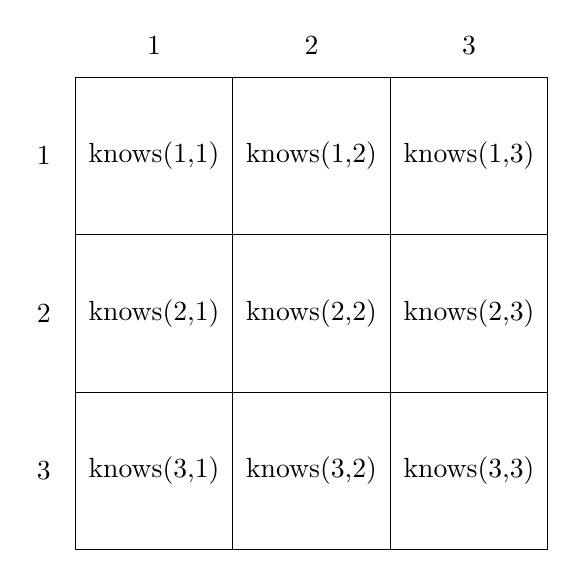
\begin{tikzpicture}[scale=2]
% Draw the numbers outside the matrix
\foreach \i in {1,...,3}
{
\draw (0.3,-\i) node{\i};
\draw (\i,-0.3) node{\i};
}
% Draw the matrix
\foreach \x in {1,...,3}
\foreach \y in {1,...,3}
{
\draw (\x,-\y) +(-.5,-.5) rectangle ++(.5,.5);
\draw (\x,-\y) node (n\y\x) {knows(\y,\x)}; %reverse the x and y to give the expected behaviour
}
\end{tikzpicture}
\end{center}
Think about what this matrix would look like given the conditions of the party in the question.
I draw a $9 \times 9$ matrix here, but you can quickly draw a smaller one to get the gist of it.
The important thing to realise is that David Beckham’s row will be empty, and his columns will be filled with ones (except for the diagonal element).
\begin{center}
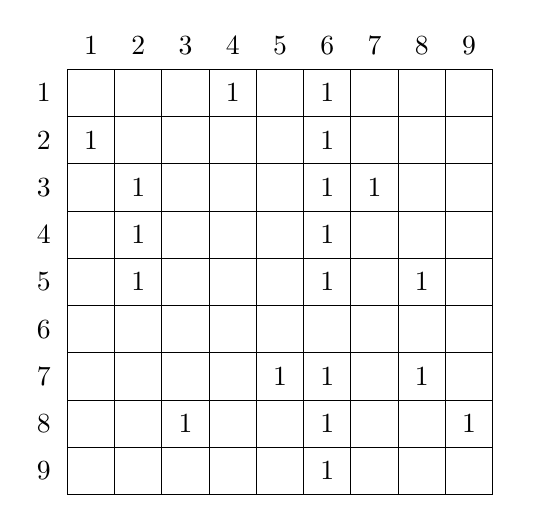
\begin{tikzpicture}[scale=0.6]
% Draw the numbers outside the matrix
\foreach \i in {1,...,9}
{
\draw (0,-\i) node{\i};
\draw (\i,0) node{\i};
}
% Draw the matrix
\foreach \x in {1,...,9}
{
  % Make nodes on the outside of the matrix on the right side
  % Label them with o1, o2, etc.
  \draw (10,-\x) node (o\x) {};
  \foreach \y in {1,...,9}
  {
    \draw (\x,-\y) +(-.5,-.5) rectangle ++(.5,.5);
    % Make the node a circle for space reasons, but don't draw it
    \draw (\x,-\y) node[circle, inner sep=2mm] (n\y\x) {}; %reverse the x and y to give the expected behaviour
  }
}
% Draw some ones
% David Beckham is person 6
% %Everyong knows someone, except Beckham
\draw (n14) node{1};
\draw (n21) node{1};
\draw (n32) node{1} (n37) node{1};
\draw (n42) node{1};
\draw (n52) node{1} (n58) node{1};
% Beckham's row
\draw (n78) node{1} (n75) node{1};
\draw (n83) node{1} (n89) node{1};

%Everyone knows David Beckham
\draw (n16) node{1};
\draw (n26) node{1};
\draw (n36) node{1};
\draw (n46) node{1};
\draw (n56) node{1};
\draw (n76) node{1};
\draw (n86) node{1};
\draw (n96) node{1};
\end{tikzpicture}
\end{center}
You can use the function to fill in values until you find David Beckham,
but filling the whole matrix is expensive. For $n$ people, you would need $n^2$ evaluations of the function.
You need to find a smarter way to find Beckham's row.

Start with person 1 and find the first non-zero entry for their row.
You have now learned two things:
\begin{enumerate}
  \item Person 1 is not David Beckham, because Beckham doesn't know anyone at the party
  \item All the people who person 1 doesn't know can be disregarded: they are not Beckham (Everyone at the party knows David Beckham, so if person 1 doesn't know you, you \emph{can't} be David Beckham)
\end{enumerate}
The second point is the crux.
If you don't identify it immediately, talk through the problem and hopefully the interviewer will nudge you in the right direction.
You will use this knowledge to rapidly discount whole blocks of people as ``not Beckham''.
Start at person 1 and check their row.
When you find a one, we jump to that person (who might be David Beckham).
Every zero you find discounts its corresponding person as not being Beckham; conversely, when you find a one, you know the current person is also not Beckham.
If you get to the end of any row, that row represents David Beckham.
This method only requires $n$ evaluations of the function since we just need to traverse all the columns, as seen in the diagram below:

\begin{center}
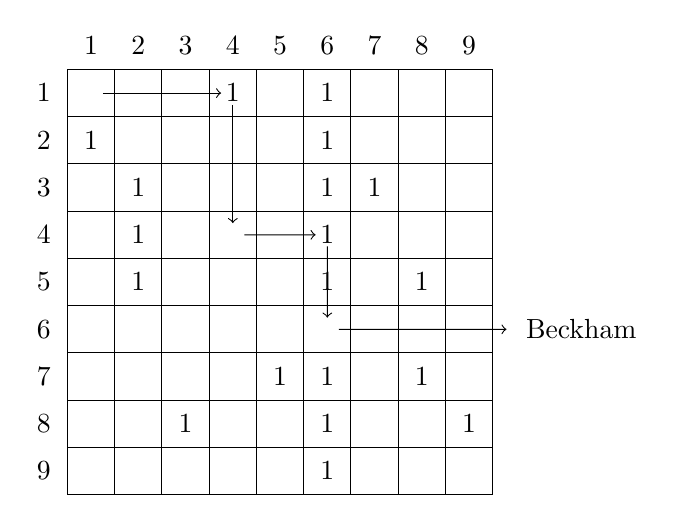
\begin{tikzpicture}[scale=0.6]
% Draw the numbers outside the matrix
\foreach \i in {1,...,9}
{
\draw (0,-\i) node{\i};
\draw (\i,0) node{\i};
}
% Draw the matrix
\foreach \x in {1,...,9}
{
  % Make nodes on the outside of the matrix on the right side
  % Label them with o1, o2, etc.
  \draw (10,-\x) node (o\x) {};
  \foreach \y in {1,...,9}
  {
    \draw (\x,-\y) +(-.5,-.5) rectangle ++(.5,.5);
    % Make the node a circle for space reasons, but don't draw it
    \draw (\x,-\y) node[circle, inner sep=1mm] (n\y\x) {}; %reverse the x and y to give the expected behaviour
  }
}
% Draw some ones
% David Beckham is person 6
% %Everyong knows someone, except Beckham
\draw (n14) node{1};
\draw (n21) node{1};
\draw (n32) node{1} (n37) node{1};
\draw (n42) node{1};
\draw (n52) node{1} (n58) node{1};
% Beckham's row
\draw (n78) node{1} (n75) node{1};
\draw (n83) node{1} (n89) node{1};

%Everyone knows David Beckham
\draw (n16) node{1};
\draw (n26) node{1};
\draw (n36) node{1};
\draw (n46) node{1};
\draw (n56) node{1};
\draw (n76) node{1};
\draw (n86) node{1};
\draw (n96) node{1};

\draw[->] (n11) to (n14);
\draw[->] (n14) to (n44);
\draw[->] (n44) to (n46);
\draw[->] (n46) to (n66);
\draw[->] (n66) to (o6) node[anchor=west]{Beckham};

\end{tikzpicture}
\end{center}

If Victoria Beckham is also at a party with nine people, the matrix might look like the following example, where David and Victoria are individuals 4 and 6:
\begin{center}
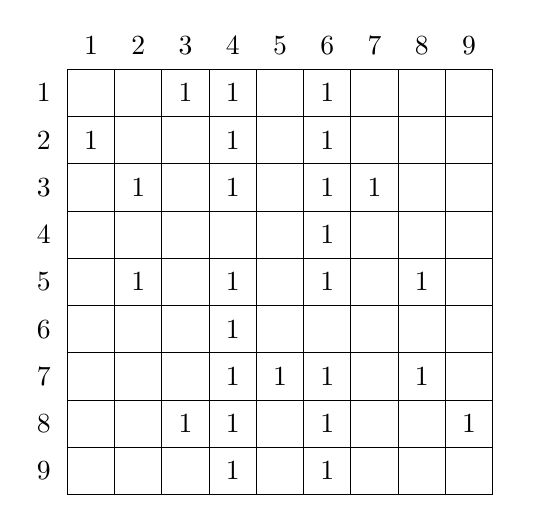
\begin{tikzpicture}[scale=0.6]
% Draw the numbers outside the matrix
\foreach \i in {1,...,9}
{
\draw (0,-\i) node{\i};
\draw (\i,0) node{\i};
}
% Draw the matrix
\foreach \x in {1,...,9}
{
  % Make nodes on the outside of the matrix on the right side
  % Label them with o1, o2, etc.
  \draw (10,-\x) node (o\x) {};
  \foreach \y in {1,...,9}
  {
    \draw (\x,-\y) +(-.5,-.5) rectangle ++(.5,.5);
    % Make the node a circle for space reasons, but don't draw it
    \draw (\x,-\y) node[circle, inner sep=2mm] (n\y\x) {}; %reverse the x and y to give the expected behaviour
  }
}
% Draw some ones
% David Beckham is person 6
% %Everyong knows someone, except Beckham
\draw (n13) node{1};
\draw (n21) node{1};
\draw (n32) node{1} (n37) node{1};
 %Victoria's row
\draw (n52) node{1} (n58) node{1};
 % Beckham's row
\draw (n78) node{1} (n75) node{1};
\draw (n83) node{1} (n89) node{1};


%Everyone knows David Beckham and Victoria
\draw (n14) node{1} (n16) node{1};
\draw (n24) node{1} (n26) node{1};
\draw (n34) node{1} (n36) node{1};
\draw               (n46) node{1};
\draw (n54) node{1} (n56) node{1};
\draw (n64) node{1}              ;
\draw (n74) node{1} (n76) node{1};
\draw (n84) node{1} (n86) node{1};
\draw (n94) node{1} (n96) node{1};

\end{tikzpicture}
\end{center}
The same logic as before applies.
Start at the first person, and ask whether they know person $2, 3, 4, \ldots, n$.
Each individual they don't know can be discounted as \emph{neither} Victoria \emph{nor} David.
The last two people we visit using this method are David and Victoria Beckham.
(We cannot identify which is which, but we weren't asked to.)
Below, the final diagram shows how to traverse the matrix:
\begin{center}
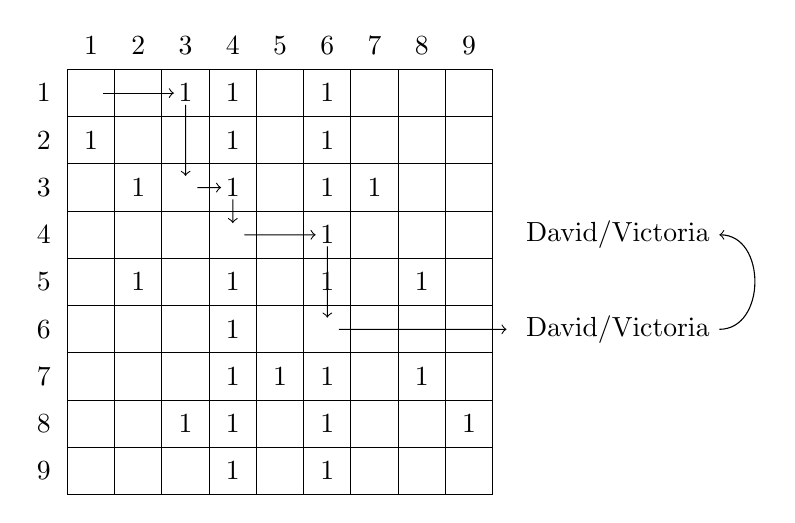
\begin{tikzpicture}[scale=0.6]
% Draw the numbers outside the matrix
\foreach \i in {1,...,9}
{
\draw (0,-\i) node{\i};
\draw (\i,0) node{\i};
}
% Draw the matrix
\foreach \x in {1,...,9}
{
  % Make nodes on the outside of the matrix on the right side
  % Label them with o1, o2, etc.
  \draw (10,-\x) node (o\x) {};
  \foreach \y in {1,...,9}
  {
    \draw (\x,-\y) +(-.5,-.5) rectangle ++(.5,.5);
    % Make the node a circle for space reasons, but don't draw it
    \draw (\x,-\y) node[circle, inner sep=1mm] (n\y\x) {}; %reverse the x and y to give the expected behaviour
  }
}
% Draw some ones
% David Beckham is person 6
% %Everyong knows someone, except Beckham
\draw (n13) node{1};
\draw (n21) node{1};
\draw (n32) node{1} (n37) node{1};
 %Victoria's row
\draw (n52) node{1} (n58) node{1};
 % Beckham's row
\draw (n78) node{1} (n75) node{1};
\draw (n83) node{1} (n89) node{1};


%Everyone knows David Beckham and Victoria
\draw (n14) node{1} (n16) node{1};
\draw (n24) node{1} (n26) node{1};
\draw (n34) node{1} (n36) node{1};
\draw               (n46) node{1};
\draw (n54) node{1} (n56) node{1};
\draw (n64) node{1}              ;
\draw (n74) node{1} (n76) node{1};
\draw (n84) node{1} (n86) node{1};
\draw (n94) node{1} (n96) node{1};

\draw[->] (n11) to (n13);
\draw[->] (n13) to (n33);
\draw[->] (n33) to (n34);
\draw[->] (n34) to (n44);
\draw[->] (n44) to (n46) ;
\draw[->] (n46) to (n66);
\draw[->] (n66) to (o6);
\node (exita) at (o6) [anchor=west] {David/Victoria};
\node (exitb) at (o4) [anchor=west] {David/Victoria};
\draw[->] (exita.east) .. controls ++(1,0) and ++(1,0) .. (exitb.east);

\end{tikzpicture}
\end{center}
This question tests your knowledge of applied graph or network theory, and it has more to do with computer algorithms than mathematics.
\index{graph theory}
While these kinds of questions aren't that prevalent, they are increasingly common at some hedge funds and high-frequency trading firms who emphasise algorithms and programming skills.
If you are required to do a pre-interview coding test, chances are you will see a graph theory problem.
They used to be popular in Google interviews back when they still asked brainteasers.
Google has since stopped doing it after discovering that brainteaser performance was a bad predictor of actual job performance.\footnote{See, for instance, this newspaper article by \citet{GoogleBrainteasers}.}

\end{answer}

\begin{answer}{arrayofintegersfindduplicate}
 Without sorting, you have to keep track of the numbers you have seen.
 You could mention using a hashtable, or some other container with key-value pairs.
 The Python \verb+dict+ is an example.
 That way you can quickly check whether each number is already in the dictionary, and stop looking if you find that it is.
 If the number isn't in the dictionary, add it.
 The Python \verb+defaultdict+ is even better, as it handles the key error when the key is not yet in the dictionary.
 You can also  add the values into a list in such a way that the list remains sorted.
 For each integer, you then do a binary search on the list to see whether the integer is already there.
 This is the basic idea of a binary tree.
 Think of a few ways to do this using various containers in your favourite language, and think of their respective benefits.
 This question has many solutions, and there are no wrong answers.

 Answering the question with sorting is much easier.
 Sort the numbers, go through them one by one, and ask ``Is the next value equal to the current value?''
 As soon as the answer is ``yes'', stop the search.
 The question about your favourite sorting algorithm is a loaded one.
 The interviewer is likely to ask you to explain how it works, about its complexity, and to write it in actual or pseudocode.
 Therefore, ensure you do have a favourite sorting algorithm and make sure you know its details.
 Also, ensure your favourite isn't Bubblesort---it is inefficient and acts only as an example to get new programmers thinking about algorithms.
 It is also overused by people doing interviews.
Your favourite sorting algorithm should be Mergesort, for the following reasons:
\index{mergesort}
 \begin{enumerate}
   \item Efficiency---it has $O(n \log n)$ complexity, which is on par with the best sorting algorithms used in production
   \item Practicality---it is actually used in production, though usually as part of more efficient algorithms such as Timsort
   \item Parallelisation---its divide-and-conquer strategy has obvious benefits when used with computing clusters and GPU programming
   \item Simplicity---the main workings only require six lines of code. See the example below.
 \end{enumerate}
The basic idea of Mergesort is splitting the list into two parts, sorting each part, and re-combining them into single, sorted list.
Since the second step requires sorting, you can do it recursively.
The workings are given in the below pseudocode, where the assumption is that a function exists called
MergeTwoSortedVectors()
which receives two sorted vectors as arguments and combines them into one sorted vector:
\begin{algorithmic}[1]
  \Statex
  \Function{MergeSort}{$\vec{x}$}
  \State
        $n$ = length($\vec{x}$)
    \If{n is 1}
      \State
      \Return $\vec{x}$
      \Comment{ Recursion base case}
     \EndIf
  \State
  $m$ = round($\nicefrac{n}{2}$) \Comment Vector middle index
  \State
  firsthalf = $\{x_1, x_2, \ldots ,x_m\}$
  \State
  secondhalf = $\{x_{m+1}, x_{m+2}, \ldots, x_n \}$
  \State
  firsthalf\_sorted = MergeSort(firsthalf)
  \Comment Recursive call
  \State
  secondhalf\_sorted = MergeSort(secondhalf)
      \State \Return{ MergeTwoSortedVectors(firsthalf\_sorted, secondhalf\_sorted) }
  \EndFunction
\end{algorithmic}
The code is simple since most of the tricky workings are hidden in the MergeTwoSortedVectors() function.

The Python implementation of Mergesort below is even easier to read than the pseudocode:
\begin{minted}[samepage=true]{python}
def mergesort(unsortedlist):
    if (len(unsortedlist)==1):
        return unsortedlist

    mid = len(unsortedlist)/2
    firsthalf = unsortedlist[0:mid]
    secondhalf = unsortedlist[mid:]
    return merge(mergesort(firsthalf), mergesort(secondhalf))
\end{minted}
One way to have Python do the merge function is:
\begin{minted}[samepage=true]{python}
# These two lists will already be sorted from small to large
def merge(list1, list2):
    sortedlist = []
    while ((len(list1)>0) or (len(list2) > 0)):
        if (len(list1)==0):
            return list2 + list(reversed(sortedlist))
        elif (len(list2)==0):
            return list1 + list(reversed(sortedlist))
        else:
            if (list1[-1] >= list2[-1]):
                sortedlist.append(list1.pop())
            else:
                sortedlist.append(list2.pop())

\end{minted}
\end{answer}

\begin{answer}{criminalsinfield}
  The solution to this question requires many assumptions on the rationality of the criminals which probably don't hold in practice.
  You should also ask some further questions to establish that you are allowed to address the criminals before they make a run for it, which probably means you have a very loud voice or a megaphone.
  Good interviewers will tell you this as part of the question, while others might want you to prod.

  Start with $n=1$.
  \index{tricks!start with simplest case}
  Were there a single murderer, you would shoot him if he tried to escape.
  Because he would know the probability of survival is zero, he wouldn't try.
  Were there only two murderers in the field, each would have a probability of surviving of 0.5, and thus would attempt to escape.
  But, if you told one of the two that you would definitely shoot \emph{him} if the two of them attempted to escape, he wouldn't make an attempt, bringing you back to the situation with a single murderer.
  You can generalise this outcome to three or more murderers, but for any given group you need to identify one murderer as the so-called ``sacrificial escapee'', and make him aware of it.
  The easiest way is to number them from $1$ to $n$, and tell them that, for any group that attempts an escape, the member with the largest number will be shot.
  By induction, no group will attempt an escape.
  If you don't have time to number them, the go-to solution is to tell the murderers that, in the event of an attempted escape, the tallest member of the group will be shot.

  Though this is an illogical question, try not to get frustrated and point this out to the interviewer.
  It is asked in the same spirit as questions such as ``how many ping pong balls can fit into an Airbus A380,'' or ``how many ties are sold in London in a year.''
  The interviewer wants to see your thought process.
  Through all of my interviews I only got a question like this once and while I think they are rare in quantitative interviews, I believe they are more prevalent in investment banking interviews in general.
  I would suggest you look up two or three of these, and study the format of the solutions.
\end{answer}



\clearpage
\subsection{Phone interview, 45 minutes}
\begin{question}{regressiontheory2}
\index{questions!regression theory}
What are the significance tests used for the parameters estimated in a logistic regression?
How are they different than those used for a linear regression?
\end{question}


\begin{question}{twopiecesofwood}
\index{questions!measure pieces of wood}
You have two pieces of wood of length $a$ and $b$, where $a<b$, and a measuring apparatus with a variance of $\sigma^2$, due to measurement error.
It costs \pounds 1 per use.
You only have \pounds2.
What is the best strategy to measure $a$ and $b$ with minimal variance?
\end{question}



\begin{question}{bagnsockstwored}
\index{questions!bag of socks}
A bag contains $N$ socks, some of which are black, and some of which are red.
If two random socks are picked, the probability that they are both red is $\nicefrac{1}{2}$.
What is the smallest possible value of $N$ for which this is possible?
\end{question}

\clearpage
\begin{answer}{regressiontheory2}
For this question, which is like question \ref{q:regressiontheory1}, familiarise yourself with the material in section \ref{sec:regressiontheory}.
\end{answer}

\begin{answer}{twopiecesofwood}
This is a great question.
Start with the naive approach.
If we measure $a$ and $b$ on their own, we get
\begin{align*}
\E(a)   &= a \\
\Var(a) &= \sigma^2 \\
\E(b)   &= b \\
\Var(b) &= \sigma^2
\end{align*}
We've measured each one with an error of $\sigma^2$.
We can do better.
We can measure the sum of the two sticks, $s = a+b$, and the difference between the two $d = a-b$.
\begin{center}

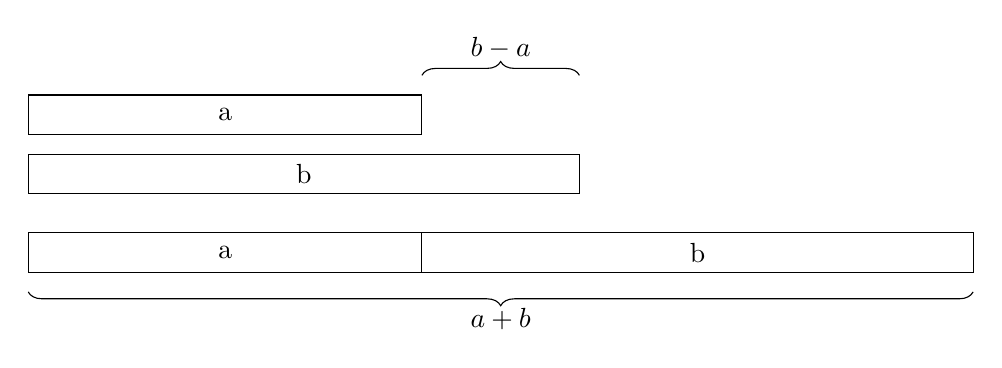
\begin{tikzpicture}
\draw (0,0.75) rectangle ++(5,0.5)node[midway]{a};
\draw (0,0)    rectangle ++(7,0.5) node[midway]{b};
\draw[decorate, decoration={brace, amplitude=5pt}]
      (5,1.5) -- (7,1.5) node (A) [midway, yshift=10pt]{$b-a$};

\draw (0,-1) rectangle ++(5,0.5)node[midway]{a};
\draw (5,-1)    rectangle ++(7,0.5) node[midway]{b};
\draw[decorate, decoration={brace, mirror, amplitude=5pt}]
      (0,-1.25) -- (12,-1.25) node (A) [midway, yshift=-10pt]{$a+b$};
\end{tikzpicture}

\end{center}
Let us solve for $a$ and $b$ in terms of $s$ and $d$, and see what the mean and variance of our estimates are.
\begin{align*}
a   &= \frac{s - d}{2} \\
\E(a)  &= \E\left(\frac{s - d}{2}\right)
        =  a \\
\Var(a) &= \Var\left(\frac{s - d}{2} \right) \\
        &= \frac{1}{4}(\Var(s) + \Var(d)) \\
        &= \frac{1}{2}\sigma^2 \\
        & \quad \text{Likewise, for } b \\
b   &= \frac{s + d}{2} \\
\E(b)  &= \E\left(\frac{s + d}{2}\right)
        =  b \\
\Var(b) &= \Var\left(\frac{s + d}{2} \right) \\
        &= \frac{1}{2}\sigma^2
\end{align*}
What happened here? As if by magic, we were able to reduce our variance by half.
The trick is that we used our tools to measure $a$ and $b$ twice.
Each additional measurement will reduce the variance of our estimator.
\end{answer}

\begin{answer}{bagnsockstwored}
Let $R_i$ indicate the event where the $i$th sock is red.
Let $r$ be the number of red socks in a bag of $N$ socks.
You need
\begin{align*}
  P(R_1,R_2)     &= \frac{1}{2} \\
  P(R_1)(R_2|R_1) &= \frac{1}{2} \\
  \frac{r}{N} \times
  \frac{r-1}{N-1}
   &=
  \frac{1}{2}
  \text{.}
\end{align*}
Use trial and error.
\index{tricks!start with simplest case}
If $N=2$ both socks will be red with certainty, so this cannot work.
When $N=3$ you have
\[
  \frac{r}{3} \times
  \frac{r-1}{2}
   =
  \frac{r(r-1)}{6}
   =
  \frac{1}{2}
\]
and there aren't any integer values of $r$ that would make this hold.
For $N=4$ you have
\[
  \frac{r}{4} \times
  \frac{r-1}{3}
   =
  \frac{r(r-1)}{12}
   =
  \frac{1}{2}
\]
and this works for $r=3$.
Therefore, the smallest possible value of $N$ is four.
\end{answer}



\clearpage
\subsection{Onsite, 5 interviews, 3 hours}
\begin{question}{regressiontheory3}
\index{questions!regression theory}
What are the assumptions required for a linear regression?
What is multicollinearity, and what are its implications?
How would you measure goodness of fit?
\end{question}


\begin{question}{nameafewnonlinearmodels}
\index{questions!non-linear models}
What are some non-linear models?
\end{question}


\begin{questionwithnoanswer}
\index{questions!SQL}
Write some SQL queries.
Consider a table with the following headings:
\begin{center}
\begin{tabular}{|c|c|c|}
\hline
   Employee name & Department & Salary \\
\hline
\end{tabular}
\end{center}
\end{questionwithnoanswer}

\begin{subquestion}{sqladdaveragesalary}
Add a column to show the average department salary for each employee.
\end{subquestion}


\begin{subquestion}{sqlhighestsalary}
Write a query to return the second highest salary.
\end{subquestion}



\begin{question}{sqlfindcustomerswithchanges}
You are given the following table:
\begin{center}
\begin{tabular}{|c|c|c|c|}
\hline
     Customer ID    &   Name     &  datestart     & dateend     \\
\hline
     A              &   Jon      &  1991-05-06    & 1992-05-06  \\
     A              &   Jonathan &  1992-05-06    & 1998-10-02  \\
     B              &   Chris    &  1983-01-01    & 1997-12-16  \\
     C              &   Sean     &  1991-05-06    & 2000-05-12  \\
\hline
\end{tabular}
\end{center}
Write a query to return all the customers who have made changes to their details.
\end{question}

\clearpage
\begin{answer}{regressiontheory3}
This is the same question as \ref{q:regressiontheory1} and \ref{q:regressiontheory2}.
These questions are frequently asked for quantitative roles, so make sure you study section \ref{sec:regressiontheory}.
\end{answer}

\begin{answer}{nameafewnonlinearmodels}
Some examples of non-linear models are:
\begin{itemize}
  \item Survival models, which usually study a non-linear hazard rate $h(t)$
  \item Generalised Linear Model (GLM), which can have non-linear link functions
  (the logistic regression uses the logit link function, and the Gamma GLM uses the log link function)
  \item Gaussian processes (and other non-parametric regressions)
  \item Neural networks, which are an approximation of Gaussian processes, as shown by \citet[chap.~15.4]{murphy2012machine} using the proof that was first pointed out by  \citet{neal1996bayesian}: as the number of hidden layers in a neural net goes to infinity, it becomes a Gaussian process
\end{itemize}
In fact, a broad class of non-linear models can be presented in the following way:
\begin{align*}
  y \sim
  \operatorname{MultivariateNormal}( g(X,\theta), \Sigma )
\end{align*}
where $g(X,\theta)$ is some non-linear function of the parameters and the inputs.
You can make this more general by replacing the multivariate normal distribution,
\begin{align*}
  y \sim Dist( g(X,\theta) )
\end{align*}
where $y$ is assumed to follow some distribution and $g(X, \theta)$ is some function that links the inputs to the parameters of the distribution.
See \citet{murphy2012machine} for an exhaustive treatment of this idea.

\end{answer}

\begin{subanswer}{sqladdaveragesalary}

\begin{minted}{sql}
SELECT
    Employee_name,
    a.Department,
    Salary,
    avg_dept_sal
from salaries as a
INNER JOIN
(   SELECT
        Department,
        avg(Salary) as avg_dept_sal
    from salaries
    GROUP BY Department
) as b
where a.Department = b.Department
\end{minted}
I include code to create the table and execute this query in appendix \ref{ap:sqlite}.
\end{subanswer}

\begin{subanswer}{sqlhighestsalary}
There are many ways to do this, involving merges, sorts and joins.
I find the easiest and clearest way is to use \verb+LIMIT+ and \verb+OFFSET+, which exist in all SQL implementations.
The logic is to sort descending by salary, then offset the rows by one, and return only one entry.
The result will be the second highest entry.
You can easily change the offset to return the $n$th highest salary:
\begin{minted}{sql}
SELECT
    Employee_name,
    Department,
    Salary
FROM salaries
ORDER BY Salary DESC
LIMIT 1
OFFSET 1
\end{minted}
Appendix \ref{ap:sqlite} contains code to load the table and test this query.
\end{subanswer}

\begin{answer}{sqlfindcustomerswithchanges}
We have to look at the table and make an assumption on which columns will give us this information.
It seems that we need to find the entries in the \verb+Customer ID+ column that appear multiple times.
When a customer changes their details, they keep the same ID.
When we want to test conditions on calculated columns, we need to use
\verb+HAVING+
instead of
\verb+WHERE+.
\begin{minted}{sql}
SELECT CustomerID
FROM customers
GROUP BY CustomerID
HAVING count(CustomerID) > 1
\end{minted}
As with the previous question, appendix \ref{ap:sqlite} contains code to load the table and test this query.
As is evidence from the questions so far, SQL questions aren't that common.
During my interview, the interviewer asked me whether I was familiar with SQL before asking these questions (I listed it on my CV).
If it wasn't on my CV and had I answered ``no'', they probably would have asked me data-cleaning questions in other languages.

Practising SQL is tedious due to the amount of work required to get it working on your system.
Some installations---like OracleDB or Microsoft SQL server---are prohibitively expensive for someone who just wants to practise.
Postgresql and MySQL are free and open source, but they require multiple libraries to be installed and access management to be configured (even if you just want to run queries locally).
It might be worth the effort, however, to get an understanding of the architecture.
The path of least resistance is certainly sqlite, used with Python.
Most Python installations come with sqlite as standard, so it doesn't require any other libraries.
I suggest using the code included in \ref{ap:sqlite} along with a dataset you are familiar with to do some cleaning and munging using queries (as opposed to using R or Pandas data frames).
Especially if you list SQL on your CV, but haven't used it recently.
Thereafter, if you want more rigour, try MySQL.
\end{answer}



\clearpage
\subsection{Face-to-face, 2 hours}
\begin{question}{regressiontheory4}
\index{questions!regression theory}
What assumptions are needed for a linear regression?
Are they the same for a logistic regression?
How would you test the significance of the parameters for a linear regression?
Would you use the same test in the case of a logistic regression?
\end{question}


\begin{questionwithnoanswer}
Answer the following questions about R.
\end{questionwithnoanswer}

\begin{subquestion}{rdatastructures}
\index{questions!R!data structures}
What are some data structures used in R?
\end{subquestion}



\begin{subquestion}{rmergetwodataframes}
\index{questions!R!merge data frames}
Describe the syntax you would use to merge two data frames.
\end{subquestion}



\begin{subquestion}{rapplyvsforloops}
\index{questions!R!L@\verb+lapply+ vs for loop}
What is the difference between \verb+lapply()+ and for-loops?
Which do you prefer?
\end{subquestion}


\begin{question}{grownup}
Here is a specific problem the team faced last year.
What model will you build to solve it, and why?
\end{question}

 \clearpage
\begin{answer}{regressiontheory4}
This question is similar to questions
\ref{q:regressiontheory1},
\ref{q:regressiontheory2}, and
\ref{q:regressiontheory3}, and is answered in section \ref{sec:regressiontheory}.
\end{answer}

\begin{answer}{rdatastructures}
\begin{itemize}
  \item Lists, which are like Python dictionaries, but don't necessarily require its contents to be named.
  They can contain multiple data types, and can contain other containers like vectors, matrices, or further nested lists.
  They can also contain functions.
  \begin{minted}{r}
mylist <- list(key1=c(1,2,3),
               key2="hello world",
               list(a=1, b="2"))
  \end{minted}
  \item Vectors, which don't have a dimension until you coerce it into an array or matrix.
  That means they aren't considered to be row or column vectors.
  They can only contain data of one type.
  They cannot contain other data structures like lists or vectors.
  \begin{minted}{r}
myvec1 <- c(1,2,3)
myvec2 <- 1:10
myvec3 <- c("one","two", "three")
  \end{minted}
  \item
  Factors, which are a special case of vectors in R that contain categorical data.
  They can be ordered, for instance \verb+c("high", "medium", "low")+.
  These form an important part of the R language since all the estimation and fitting libraries contain procedures to deal with them, like assigning dummy variables automatically.
  They also reduce storage, since long strings are stored as numbers.
  \item Matrices and arrays.
  These are multidimensional vectors.
  While matrices are two-dimensional arrays, it is important to have them as a distinct type to allow for matrix arithmetic.
  \begin{minted}{r}
mymatrix <- matrix(1:100, 10, 10)
myarray <-  array(1:1000, dim=c(10,10,10))
  \end{minted}
  \item Data frames. This is R's native ``table data'' format.
  Each column is a vector with one data type, and each row represents an observation in the dataset.
  \item Data tables. This is a relatively new library for R, written by \citet{datatables}.
  The library has a powerful C++ back end, and allow users to handle big datasets in R.
  Most of the operations occur in memory, as opposed to data frames which have a tendency to create copies.
  These can be thought of as R's answer to the \verb+pandas+ library in Python.
  They have a wholly different syntax than that of data frames.
\end{itemize}
\end{answer}

\clearpage
\begin{answer}{rmergetwodataframes}
\begin{minted}{r}
df3 <- merge(df1, df2, by="colname")

df3 <- merge(df1, df2,
             by.x="x_colname",
             by.y="y_colname",
             all.x=TRUE,
             all.y=TRUE)
\end{minted}
The second statement will perform a full outer join.
Merging data frames are a very important part of data cleaning.
Make sure you can do it in all the languages you use, as well as SQL.
\end{answer}

\begin{answer}{rapplyvsforloops}
 To the user, the main difference is in the syntax.
 To the machine, there are many differences in the implementation, especially concerning memory allocation and optimisations.
 The question specifies \verb+lapply+, which applies a function over a list and returns a list.
 Here is some code that will take every item in a list of integers, and apply a function to multiply it by two.
 Also given is the for-loop for the same action.

\begin{minted}{r}
mult2 <- function(x) return(x*2)

listofintegers <- list(1,2,3)
ans1 <- lapply( listofintegers , mult2)

ans2 <- list() # initialize empty list
for (i in 1:length(listofintegers)){
  ans2[[i]] <- mult2(listofintegers[[i]])
}
\end{minted}
There might be better ways to write the for-loop, but this suffices to highlight the difference.
As for the question about preference: you should prefer \verb+lapply+ due to all the optimisation that comes with vectorisation.
The developers of the R created these functions for a reason.
It is also easy to parallelise code written with \verb+lapply+.
The biggest caveat of these functions, however, is readability.
\end{answer}

\begin{answer}{grownup}
This is an opportunity to align your skills and experience to the team's needs.
Make sure your answers are in line with your area of expertise---even if you don't consider it wholly relevant.
Display your specialist knowledge and experience, and how you use it to solve an unfamiliar problem.
Your job as a quant will involve solving problems using mathematics.
You need to be able to do this often, and do it quickly.

Do not fall victim to hype.
For instance, don't use neural nets just because they are in fashion.
Stick with what you know.
If you want to show that you are well-read on the Zeitgeist of \emph{analytics} hype, mention how your answer is different from neural nets---or whatever is in fashion---and outline the benefits and caveats of both approaches.
If you are asked to discuss a particular topic you don't know much about, be honest about your limitations.
Often the interviewer isn't trying to catch you out, they are merely curious about the extent of your knowledge and your willingness to learn.

\end{answer}


\clearpage
\subsection{Video interview, 1 hour}
\begin{question}{simplerandomwalkhittingprobability}
\index{questions!simple random walk hitting probability}
You have a simple random walk,
\[
  X_t = \sum_{i=1}^{t}{Z_i}
\]
where
\begin{align*}
 P(Z_i =  1) &= 0.5 \\
 P(Z_i = -1) &= 0.5
 \text{.}
\end{align*}
If the process is currently at $k$, meaning $X_0=k$, what is the probability that it would hit $l$ before hitting $0$,
where $k < l$?
\end{question}

\clearpage
\begin{answer}{simplerandomwalkhittingprobability}
This deceptively simple-looking question is difficult and requires specialist theory to solve.
During an interview, never say you do not know.
Even if you are certain you do not know the theory required, use the first trick in appendix \ref{ap:tricks} and start with the trivial case.
\index{Tricks!Start with simplest case}
Here, it means we start the process at $k=1$ and let $l=2$.
Then the process can go either way with probability $\frac{1}{2}$.
Next, consider $l=3$ where the process can be at $k=1$ or $k=2$.
Let $A_k$ be the event that the process currently at $k$ reaches three before it reaches zero.
The process has two places it can be and they depend on each other in the following manner,
\begin{align*}
P(A_2) &= (0.5)(1) + (0.5)P(A_1)  \\
P(A_1) &= (0.5)(0) + (0.5)P(A_2)
\text{.}
\end{align*}
Write everything in terms of $P(A_1)$ to solve it,
\begin{align*}
P(A_1) &= 0 + (0.5) \Big((0.5)(1) + (0.5) P(A_1)\Big) \\
P(A_1) &= \frac{1}{4} + \frac{1}{4}P(A_1) \\
P(A_1) \left(\frac{3}{4}\right)&= \frac{1}{4} \\
P(A_1) &= \frac{1}{3}
\text{.}
\end{align*}
Then we can also solve for $P(A_2)$,
\begin{align*}
P(A_2) &= \frac{1}{2} + \frac{1}{2} P(A_1)  \\
       &= \frac{1}{2} + \frac{1}{2}\left(\frac{1}{3}\right) \\
       &= \frac{2}{3}
\text{.}
\end{align*}
This is how I started attempting the question and the interviewer seemed content before I reached a clear answer, then moved on to questions about my current role.

For the sake of completeness, let us solve one more case where $l=4$ to see whether a pattern emerges.
Let $A_k$ be the event that the process currently at $k$ reaches four before it reaches zero.
The process now has three places it can be,
\begin{align*}
P(A_3) &= (0.5)(1) + (0.5)P(A_2)  \\
P(A_2) &= (0.5)P(A_3) + (0.5)P(A_1) \\
P(A_1) &= (0.5)(0) + (0.5)P(A_2)
\text{.}
\end{align*}
Let's write everything in terms of $P(A_3)$,
\begin{align*}
P(A_2) &= (0.5)P(A_3) + (0.5)\Big(0 + (0.5) P(A_2) \Big)  \\
P(A_2) &= (0.5) P(A_3)  + (0.25) P(A_2)  \\
P(A_2) &= \frac{2}{3} P(A_3)
\end{align*}
\begin{align*}
P(A_3) &= (0.5)(1) + (0.5) P(A_2)   \\
       &= \frac{1}{2} + \frac{1}{2}\left(\frac{2}{3}P(A_3)\right)  \\
            P(A_3) &= \frac{3}{4}
\text{.}
\end{align*}
Use this result to get $P(A_2)$,
\begin{align*}
P(A_2) &= \frac{2}{3} P(A_3)  \\
       &= \frac{2}{3}\left(\frac{3}{4}\right) \\
       &= \frac{1}{2}
\end{align*}
and finally $P(A_1)$
\begin{align*}
P(A_1) &= \frac{1}{2} P(A_2)        \\
       &= \frac{1}{2}\left( \frac{1}{2} \right) \\
       &= \frac{1}{4}
\text{.}
\end{align*}
It is clear that using this method to find a general solution for $k$ and $l$ would be tedious.
For the case where $l=4$ we ended up with the formula
\begin{align*}
P(A_k) &= \frac{k}{4}
\text{.}
\end{align*}
It is alluring to suggest general answer should be
$P(A_k) = \nicefrac{k}{l}$.
If we write down the equations for the general case we have
\begin{align*}
P(A_1) &= (0.5)(0)      + (0.5) P(A_2)  \\
P(A_2) &= (0.5) P(A_1)  + (0.5) P(A_3)  \\
P(A_3) &= (0.5) P(A_2)  + (0.5) P(A_4)  \\
 & \vdots \\
P(A_{l-2}) &= (0.5) P(A_{l-3})  + (0.5) P(A_{l-1})  \\
P(A_{l-1}) &= (0.5) P(A_{l-2})  + (0.5)(1)
\end{align*}
which we can rewrite as
\begin{align*}
0 &= (0.5)(0) - P(A_1)   + (0.5)(P(A_2)) \\
0 &= (0.5) P(A_1)  - P(A_2)  + (0.5) P(A_3)  \\
0 &= (0.5) P(A_2)  - P(A_3)  + (0.5) P(A_4)  \\
  & \vdots \\
0 &= (0.5) P(A_{l-3})  - P(A_{l-2}) + (0.5) P(A_{l-1}) \\
0 &= (0.5) P(A_{l-2})  - P(A_{l-1}) + (0.5)(1)
\text{.}
\end{align*}
Then we have something that can also be expressed in matrix form
\begin{align*}
\vec{B}\vec{x} &= \vec{c} \\
  \begin{bmatrix}
 -1           & \frac{1}{2}  & 0            &   \ldots       & 0            & 0            \\
 \frac{1}{2}  & -1           & \frac{1}{2}  &   \ldots       & 0            & 0            \\
 0            & \frac{1}{2}  & -1           &   \ldots       & 0            & 0            \\
  \vdots      & \vdots       & \vdots       &   \ddots       & \vdots       & \vdots       \\
 0            & 0            & 0            &   \ldots       & -1           & \frac{1}{2}  \\
 0            & 0            & 0            &   \ldots       & \frac{1}{2}  & -1           \\
  \end{bmatrix}
  \begin{bmatrix}
  P(A_1) \\
  P(A_2) \\
  P(A_3) \\
  \vdots \\
  P(A_{l-2}) \\
  P(A_{l-1}) \\
  \end{bmatrix}
  &=
  \begin{bmatrix}
    0 \\ 0 \\ 0 \\ \vdots \\ 0 \\ -\frac{1}{2} \\
  \end{bmatrix}
\end{align*}
and we can use it to solve for the vector $\vec{x}$ with the probabilities
\begin{align*}
\vec{x} &= \vec{B}^{-1}\vec{c} \\
  \begin{bmatrix}
  P(A_1) \\
  P(A_2) \\
  P(A_3) \\
  \vdots \\
  P(A_{l-2}) \\
  P(A_{l-1}) \\
  \end{bmatrix}
  &=
  \begin{bmatrix}
 -1           & \frac{1}{2}  & 0            &   \ldots       & 0            & 0            \\
 \frac{1}{2}  & -1           & \frac{1}{2}  &   \ldots       & 0            & 0            \\
 0            & \frac{1}{2}  & -1           &   \ldots       & 0            & 0            \\
  \vdots      & \vdots       & \vdots       &   \ddots       & \vdots       & \vdots       \\
 0            & 0            & 0            &   \ldots       & -1           & \frac{1}{2}  \\
 0            & 0            & 0            &   \ldots       & \frac{1}{2}  & -1           \\
  \end{bmatrix}^{-1}
  \begin{bmatrix}
    0 \\ 0 \\ 0 \\ \vdots \\ 0 \\ -\frac{1}{2} \\
  \end{bmatrix}
\text{.}
\end{align*}
For the case where $l=7$, for example, we have the following,
\begin{align*}
\vec{B} &=
(-1)
\left[\begin{matrix}1 & - \frac{1}{2} & 0 & 0 & 0 & 0\\- \frac{1}{2} & 1 & - \frac{1}{2} & 0 & 0 & 0\\0 & - \frac{1}{2} & 1 & - \frac{1}{2} & 0 & 0\\0 & 0 & - \frac{1}{2} & 1 & - \frac{1}{2} & 0\\0 & 0 & 0 & - \frac{1}{2} & 1 & - \frac{1}{2}\\0 & 0 & 0 & 0 & - \frac{1}{2} & 1\end{matrix}\right]
\\
\vec{B}^{-1} &=
-
\frac{2}{7}
\left[\begin{matrix}6 & 5 & 4 & 3 & 2 & 1\\5 & 10 & 8 & 6 & 4 & 2\\4 & 8 & 12 & 9 & 6 & 3\\3 & 6 & 9 & 12 & 8 & 4\\2 & 4 & 6 & 8 & 10 & 5\\1 & 2 & 3 & 4 & 5 & 6\end{matrix}\right]
\\
\vec{B}^{-1}\vec{c}
&=
\left[\begin{matrix}\frac{1}{7} & \frac{2}{7} & \frac{3}{7} & \frac{4}{7} & \frac{5}{7} & \frac{6}{7}\end{matrix}\right]^{T}
\text{.}
\end{align*}
The matrix $B$ is nearly diagonal, and I expect there would be a way to prove the expected result using matrix theory; albeit not one that is quick enough to use during an interview.

Martingale theory provides the elegant proof.
The theory is quite heavy and it is unlikely that you will be able to solve questions using martingales without substantial practice.
In my experience interviewers are happy if you attempt the brute force solution; it allows you to show them how you would break a very difficult problem into simpler parts (and they get to see your algebra).
If you mention anything about martingales on your CV, be ready to use it to solve questions of this type as well as all the questions involving martingales in \citet{JoshiQA} and \citet{HeardOnTheStreet}.

For this question, realise that $X_t$ is a martingale.
This allows us two things.
First, we can define
the times at which the process reaches each of the bounds as stopping times,
\begin{align*}
  T_0 &= \inf\{ n \geq 0: X_n = 0\} \\
  T_l &= \inf\{ n \geq 0: X_n = l\}
  \text{.}
\end{align*}
Second, let $T$ be the first time we hit either $0$ or $l$, meaning $T = \min(T_0 , T_l)$.
Then since $X_t$ is a martingale we have
\[
E(X_T) =  E(X_0) = k
\text{.}
\]
We further have
$X_T=0$ if $T_0 < T_l$
and
$X_T=l$ if $T_0 > T_l$.
The crux is to realise that these two probabilities partition the entire probability space, such that
\begin{align*}
k = E(X_T) &=  0 P(T_0 < T_l) + l P(T_0 > T_l) \\
           &=  l P(T_0 > T_l)  \\
P(T_0 > T_l) &= \frac{k}{l}
\text{.}
\end{align*}
The probability $P(T_0 > T_l)$ is the one we are interested in and we see the result is the one we expected.
\end{answer}




\clearpage
\subsection{Phone interview, 1 hour}
\begin{question}{addnumbersgame}
\index{questions!add numbers game}
We are going to play a game using the integers between one and ten, inclusive.
You start, and say a number between one and ten.
Thereafter, I add a number between one and ten to your number and say the result.
Then it is your turn again.
You add a number between one and ten to the previous number I said.
We carry on, taking turns to add to the most recent number, and the first person to say 50 wins.
How much would you wager on this game?
\end{question}


\begin{question}{drop20cards}
\index{questions!drop 20 cards}
I have a deck of 52 cards.
I shuffle the deck, and drop 20 cards randomly into a shredder.
You then draw two cards from what remains.
What is the probability that they are both aces?
\end{question}


\clearpage
\begin{answer}{addnumbersgame}
The question about the wager is misleading, since it suggests that the outcome is random.
The crux of the question is to realise it is not.
It is easier to see this if you work backward.
If you want to win, you have to say ``$50$''.
You can only do this if the last number your opponent said was a number between $40$ and $49$.
That means, the number you have to say before that is $39$ (forcing your opponent to say a number in the range required).
Thus, saying $39$ will guarantee that you win.
You can work back further.
You can only say $39$ if the previous number you said was $28$ (forcing your opponent to say a number between $29$ to $38$, inclusive).
The number you'd have to say before that is $17$, and the first number you should say is $6$.
If you start and say ``$6$'', you will win with 100\% probability, and thus you should wager all the money at your disposal.
\end{answer}

\begin{answer}{drop20cards}
The fact that 20 cards were randomly discarded before you got to draw two has no influence on your probability of drawing aces.
This is not obvious from the way the question is framed.
Getting this question over the phone may be a hint that the answer can't be too complicated, but this is not a rule you can rely on.


One way to think about it is to pretend we are randomly dealing the deck into two groups: one group has two cards, and one group has 20.
The fact that I deal the 20 cards first doesn't affect the probability of the second group.
Another way to think about it is from the perspective of a poker game, like Texas Hold'em, where each player gets 2 cards.
You can calculate the probability of getting two aces before the cards are dealt.
Whether you are playing against two or ten other players, it doesn't affect \emph{your} probability of getting two aces on the deal.
Consider the 20 cards that are randomly being discarded in this question as the ones given to your opponents in a game.
You wouldn't think it was unfair if your opponents got their cards \emph{before} you receive yours, because it is still dealt random and thus your intuition doesn't trigger alarms.
The way the question is worded expresses this scenario as something less intuitive and you'll need to reason it out before answering.


Questions about card drawing should be done using the combination formula.
It is a useful technique , since you can answer very complicated card-related questions with it.
For instance, if I draw 6 cards, what is the probability of drawing exactly two aces and one king?
The answer is
\begin{align}
 \frac{\binom{4}{2} \binom{4}{1} \binom{44}{3} }{\binom{52}{6} }
\end{align}
where
\begin{align*}
\binom{4}{2}&
  \text{ is the number of ways to draw 2 aces from the 4 in the deck,} \\
\binom{4}{1}&
  \text{ is the number of ways to draw 2 kings from the 4 in the deck,} \\
\binom{44}{3}&
  \text{ is the number of ways to draw  any 3 cards from remaining 44 in the deck,} \\
\binom{52}{6}&
  \text{ is the number of ways to draw any 6 cards from a deck of 52.}
\end{align*}
Review the probabilities of card drawing as part of interview preparation; they aren't difficult but require some practise.
For the current question you only draw two cards, and seek the probability that they both are aces:
\begin{align}
 \label{eq:drop20cards:cardmath}
P(\text{Drawing two aces})
&= \frac{\binom{4}{2} }{\binom{52}{2} } \\
&= \frac{ \frac{4!}{(2!)(2!)}  }{ \frac{52!}{ (50!) (2!) } } \nonumber \\
&= \frac{ 4 \times 3  }{ 52 \times 51 } \nonumber
\text{.}
\end{align}
But this is not the answer the interviewer wants.
They want you to use the following, simpler method:
\begin{align*}
P(\text{Drawing two aces})
&=
P(\text{First card is an ace})
\times
P(\text{Second card is an ace})
\\
&=
\frac{4}{52}
\times
\frac{3}{51}
\end{align*}
and then they want you to simplify the fraction in your head, \emph{quickly}:
\begin{align*}
\frac{4}{52}
\times
\frac{3}{51}
=
\frac{1}{13}
\times
\frac{1}{17}
=
\frac{1}{221}
\text{.}
\end{align*}
During my interview, I first tried to use the method in
\eqref{eq:drop20cards:cardmath},
but from the incredulity in my interviewer's voice he probably was not familiar with the technique.
Many interviewers who ask statistics and probability only took one brief statistics course and---outside of some brainteasers they looked up---aren't aware of all the techniques and nuances, nor the differences in jargon.\footnote{This has been exacerbated by the redefinition of many statistical concepts within Machine Learning.}
Fortunately I knew how to use the simpler method, but under pressure I was unable to perform the mental arithmetic fast enough.
\end{answer}


\clearpage

\subsection{Face-to-face, 1 hour}

\begin{question}{bayescoins}
\index{questions!Bayes' law and coin flips}
You have a bag with 1000 coins in it.
One of them is a double headed coin, the other 999 are fair coins.
I pick one coin from the bag at random, and flip it ten times.
It comes up heads all ten times.
What is the probability that I have selected the double headed coin?
\end{question}


\clearpage
\begin{answer}{bayescoins}
This is another question about Bayes' law.
Let's make some notation to use.
Define $H$ as the event that a coin comes up head, and $T$ that a coin comes up tails, and let $10H$ denote getting ten heads from ten coin flips.
Let $C_{F}$ be the event where we select the fair coin from the bag, and $C_{R}$ the event that we select the rigged coin.
This is one of the simplest questions about Bayes' law as there is not much to unpack.
You want to know the probability of the rigged coin being selected, given you saw ten heads.
By rote application of Bayes' law:
\begin{align}
\label{eq:1000coins:bayeslaw1}
 P( C_{R} \vert 10H)
 &=
 \frac{
    P( 10H \vert C_{R} )
    P( C_{R} )
 }{
    P( 10H \vert C_{R} )
    P( C_{R} )
    +
    P( 10H \vert C_{F} )
    P( C_{F} )
 }
 \text{.}
\end{align}
Consider
$P( 10H \vert C_{R} )$, the probability of getting ten heads in a row with the rigged coin.
Since this will happen with certainty
$P( 10H \vert C_{R} ) = 1$.
For the fair coin each flip is independent, so you have
$P( 10H \vert C_{F} )=P( 10 \vert C_{F} )^{10}= ({1}/{2})^{10} = {1}/{1024}$.
Since you picked te coin out of a bag of 1000 coins, the probability that you selected the rigged coin is
$P(C_{R}) = 1/1000$ and the probability that the coin you selected is fair is
$P(C_{F}) = 999/1000$.
You can substitute
\begin{align*}
 P( C_{R} \vert 10H)
 &=
 \frac{
    (1)
   \left( \frac{1}{1000} \right)
 }{
    (1)
   \left( \frac{1}{1000} \right)
    +
    \left(\frac{1}{1024}\right)
    \left(\frac{999}{1000}\right)
 }
 \\
 &=
 \frac{
    1
 }{
    1
    +
    \left(\frac{999}{1024}\right)
 }
 \\
 &=
 \frac{
    1
 }{
    \left(\frac{2023}{1024}\right)
 }
 \\
 &=
    \frac{1024}{2023}
 \text{,}
\end{align*}
which is slightly more than $1/2$.

This question is so well known that your interviewer likely won't even let you finish it.
Once they see you can answer it they will move on to the next question.
My interviewer didn't care about the answer, but he wanted me to describe \eqref{eq:1000coins:bayeslaw1} in detail.
Since Bayes' law is just the application of conditional probability, you can derive it from first principles:
\begin{align}
\label{eq:1000coins:bayesexplain}
 P( C_{R} \vert 10H)
 &=
 \frac{
    P( 10H , C_{R} )
 }{
    P( 10H )
 }
\end{align}
and even a frequentist will agree with you here.
The nominator is the joint probability of ten heads and the rigged coin, and it is easier to split this into another conditional probability:
\begin{align*}
    P( 10H , C_{R} )
    =
    P( 10H \vert C_{R} ) p( C_{R} )
    \text{.}
\end{align*}
Technically, we can also say
\begin{align*}
    P( 10H , C_{R} )
    =
    P( C_{R} \vert 10H  ) p( 10H  )
    \text{,}
\end{align*}
but this is not helpful, as it contains the probability we are trying to determine and will lead to circular reasoning.

You can expand denominator in
\eqref{eq:1000coins:bayesexplain}
using the law of total probability to consider all the possible ways you can see ten heads.
Since you only have two types of coins---either a fair coin or a rigged one---there are only two ways ten heads can happen:
\begin{align*}
    P( 10H ) =
    P( 10H \vert C_{R} )p(C_{R})
    +
    P( 10H \vert C_{F} )p(C_{F})
    \text{.}
\end{align*}
If the interviewer wants you to explain even further, you can note that this is derived form the marginal probability
\begin{align*}
    P( 10H ) =
    P( 10H , C_{R} )
    +
    P( 10H , C_{F} )
    \text{,}
\end{align*}
by applying the law of conditional probability to each of the terms.
Combining the nominator and the denominator yields \eqref{eq:1000coins:bayeslaw1}.

My interviewer used this Bayes' law question to test my handle on probability concepts.
It is easy to confuse these basic concepts, which is another reason for doing proper interview preparation.
Some interviewers ask this question and demand an ``intuitive'' solution that doesn't rely on algebraic manipulation.
In this case, you could opt for a visual explanation of Bayes' Law, like that of answer \ref{a:bayeslawdisease}.
If that's not what your interviewer wants, use the following argument.
You know the probability of choosing the rigged coin is $1/1000$.
You also know the probability of getting ten heads from a fair coin is $1/2^{10} = 1/1024$.
These two events are about equally likely, meaning the probability that we have the double headed coin is about a half.
If you only had nine heads in a row, the fair coin would give a probability of $1/512 = 2/1024$.
That means the outcome of nine heads is about twice as likely with the fair coin as the probability of selecting the rigged coin.
So the odds of ${fair}{:}{rigged}$ are $2{:}1$, leading you to assign a probability of about $1/3$ to the rigged coin being selected.
%TODO: could link this up to section on gambling mathematics
\end{answer}




\section{Old friends}
Two questions stood out:
I got the \emph{Air Force One} question three times in 2014, and I got the \emph{Stick Breaking} question more than three times during 2017.\footnote{I never got \emph{Air Force One} in 2017, nor did I get \emph{Stick Breaking} in 2014. Questions seem to go in and out of fashion and there is evidence of cross-pollination.}
Getting a question multiple times allows you to repeatedly sample the experience, and in doing so, learn more about the inherent uncertainty in interviews.\footnote{See question \ref{q:twopiecesofwood}.}
Like stand-up comedians who find that different crowds laugh at different parts of the same joke, different interviewers won't always approve of the same answer.
Some prioritise intuition, while others want you to grind through the mathematics, rigorously proving every step.
While both of these questions appear in the popular interview manuals---both with elegant solutions---I can report that these answers aren't sufficient to satisfy interviewers---a deeper dive is needed.
For each of these questions I will present the answers from the manuals and then show how my interviewers wanted them to be answered.


\subsection{Air Force One}
\label{q:airforceone}
\index{questions!Air Force One}
This question is sometimes called ``the drunken passenger''.
\begin{quote}
One hundred people are in line to board a plane which has exactly 100 seats.
Each passenger has a ticket assigning them to a specific seat, and the passengers board one at a time.
The first person to board is drunk, picks a random seat, and sits in it.
The remaining passengers board; if they find their assigned seat empty, they sit in it.
If they find their seat taken, they pick a random seat to sit in.
Everyone boards, and is seated.
What is the probability that the final person who boards gets to sit in their assigned seat?
\end{quote}
This was the first brainteaser I was ever asked in a live interview.
It is question 3.25 in \citet{JoshiQA}, and the question titled ``Air Force One'' in \citet{WilmottFAQ}.
Their solutions are below, produced verbatim.
\citet{JoshiQA}:
\begin{quote}
There are a number of ways to do this. Most of
these are tricky and complicated algebraically. However, if we condition on the
right event it becomes easier.

Every person who does not sit in their own seat can do three things. Sit in
seat 1, sit in seat 100 or force someone else to sit in the wrong seat.

If they sit in seat 1, then every subsequent person sits in the correct seat,
and therefore so does the last passenger.

If they sit in seat 100, then the last passenger sits in the wrong seat.

If they sit in any other seat, we are back in the same situation with fewer
passengers and seats.

Consider the last passenger who has a choice. This is a passenger below 100
who has been displaced. Since he is the last one displaced he must either sit in
seat 100 or seat 1.

The answer is therefore 1/2, since the probability of sitting in either of these
two seats is equal.
\end{quote}
Simple! You think nothing more of it and give this answer when prompted. Then the interviewer says ``I don't understand your answer, could you give a different one?''
Even though you trust and believe the simple solution, chances are that the interviewer wants to see \emph{some} mathematics.
The first two times I got this question I got stuck after giving a simple answer, not knowing how to convince the interviewer that I understood the principles behind it.
\citet{WilmottFAQ} has a similar solution, put slightly differently. (Note that he calls the confused passenger GW, who is about to board Air Force One, but cannot read and therefore ignores his ticket.)
\begin{quote}
Sounds really complicated, because of all the people
who could have sat in the last person’s seat before
their turn. Start by considering just two people, GW and
you. If GW sits in his own seat, which he will do 50\%
of the time, then you are certain to get your allocated
seat. But if he sits in your seat, again with 50\% chance,
then you are certain to not get the right seat. So a priori
result, 50\% chance. Now if there are three people, GW
either sits in his own seat or in your seat or in the
other person’s seat. The chances of him sitting in his
own seat or your seat are the same, and in the former
case you are certain to get your correct seat and in
the latter you are certain to not get it. So those two
balance out. If he sits in the other person’s seat then
it all hinges on whether the other person then sits in
GW’s seat or yours. Both equally likely, end result 50-50
again. You can build on this by induction to get to the
simple result that it is 50-50 whether or not you sit in
your allocated seat.
\end{quote}
This answer is a bit more informative, and Wilmott left the algebra as an exercise to the reader.
His suggestion to start with the case of one passenger is a good idea, and it is the first trick discussed in appendix \ref{ap:tricks}.
The notation can be tricky, so it is good to work through this beforehand so you don't struggle in a live interview.
Assume that the passengers have tickets numbered from 1 to 100, and that they board in the order of their assigned tickets.\footnote{This assumption makes the notation easier, but it doesn't affect the answer. You can renumber tickets any way we want, the only thing that matters is the order in which they board and how many seats are left for each passenger.}
Note that any person who gets on the plane and finds his seat occupied \emph{becomes the drunkard.}
This means that if there are 100 seats, and the drunk passenger sits in seat 50, people 2--49 will simply sit in their assigned seats.
When person 50 finds his seat occupied, he becomes the drunkard and the problem still exists, but with 51 people instead of 100. The open seats will be
$1, 51,52,\ldots,99,100$
and passenger 50 can choose any of them randomly. For simplicity,  relabel seat $1$ and call it seat $50$, and pretend it is the allocated seat for passenger 50 (since it is the ``correct'' choice that makes everyone else get their assigned seats).
This allows the problem to be solved using induction.

Let $p_n$ be the probability that the last person sits in their assigned seat when there are $n$ seats on the plane.
You want to determine $p_{100}$, since it is what the question requires.
Let $A$ be the event that the last person sits in their own seat, and $B_i$ be the seat number chosen by a person who gets on when there are $i$ seats left.
It follows a discrete uniform distribution from $1$ to $i$, so $P(B_i = k) = \frac{1}{i}$ since there are $i$ seats and the person randomly chooses one.
Start with the trivial case of $n=1$ where
\[
  p_1 = 1
  \text{,}
\]
which doesn't help.
To keep the notation manageable, assume the $n$th person is assigned to seat $n$.
Now consider the case with two people,
\begin{align*}
  p_2 = P(A|B_2 = 1)P(B_2=1) + P(A|B_2 = 2)P(B_2=2)
  \text{.}
\end{align*}
Here, think of  $P(A|B_2 = 1)$ as ``the probability that the last person sits in his own seat if person just before him sits in their own seat.''
Similarly, think of  $P(A|B_2 = 2)$ as ``the probability that the last person sits in his own seat if person just before him actually took it by mistake'', which is zero:
\begin{align*}
  p_2 &= (1)\frac{1}{2} + (0)\frac{1}{2} \\
  &= \frac{1}{2}
\end{align*}
That's a lot of notation to arrive at something trivial.
The picture starts to emerge when $n=3$.
It helps to think about it in words first.
When there are three people, the first one to board the plane can do one of three things, as highlighted in the following table:
\begin{center}
\begin{tabular}{lclc}
\hline
 Action                    & $P(\text{Action})$ &  Consequence                             & $P(A|\text{Action})$ \\
                           & $P(B_3 = k)$       &                                          &               \\
 \hline
He sits in seat 1 (his own)& $\nicefrac{1}{3}$  &  Crisis averted                          & 1\\
He sits in seat 2          & $\nicefrac{1}{3}$  &  The second person becomes the drunkard  & $p_2$\\
He sits in seat 3          & $\nicefrac{1}{3}$  &  The last person is doomed               & 0\\
\hline
\end{tabular}
\end{center}
Recall that $A$ is the event where the last person to board the plane gets their allocated seat.
Express this in the confusing notation:
\begin{align*}
  p_3
  &=
       \phantom{{} + {}}    P(A|B_3 = 1)P(B_3=1) \\
      &\phantom{{} = {}} +  P(A|B_3 = 2)P(B_3=2) \\
      &\phantom{{} = {}} +  P(A|B_3 = 3)P(B_3=3)
  \\
  &=
  (1)   \frac{1}{3}  +
  (p_2) \frac{1}{3} +
  (0)   \frac{1}{3} \\
& =\frac{1}{3}\left(1 +  \frac{1}{2} + 0\right) \\
& =\frac{1}{3}\left(\frac{3}{2}\right)  \\
& =\frac{1}{2}
\text{.}
\end{align*}
Doing it for $n=4$ reveals the pattern.
The first person to board the plane has the following choices:
\begin{center}
\begin{tabular}{lclc}
\hline
 Action                    & $P(\text{Action})$ &  Consequence                             & $P(A|\text{Action})$ \\
                           & $P(B_4 = k)$       &                                          &               \\
 \hline
He sits in seat 1 (his own)& $\nicefrac{1}{4}$  &  Crisis averted                          & 1\\
He sits in seat 2          & $\nicefrac{1}{4}$  &  The second person becomes the drunkard  & $p_3$\\
He sits in seat 3          & $\nicefrac{1}{4}$  &  The third person becomes the drunkard   & $p_2$\\
He sits in seat 4          & $\nicefrac{1}{4}$  &  The last person is doomed               & 0\\
\hline
\end{tabular}
\end{center}
\begin{align*}
  p_4
      &=  \phantom{{} + {}} P(A|B_4 = 1)P(B_4=1) \\
      &\phantom{{} = {}} +  P(A|B_4 = 2)P(B_4=2) \\
      &\phantom{{} = {}} +  P(A|B_4 = 3)P(B_4=3) \\
      &\phantom{{} = {}} +  P(A|B_4 = 4)P(B_4=4)
  \\
 & =
  (1)   \frac{1}{4} +
  (p_3) \frac{1}{4} +
  (p_2) \frac{1}{4} +
  (0)   \frac{1}{4} \\
& =\frac{1}{4}\left(1 +  \frac{1}{2} + \frac{1}{2} + 0\right) \\
& =\frac{1}{4}\left(\frac{4}{2}\right)  \\
& =\frac{1}{2}
\text{.}
\end{align*}
Doing it for $n$ people, the first person to board the plane can choose from the following actions:
\begin{center}
\begin{tabular}{lclc}
\hline
 Action                    & $P(\text{Action})$ &  Consequence                             & $P(A|\text{Action})$ \\
                           & $P(B_n = k)$       &                                          &               \\
 \hline
He sits in seat 1 (his own)& $\nicefrac{1}{n}$  &  Crisis averted                          & 1\\
He sits in seat 2          & $\nicefrac{1}{n}$  &  The second person becomes the drunkard  & $p_{n-1}$\\
He sits in seat 3          & $\nicefrac{1}{n}$  &  The third person becomes the drunkard   & $p_{n-2}$\\
He sits in seat 4          & $\nicefrac{1}{n}$  &  The fourth person becomes the drunkard  & $p_{n-3}$\\
\vdots                     &   \vdots           &   \vdots                                 & \vdots \\
He sits in seat $i$        & $\nicefrac{1}{n}$  &  The $i$th person becomes the drunkard   & $p_{n-i+1}$\\
\vdots                     &   \vdots           &   \vdots                                 & \vdots \\
He sits in seat $n-3$      & $\nicefrac{1}{n}$  &  The fourth-last person becomes the drunkard & $p_{4}$\\
He sits in seat $n-2$      & $\nicefrac{1}{n}$  &  The third-last person becomes the drunkard & $p_{3}$\\
He sits in seat $n-1$      & $\nicefrac{1}{n}$  &  The second-last person becomes the drunkard & $p_{2}$\\
He sits in seat $n  $      & $\nicefrac{1}{n}$  &  The last person is doomed               & 0\\
\hline
%                           &                    &                                          & \\
\end{tabular}
\end{center}
\begin{align*}
  p_n
  &=
   \phantom{{} + {}}     P(A|B_n = 1)P(B_n=1) \\
  &\phantom{{} = {}} + P(A|B_n = 2)P(B_n=2) \\
  &\phantom{{} = {}} + P(A|B_n = 3)P(B_n=3) \\
  &\phantom{{} = {}}\phantom{{} + {}} \vdots  \\
  &\phantom{{} = {}} +  P(A|B_n = i)P(B_n=i) \\
  &\phantom{{} = {}}\phantom{{} + {}} \vdots  \\
  &\phantom{{} = {}} +  P(A|B_n = n)P(B_n=n) \\
&= (1)       \frac{1}{n}  +
   (p_{n-1}) \frac{1}{n}  +
   (p_{n-2}) \frac{1}{n}  +
  \ldots +
  (p_{n-i+1})\frac{1}{n} +
  \ldots +
  (0)        \frac{1}{n}  \\
&=\frac{1}{n}\left(1 +  \frac{1}{2} + \frac{1}{2} + \ldots + \frac{1}{2} + \ldots + 0\right) \\
&=\frac{1}{n}\left(\frac{2}{2} + \frac{n-2}{2} + 0\right) \\
&=\frac{1}{n}\left(\frac{n}{2}\right)  \\
&=\frac{1}{2}
\text{.}
\end{align*}
For any $n$, the answer is $\nicefrac{1}{2}$.
If you want more rigour you could do this proof by mathematical induction.
During an interview it is easy to get confused with the notation.
The one I used here is not necessarily the easiest and I suggest avoiding too much notation altogether by drawing the tables as above to show your thinking.
It should be enough to satisfy an interviewer.


\subsection{Stick breaking}
\label{subsec:stickbreaking}
\index{questions!stick breaking|textbf}
The question is usually presented as follows:
\begin{quote}
Break a 1 metre stick randomly in two places. What is the probability that the three resulting pieces form a triangle?
\end{quote}
This is question 3.27 from \citet{JoshiQA}, but they provide more information:
\begin{quote}
Let $x$,$y$ be uniformly distributed on $[0, 1]$ and separate the
unit interval $[0,1]$ into three pieces, what is the probability that the three pieces of the
line can be constructed into a triangle?
\end{quote}
The former wording is ambiguous: it could refer to breaking the stick a single time, selecting one of the pieces, and breaking that one a second time.
It is a completely different question, but most interviewers won't be aware of this ambiguity.
Just tell the interviewer you assume that two uniform random numbers are chosen before breaking the stick and you should be fine.
Joshi gives the following answer, reproduced verbatim:
\begin{quotation}
First, we need to transform the condition into something less opaque.
The three pieces will form a triangle if the longest piece is smaller in size than the sum of the other two.
This will happen if and only if the biggest piece is of size less than a half.
Unfortunately, we do not know at the start which piece will be longest.
However, this happens if precisely one of $x$ and $y$ is less than $\frac{1}{2}$, and $|x-y|<\frac{1}{2}$ (If both were in the same half interval, the longest piece would contain the other half interval.)

As usual when drawing two points, it is best to think of $(x,y)$ as a point in the unit square.
We work out the geometry of the valid set in order to compute its area.
The condition that precisely one is less than $\frac{1}{2}$, means that if we divide into  four squares of size $\frac{1}{2}$ we are in the top left or the bottom right.
Our remaining constraint says that we are below the diagonal from bottom half to top right in
the top left square, and above the same diagonal in the bottom right square.

The set therefore consists of two half small squares, and is of area equal to one small square.
The answer is therefore $\frac{1}{4}$.
\end{quotation}
There is a lot to unpack here.
The first thing to convince yourself (and the interviewer) of is that a triangle can only be formed if the largest piece is less than the sum of the other two.
It is best to draw pictures of the three possible cases:
\begin{enumerate}
  \item When the longest piece is less than the sum of the other two
  \item When the longest piece is equal to the sum of the other two
  \item When the longest piece is greater than the sum of the other two.
\end{enumerate}
You will find that only the first case allows you to draw a triangle.
The second case is a degenerate case where the triangle you draw becomes a line, and the third case doesn't allow for a triangle to be formed at all.
The next part of their answer is a bit of brilliant intuition:
they correctly realised that the largest piece will be less that the other two if and only if precisely one of $x$ and $y$ is less than $\frac{1}{2}$, and $|x-y|<\frac{1}{2}$.
They then use the trick to integrate a bivariate uniform distribution by using the unit square (see appendix \ref{ap:tricks}).
If you think about it, it makes sense, but it is difficult to arrive at these conditions by yourself.
It is even harder to convince an interviewer that these conditions are sufficient if they are expecting the long answer.
As above, consider the long answer.

Use the notation from \citet{JoshiQA}, and let $x$ and $y$ be two random points on the interval $[0,1]$.
Break the stick at $x$ and $y$ and then define the three resulting lengths as
$l_1$,
$l_2$, and
$l_3$.

\begin{center}
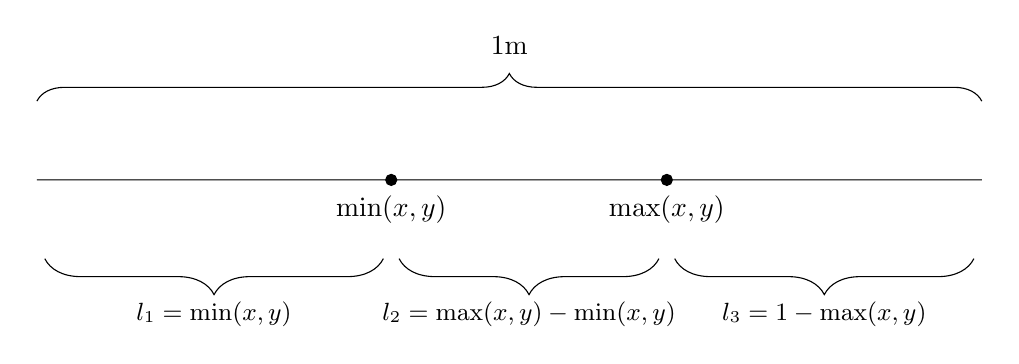
\begin{tikzpicture}
\draw[decorate, decoration={brace, amplitude=10pt}]
      (0,1) -- (12,1) node (A) [midway, yshift=20pt]{1m};
\filldraw
(0,0)
node[] (start) {}
--
(4.5,0)
circle (2pt)
node[below, yshift=-0.5ex]  {$\min(x,y)$}
--
(8,0)
circle (2pt)
node[below, yshift=-0.5ex] (y) {$\max(x,y)$} --
(12,0)
node[align=right,  below]
(end) {};
\draw[decorate, decoration={brace, mirror ,  amplitude=13pt}]
(0.1,-1) -- (4.4,-1)  node (A) [midway, align=center,  yshift=-20pt]{\small $l_1 = \min(x,y)$};
\draw[decorate, decoration={brace, mirror ,  amplitude=13pt}]
(4.6,-1) -- (7.9,-1)  node (A) [midway, yshift=-20pt]{\small $l_2 = \max(x,y)-\min(x,y)$};
\draw[decorate, decoration={brace, mirror ,  amplitude=13pt}]
(8.1,-1) -- (11.9,-1)  node (A) [midway, yshift=-20pt]{\small $l_3 = 1-\max(x,y)$};
\end{tikzpicture}
\end{center}
You know that the triangle can only be formed when the largest piece is less than the sum of the other two, but you have to express this as something that can be used algebraically.
Let
$l_\text{min}$,
$l_\text{mid}$, and
$l_\text{max}$
be the minimum, middle, and maximum values of
$(l_1, l_2, l_3)$.
Then
\begin{align*}
  l_\text{max} < l_\text{min} + l_\text{mid}
\end{align*}
and since
$  l_\text{min} + l_\text{mid} + l_\text{max}  = 1 $,
you have
\begin{align*}
  l_\text{max} < 1 - l_\text{max}  \\
2 l_\text{max} < 1 \\
 l_\text{max} < \frac{1}{2}
 \text{.}
\end{align*}
This is a necessary condition, and if
$\max(l_1, l_2, l_3)$
has to be less than
$\nicefrac{1}{2}$
then all three of
$l_1$, $l_2$, and $l_3$
must be less than $\nicefrac{1}{2}$.
Thus, you have to find
\begin{align*}
&\phantom{=}
P\left(
l_1 < \frac{1}{2} ,
l_2 < \frac{1}{2} ,
l_3 < \frac{1}{2}
\right)
\text{.}
\end{align*}
To evaluate this probability, integrate on the unit square to find the area where the crucial condition holds for any $(x,y)$ pair.
It is easier to consider the cases where $x<y$ and $x \geq y$ separately.
When $x<y$:
\begin{align*}
x     &< \frac{1}{2} \\
   y - x   &< \frac{1}{2} \\
1 -   y    &< \frac{1}{2}
\end{align*}
and you can find the area on the unit square where this holds.
\index{tricks!unit square integration}
Write these three conditions in the form $y < mx + c$,
\begin{align}
x  &< \frac{1}{2}     \label{eq:stickbreaking:line1}  \\
y  &< \frac{1}{2} + x \label{eq:stickbreaking:line2}  \\
y  &> \frac{1}{2}     \label{eq:stickbreaking:line3}
\text{,}
\end{align}
which can be plotted as lines on the unit square:
\begin{center}
\begin{tikzpicture}[scale=6, domain=0:1]
\draw (0,0)     --  (0,1) node[midway, left] {$y$}-- (1,1)  -- (1,0) -- (0,0) node[midway, below] {$x$};
\filldraw[pattern=dots, pattern color=lightgray] (0.5,0.5) -- (0.5,1) -- (0.0,0.5) -- (0.5,0.5);
\draw (0.5,0.5) -- (0.5,1) node[midway, right] {(\ref{eq:stickbreaking:line2})};
\draw (0,0.5)   -- (0.5,1) node[midway, above, sloped] {(\ref{eq:stickbreaking:line1})};
\draw (0.0,0.5) -- (0.5,0.5) node[midway, below] {(\ref{eq:stickbreaking:line3})};
\draw (0,0)     -- (1,1) node[midway, below, sloped]  {$y=x$} ;

\begin{scope}[xshift=1.4cm, yshift=-0.2cm, every node]

\draw[decorate, decoration={brace,  amplitude=13pt}] (0,1.08) -- (0.5,1.08) node [midway, yshift=+22pt]{$\frac{1}{2}$};
\draw[decorate, decoration={brace,  amplitude=13pt}] (-0.03,0.55) -- (-0.03,1.05) node [midway, xshift=-20pt]{$\frac{1}{2}$};

\filldraw[pattern=dots, pattern color=lightgray] (0.5,0.5) -- (0.5,1) -- (0.0,0.5) -- (0.5,0.5);
\filldraw[pattern=dots, pattern color=lightgray] (0,1.05) -- (0.5,1.05) -- (0.0,0.55) -- (0,1.05);

\end{scope}
\end{tikzpicture}
\end{center}
The area where all the conditions hold is the grey triangle.
When $y \leq x$, the region of interest will be mirrored in the line $y=x$.
The answer becomes the area of the square made up by the two triangles shown on the right, which is
$\frac{1}{2} \times \frac{1}{2} = \frac{1}{4}$, or exactly one quarter of the unit square.

This square is what \citet{JoshiQA} described in their answer.
When you need to integrate a bivariate uniform distribution on $[0,1]$, don't.
Instead, follow the advice in appendix \ref{ap:tricks} and draw a unit square and construct a shaded region in that square.
For this question, I would suggest knowing the method from \citet{JoshiQA}, in case the interviewer is looking for that answer, but be ready to work through it step by step as well.


% This line sets the tocdepth from here on forward
% Default is 2
\addtocontents{toc}{\protect\setcounter{tocdepth}{2}}

\section{Regression theory}
\label{sec:regressiontheory}
\index{regression theory}
The classic interview texts do not provide much information on regressions, but regression questions have become increasingly prevalent in recent years.
The first part in this section deals with multiple linear regression (the case where there are multiple explanatory variables), which is a generalisation of simple linear regression (only one explanatory variable).
For simple linear regression there are a few additional results that come in handy during interviews and it is worth looking over those.
After these two, I also provide some notes about logistic regression.
Linear and logistic regression make up the most prevalent models encountered not only in interviews, but also in practice.
In all cases, the Wikipedia articles are great overviews and I recommend reading them before interviews, in addition to this chapter.\\
\begin{itemize}
  \item \url{https://en.wikipedia.org/wiki/Linear_regression}
  \item \url{https://en.wikipedia.org/wiki/Simple_linear_regression}
  \item \url{https://en.wikipedia.org/wiki/Logistic_regression}
\end{itemize}

\subsection{Linear regression}
\index{regression theory!linear}
This is also known as multiple linear regression, to indicate that it uses multiple covariates.
Let $\beta$ be a matrix of parameters, and let $X$ be a vector of covariates.
For each observed $Y$, make the following assumption:
\[
  Y = X \beta + \varepsilon
  \text{.}
\]
Here, $Y$ is the variate, is $X$ the vector of covariates, and $\beta$ is the vector of parameters.

\subsubsection{Assumptions}
\begin{description}
  \item[Weak exogeneity:] the covariates are observed without error.
  \item[Linearity:] the mean of the variate is a linear combination of the parameters and the covariates.
  \item[Constant variance:] call it homoscedasticity for bonus points on terminology (in contrast to heteroscedasticity).
  This means that all the observations of $Y$ are assumed to have the same, constant variance.
  \item[Independence of errors:] we assume that the errors of the variates are uncorrelated.
  \item[No multicollinearity:] more properly, the lack of perfect multicollinearity. Assume that the covariates aren't perfectly correlated. See discussion below.
  \item[Errors have a statistical distribution:] this isn't strictly necessary, but it makes prediction theoretically coherent. The usual assumption is that the errors have a normal distribution, but others can also be used.
  (For instance, the t-distribution is used for ``robust regression'', where the variance observed is larger than that of the normal distribution.)
\end{description}



\subsubsection{If assumptions don't hold}


\begin{description}
  \item[Weak exogeneity:] the sensitivity of the model can be tested to the assumption of weak exogeneity by doing bootstrap sampling for the covariates and seeing how the sampling affects the parameter estimates.
  Covariates measured with error used to be a difficult problem to solve, as they required errors-in-variables models, which have very complicated likelihoods. In addition, there is no universal fitting library to deal with these. But nowadays, with the availability of Markov Chain Monte Carlo (MCMC) estimation through probabilistic programming languages, it is a lot easier to deal with these using Bayesian hierarchical models (or multilevel models, or Bayesian graphical models---these have many names).
  \item[Linearity:] the linear regression model only assumes linearity in the parameters, not the covariates. Therefore you could build a regression using non-linear transformations of the covariates, for instance,
  \[
    Y = X_1 \beta_1 +
        X_1^2 \beta_2 +
        \log(X_1) \beta_3
    \text{.}
  \]
  If you need to further relax the assumption, you are better off using non-linear modelling (see answer \ref{a:nameafewnonlinearmodels} for some examples).
  \item[Constant variance:] the simplest fix is to do a variance-stabilising transformation on the data. Assuming a constant coefficient of variation rather than a constant mean could also work. Some estimation libraries (such as the \verb+glm+ package in R) allow specifying the variance as a function of the mean.
  \item[Independence of errors:] this is dangerous because in the financial world things are usually highly correlated in times of crisis. The most important thing is to understand how risky this assumption is for your setting. If necessary, add a correlation structure to your model, or do  a multivariate regression. Both of these require significant resources to estimate parameters, not only in terms of computational power but also in the amount of data required.
  \item[No multicollinearity:] if the covariates are correlated, they can still be used in the regression, but numerical problems might occur depending on how the fitting algorithms invert the matrices involved.
  The t-tests that the regression produces can no longer be trusted. All the covariates must be included regardless of what their significance tests say.
  A big problem with multicollinearity, however, is over-fitting.
  Depending on how bad the situation is, the parameter values might have huge uncertainties around them, and if you fit the model using new data their values might change significantly.
  I suggest reading the Wikipedia article on multicollinearity, as it contains useful information: \\
  \url{https://en.wikipedia.org/wiki/Multicollinearity} \\
  Multicollinearity is a favourite topic of discussion for interviewers, and they usually have strong opinions about how it should be handled.
  The model's intended use will determine how sensitive it is to ignoring the error distribution.
  In many cases, fitting a line using least-squares estimation is equivalent to assuming errors have a normal distribution.
  If the real distribution has heavier tails, like the t-distribution, how risky will it make decisions based on your outputs?
  One way to address this is to use a technique like robust-regression.
  Another way is to think about the dynamics behind the problem and which distribution would be best suited to model them---as opposed to just fitting a curve through a set of points.
\end{description}

\subsubsection{Significance tests}
In the ordinary linear regression, the t-statistic is used to test the significance of each parameter,
\[
t_{\hat\beta}  =  \frac{\hat\beta - \beta_0}{ \text{stdev}( \tilde\beta) }
\]
where
${\text{stdev}( \tilde\beta)}$
is the standard deviation of the estimator
$\tilde\beta$.
For the classical linear regression with homoscedasticity and normal errors,
the sampling distribution of
$t_{\hat\beta}$
is the student's t-distribution with $(n-p)$ degrees of freedom.
Here, $\beta_0$ is a hypothesised value to test $\hat\beta$ against, usually set to $0$.

When multicollinearity is present, do not place too much emphasis on the interpretation of these statistics, as the  $\text{stdev}( \tilde\beta) $ will be high and the $\tilde\beta$ will be correlated. The t-statistic should not be confused with the Wald statistic, which is the equivalent test used in the case of logistic regression.

\subsubsection{Parameter estimation}
Since linear regressions are so well studied and prevalent in the literature, there exists a multitude of ways to estimate the parameters.
They can largely be grouped into the following:
\begin{description}
  \item[Least squares and related techniques.] This gives the well-known result
  \[
    \hat{\beta} = (X^T X)^{-1}X^T y
    \text{.}
  \]
  But inverting the matrix might be numerically troublesome in the case of high multicollinearity.
  Ordinary least squares implies the assumption of the normal distribution, and if you believe there is more variance in your data than the normal distribution can explain, you are better off using robust least-squares, or likelihood-based techniques along with the student's t-distribution.
  \item[Techniques based on the likelihood.]
  This necessitates assuming a statistical distribution on the data.
  To the frequentist, it then means maximising the likelihood.
  To the Bayesian, it means assuming a prior, multiplying it by the likelihood, and using the arising posterior distribution for inference.
\end{description}
Make sure you know some theory behind your favourite method and also know how to fit the linear regression using your favourite library without needing to Google.
Even better, know how to do this using both R and Python.
The section below provides a quick derivation of the least-squares result, followed by a section containing the derivation of the maximum likelihood estimate.


\subsubsection{Least squares}
\index{least squares}
\index{OLS|see {least squares}}
Assume you have $n$ rows in your dataset, and $p$ covariates.
Present the model in vectorised form:
\begin{align*}
Y = X \beta + \varepsilon
\text{,}
\end{align*}
where $\beta$ is a $(p \times 1)$ vector,
$X$ is an $n \times p$ matrix, and
$Y$ is an $n \times 1$ vector.
The errors can be written as
\begin{align*}
\varepsilon = Y-X \beta
\end{align*}
and you have the following total sum of squared errors,
\begin{align*}
S(\beta) &= \varepsilon^T \varepsilon \\
&= (Y-X\beta)^T (Y-X\beta)
\text{.}
\end{align*}
For the least-squared-error estimate, you want to find the $\beta$ that minimises the sum of squared errors. Take the derivative and set it equal to zero:
\begin{align*}
  S(\beta)
  &= Y^T Y -\beta^T X^T Y - Y^T X \beta + \beta^T X^T X \beta \\
  &= Y^T Y - 2 Y^T X \beta + \beta^T X^T X \beta
  & (\text{result is }n \times 1)
  \\
 \frac{\partial}{\partial\beta} S(\beta)
 &= - 2 X^T Y +
    2X^T X \beta
    & (\text{result is }p \times 1)
    \\
 \frac{\partial^2}{\partial\beta \partial\beta^T} S(\beta)
 &= 2
    X^T
    X
    & (\text{result is }p \times p)
    \text{.}
\end{align*}
The easiest way to convince yourself of the matrix derivatives is to work with $2 \times 2$ matrices.
Next, set the first derivative equal to zero to find a critical point of the function,
\begin{align*}
 \frac{\partial}{\partial\beta} S(\beta) &= 0 \\
  2X^T X \beta - 2 X^T Y &= 0 \\
  X^T X \beta &=  X^T Y  \\
   \beta &= (X^T X)^{-1} X^T Y
\end{align*}
giving the required result.
This is a minimum since the second derivative is a positive definite matrix.

\subsubsection{Likelihood}
\index{likelihood}
In order to use the likelihood, you need to make an assumption on the error.
If you assume the individual errors follow a normal distribution,
$\varepsilon_i \sim \text{Normal}(0, \sigma^2)$ for $ i = 1 ,2 , \ldots , n $,
then the error vector has a multivariate normal distribution, $\varepsilon \sim \text{MultivariateNormal}(\vec{0}, I_n \sigma^2)$,
where $I_n$ is the $n \times n$ identity matrix and $\sigma^2$ is the variance assumed on the errors. Using the same $X$, $Y$, and $\beta$ matrices as above, the linear model
\begin{align*}
  Y = X \beta + \varepsilon
\end{align*}
is equivalent to
\begin{align*}
  Y \sim \text{MultivariateNormal}(X \beta, I_n \sigma^2 )
  \text{.}
\end{align*}
The likelihood for this multivariate normal distribution is
\begin{align*}
\mathcal{L}(\theta;Y) &= f(Y) \\
&=
\frac{1}{\sqrt{(2\pi)^n \determinant{I_n \sigma^2} }}
\exp{
  \left(
  -\frac{1}{2}
   (Y-X\beta)^T  (I_n \sigma^2)^{-1} (Y - X \beta)
  \right)
} \\
&=
\frac{1}{\sqrt{(2\pi)^n  } \sigma^{n}}
\exp{
  \left(
  -\frac{1}{2 \sigma^2}
   (Y-X\beta)^T (Y-X\beta)
  \right)
}
\end{align*}
where $f(Y)$ is the pdf of the multivariate normal distribution.
The vector $\theta = \{ \beta, \sigma \}$ is the set of all parameters you want to estimate.
The maximum likelihood estimate (MLE) is the set of parameters that maximise the likelihood,
\begin{align}
\label{eq:regressiontheory:argmax}
\hat{\theta}_{\text{MLE}}
&=
\argmax_{\theta}
\mathcal{L}(\theta;Y)
\text{.}
\end{align}
Since the logarithm is a strictly increasing function, the likelihood and log likelihood will have a maximum at the same value of $\theta$,
which means either the likelihood or the log likelihood can be used, given that they will yield the same answer.
The log likelihood is more convenient to work with:
\begin{align*}
\log\mathcal{L}(\theta;Y)
&=
-\log\left(\sqrt{(2\pi)^n} \right)
-\log\sigma^{n}
  -\frac{1}{2 \sigma^2}
   (Y-X\beta)^T (Y-X\beta)
   \text{.}
\end{align*}
As with the least-squares derivation, you need to find a critical point.
Take the derivative with respect to the parameters of interest
\begin{align*}
 \frac{\partial}{\partial\beta}
\log\mathcal{L}(\theta;Y)
 &=
  \frac{1}{2 \sigma^2}
(  2 X^T Y -
    2X^T X \beta )
    \\
 \frac{\partial}{\partial\sigma}
\log\mathcal{L}(\theta;Y)
 &=
-\frac{n}{\sigma}
+  \frac{1}{\sigma^3}
   (Y-X\beta)^T (Y-X\beta)
   \text{,}
\end{align*}
which you set equal to zero
\begin{align*}
0
 &=
  \frac{1}{2 \sigma^2}
(  2 X^T Y -
    2X^T X \beta )
    \\
0
 &=
-\frac{n}{\sigma}
+  \frac{1}{\sigma^3}
   (Y-X\beta)^T (Y-X\beta)
   \text{,}
\end{align*}
and solving this system of equations yields the maximum likelihood estimates
\begin{align*}
\hat{\beta}_{\text{MLE}} &= (X^T X)^{-1} X^T Y
    \\
\hat{\sigma}_{\text{MLE}}
 &=
\sqrt{
\frac{1}{n}
   (Y-X\hat{\beta}_{\text{MLE}})^T (Y-X\hat{\beta}_{\text{MLE}})
   }
   \text{.}
\end{align*}
Check that these estimates do in fact maximise the log likelihood using the second order derivatives,
\begin{align*}
 \frac{\partial^2}{\partial\beta \partial\beta^T}
 \log\mathcal{L}(\theta;Y)
 &=
 - \frac{1}{ \sigma^2} X^T X
 \\
 \frac{\partial^2}{\partial\sigma^2}
\log\mathcal{L}(\theta;Y)
 &=
\frac{1}{\sigma^2}
\left(
 -\frac{3}{\sigma^2}
   (Y-X\beta)^T (Y-X\beta)
   + n
\right)
   \text{.}
\end{align*}
The first is
$ -\nicefrac{1}{ \sigma^2}$ multiplied by a positive definite matrix, which will be negative definite.
The second evaluates to
\[
-2n^2
\left(
  (Y-X\hat{\beta}_{\text{MLE}})^T
  (Y-X\hat{\beta}_{\text{MLE}})
\right)^{-1}
\]
when $\sigma = \hat{\sigma}_{\text{MLE}}$, which is also a negative quantity multiplied by a positive definite matrix.


Notice that the $\beta$ estimates are the same for least-squares estimation and maximum likelihood estimation.
This is only due to the assumption of the normal distribution and it will not hold in general for GLMs.
In addition, there will seldom be an analytical solution like the one presented.
For most GLMs you have to maximise the likelihood---or rather, the log likelihood---numerically, using an iterative approach like Newton's method, or similar.


\subsection{Simple linear regression}
\index{regression theory!simple linear}

The Simple linear regression is the special case of the linear regression with only one covariate
\[
  y = \alpha + x \beta
  \text{,}
\]
which is just a straight line fit.
Interviewers like this model for its aesthetically pleasing theoretical properties.
A few of them are described here, beginning with parameter estimation.
For $n$ pairs of $(x_i, y_i)$,
\[
  y_i = \alpha + \beta x_i + \varepsilon_i
\]
minimise the sum of squared errors,
\[
\sum_{i=1}^{n}{  \varepsilon_i^2 }
  =
\sum_{i=1}^{n}{ (y_i -  \alpha + \beta x_i)^2 }
\text{,}
\]
as before, but without matrices.
The least-squares estimators are:
\begin{align}
  \hat{\alpha} &= \bar{y} - \hat\beta \bar{x} \nonumber \\
  \hat{\beta} &=
  \frac
  {\sum_{i=1}^{n}{ (y_i - \bar{y}) (x_i - \bar{x}) }}
  {\sum_{i=1}^{n}{ (x_i - \bar{x})^2 }} \nonumber \\
  &=
  \frac
  {\Cov(x, y)}
  {\Var(x)} \label{eq:simple_linear_regression:var} \\
  &= \rho_{xy} \frac{s_y}{s_x} \label{eq:simple_linear_regression:corr}
  \text{.}
\end{align}
Use
\begin{align*}
\bar{y} &= \frac{1}{n}\sum_{i=1}^{n}{y_i} \\
\bar{x} &= \frac{1}{n}\sum_{i=1}^{n}{x_i}
\end{align*}
where $\Var$ and $\Cov$ are the variance and covariance, respectively.
Likewise,
$\rho_{xy}$,
$s_y$, and
$s_x$ are the sample correlation coefficient and sample standard deviations.
The final two lines of the equation,
(\ref{eq:simple_linear_regression:var})
and
(\ref{eq:simple_linear_regression:corr}),
are of utmost importance.
Learn them by heart, as they make many questions about simple linear regression much easier.
For example, ``when is the slope of a straight-line fit through a set of points $(x_i,y_i)$ equal to the correlation between $x$ and $y$?''

The final important result is that, for a simple linear regression, the $R^2$ value (which measures the proportion of variance in $y_i$ explained by the variance in $x_i$) is equal to the sample correlation coefficient squared,
\[
  R^2 = \rho_{yx}^2
  \text{.}
\]


\subsection{Logistic regression}
\index{regression theory!logistic}
Both the logistic regression and linear regression are GLMs, as introduced by \citet{GLM}, but users might spend years using regressions without ever encountering this term.
The techniques have different names in different fields, a phenomenon that has been made worse by the recent ``rediscovery'' of linear regression and logistic regression in Machine Learning.
It would be prudent to know some specialist theory and important results  about each of the three regressions discussed in this section, using the terminology that pertains to finance.

The assumptions for the logistic regression from the perspective of a GLM are identical to those of the linear regression, except that you are assuming linearity on the logit scale.
Let the variate of interest $y$ be a binary variable taking values of $0$ and $1$, then
\begin{align*}
y &\sim \text{Bernoulli}(p) \\
\text{logit}(p) &= X\beta  \quad (\text{logit link function})\\
\text{or}& \\
p &= \text{logistic}(X\beta)
\text{.}
\end{align*}
The only difference between the logistic and the probit regression is the link function.
For the probit regression you have
\begin{align*}
y &\sim \text{Bernoulli}(p) \\
\text{Probit}(p) &= X\beta  \quad (\text{Probit link function})\\
\text{or}& \\
p &= \Phi(X\beta)
\text{,}
\end{align*}
where $\Phi$ is the cumulative distribution function (CDF) of the standard normal distribution, and   $\text{Probit}(x)$ is the quantile function (or inverse CDF).\footnote{Notice that the naming convention isn't consistent, mostly due to historical reasons beyond the scope of this text.}
The R-square measure as defined for the linear regression doesn't exist for the logistic regression.
There are a few measures that act as pseudo R-squared, but I won't discuss them here---see the Wikipedia page for details.%
\footnote{\url{https://en.wikipedia.org/wiki/Logistic_regression\#Pseudo-R2s}}

\subsubsection{Significance tests}
Where the linear regression uses the t-statistic for significance testing, the logistic regression has the Wald-statistic. Asymptotically, it has a chi-squared distribution:
\[
W_{\hat\beta} =
\frac{(\hat\beta - \beta_0)^2}{ \text{stdev}( \tilde\beta) }
\sim \mathcal{X}^2
\]
where $\beta_0$ is a hypothesised value, as with the linear regression.



\subsubsection{Parameter estimation}

Similar to the linear regression, there are two schools of thought about parameter estimation for the logistic regression:
\begin{description}
  \item[Least squares and related techniques:]
    unlike the linear regression, you cannot get a closed-form solution and thus you have to use some sort of iterative method. Iteratively reweighted least squares are usually employed.
  \item[Techniques based on the likelihood:]
  a frequentist would need to maximise the likelihood using a numerical technique, whereas a Bayesian would evaluate the posterior distribution numerically, or sample from it using MCMC.
\end{description}



\section{Soft interview}

\subsection{Questions from them}

For more examples of soft interview questions (with suggested answers) see \citet{JoshiQA}.
Be ready to give some answers to the following questions:
\begin{itemize}
  \item Can you walk me through your CV?
  This is common, and is usually asked at the start of a phone interview.
  Rehearse an answer and try to keep it shorter than three minutes.
  It is vital to prepare a response and to tell it like a story.
  It looks bad if you can't articulate the contents of your CV.
  \item Why are you looking for a new job?
  I once had a phone interview where, upon answering the call, the guy immediately blurted ``Hi OK tell me why you want to leave your current job for one in finance?''
  He didn't even pause to tell me his name.
  You should have your answer to this question so well rehearsed that it sounds completely natural.
  \item Why do you want to work in finance?
  \item Why do you want to work for this firm and not our competitor?
\end{itemize}
%
Try not to start your sentences with ``So\ldots''.
It takes discipline to avoid, but it makes you sound more confident.
Also try and keep the number of filler words such as ``like'', ``umm'', and ``you know'' to a minimum.
You don't have to completely remove them to the point of sounding unnatural, but it is important to pay attention to how often you use them---especially under pressure.
This is most relevant to phone interviews, where your first impression is wholly determined by your eloquence.
Rehearse some answers to the questions above aloud.
Keep in mind that there may be a difference between your accent and that of the interviewer and adjust your tempo and enunciation accordingly.

\subsection{Questions for them}

At the end of every interview, interviewers usually ask if you have questions for them.
Have something to ask them.
If there are any obvious questions that come to light during the interviews, ask them.
I've seen interviewing guides online suggest questions like
``What is your greatest challenge over the coming months, and how will I be able to contribute to a solution?''
In my opinion this question feels rehearsed---don't bother with it.
Here are some questions you can ask, which are also relevant to the job:
\begin{itemize}
  \item Why is your team looking to hire at the moment? (Is it because of expansion, or to replace someone who recently left? This is important to know before accepting a position.)
  \item What operating systems do the team use?
  What are the proportions of Windows, Apple, GNU/Linux?
  \item  What does the team use for technical documentation? LaTeX, Wiki, Word, or nothing? (Don't say ``knowledge management'', you aren't interviewing to become a management consultant.)
  \item  What software does the team use for version control? Svn, Git, Mercurial, Team Foundation Server, or appending
  \verb+V1+,
  \verb+V2+,
  \verb+V3+
  to foldernames?
  \item  What programming languages does the team use? R, Python, C++, Julia, Matlab?
  For data analysis? For scripting? For production?
  \item  Is the team made up of Bayesians, frequentists, or whatever gets the job done?
  \item  What are the backgrounds of the other team members? What would someone with my background contribute?
  \item  Are modellers expected to write the code to implement their models, or is this handled by developers?
  \item  How are datasets accessed? SQL (Postgres, MySQL, MSSQL, sqlite), Hadoop, csvs, Excel, shared folders, or do people throw around USB sticks?
  \item  Are there formal mentor/mentee arrangements, or does this happen informally, or perhaps not at all?
  \item  Is there a formal process for requesting the installation of new software libraries?
  This is more R and Python specific, but it is important to ask if you expect to work with the latest technologies.
\end{itemize}
Even if you have asked these questions of some of the team members, ask them again and see whether you get the same answers.







\clearpage
\appendix

\phantomsection
\addcontentsline{toc}{section}{Appendix}
\section*{Appendix}

% This line sets the tocdepth from here on forward
% It means we hide subsections
\addtocontents{toc}{\protect\setcounter{tocdepth}{1}}

\section{Tricks}
\label{ap:tricks}
\index{tricks}
Here are some tricks I found useful while being brainteased.

\subsection{Start with simplest case}
\index{tricks!start with simplest case|textbf}
Start with the simplest case, and generalise eafter.
This often involves considering the case where $n=1$, then $2,3,4$, and so forth.
Though it feels simple it is not devoid of rigour, since it is often mandatory preparation for a proof by induction.
It is the most important trick of all.
During an interview, a never-before-seen brainteaser usually catches you by surprise and affects your ability to think clearly---especially since you have only 10 or 20 minutes to make an attempt.
When this happens the $n=1$ trick becomes a saviour.
Even if you don't manage to solve the problem you'll have shown the interviewer that you approach a difficult problem by breaking it down to its integral parts.
The best example of this appears in question
\ref{q:simplerandomwalkhittingprobability}.
Find further examples of this trick in questions
\ref{q:arraymissingnumber:a},
\ref{q:criminalsinfield},
and
\ref{q:bagnsockstwored}.

\subsection{Skip integration by drawing the unit square}
\index{tricks!unit square integration|textbf}
If a question involves two uniform distributions, chances are you can skip any integration by drawing a unit square and calculating areas on it.
More often than not this is also what the interviewer wants.
For examples of this, see the \emph{Stick Breaking} problem in section \ref{subsec:stickbreaking} and question \ref{q:romeojuliet}.
In both of these examples the integration would be cumbersome, but calculating the areas of triangles on the unit square is simple (if you correctly identify the areas of interest, that is).
The same idea is used in question \ref{q:rolltwodice} for a discreet sum.

\subsection{Recursion}
This is a trick I never encountered before I started interviewing.
It appears in section \ref{q:airforceone} with the \emph{Air Force One} question, as well as question \ref{q:simplerandomwalkhittingprobability}.
The idea is to express the answer you want as $P(A_n)$ or $p_n$ and then express $p_n$ in terms of $p_{n-1}$.
Then you can use recursion until you can solve for the quantity you want.
The same trick is sometimes used to calculate expectations of interest (using the Law of Total Expectation).
For a good example, see the question called ``Biased coins'' from \citet{WilmottFAQ}, and also the one called ``Two heads'' from the same book, which I reproduce here as a minimal-working example showing the method:

\begin{quote}
 When flipping an unbiased coin, how long do you have to wait on average before you get two heads in a row?
\end{quote}
I don't like the notation from Wilmott's answer since it is unclear whether his $N_n$ denotes an expectation or a probability, so I will amend it below.
Let $N_n$ be a random variable representing the number of coin flips you have to do to get $n$ heads in a row.
It satisfies the recursion relationship:
\begin{align*}
  N_n &=
  \overbrace{ \frac{1}{2} (N_{n-1} + 1)}^{n\text{th throw is heads}}
  +
  \overbrace{\frac{1}{2} (N_{n-1} + 1 + N_n)}^{n\text{th throw is tails}}
  \\
  \frac{1}{2}  N_n &=
   N_{n-1} + 1
  \\
  N_n &=
  2 N_{n-1} + 2
  \text{.}
\end{align*}
Wilmott solves for $N_n$, but that doesn't make sense if it is a random number.
Instead, you should solve for the expected value of $N_n$,
\begin{align*}
  E(N_n) &= 2 E(N_{n-1}) + 2
  \text{.}
\end{align*}
The expected number of throws to get heads once is $2$, so
$E(N_1) = 2$ (use the negative binomial distribution if you need to prove this),
\begin{align*}
  E(N_2) &= 2(2) + 2 = 6
  \text{.}
\end{align*}
This has the general solution of
\begin{align*}
  E(N_n) = 2^{n+1} - 2
\end{align*}
which you can prove using mathematical induction.
Questions that require martingale theory can often also be solved using the recursion technique, albeit with substantially more algebra (like question \ref{q:simplerandomwalkhittingprobability}).

\subsection{Central Limit Theorem}
\index{tricks!Central Limit Theorem|textbf}
Here the trick lies in identifying when a question is actually about the Central Limit Theorem.
I will not review the theory here, but make sure you understand the intuitive consequences:
if you sum a large number of random variables, the distribution of the sum approaches the normal distribution.\footnote{How many are required? Statisticians agree that 30 is large enough to be treated as infinity.}
For instance, here is a trick question:
\begin{quote}
You need 100 metres of wood.
One factory makes 100 metre pieces and another factory makes 1 metre pieces.
Both factories cite a 20\% error on their output.
Does it matter which factory you use?
\end{quote}
Note that the expected length of the end product is the same, and so is the variance.
The difference is the distribution.
You don't know what the error distribution of the $100m$ piece will be (the question doesn't tell you), but the sum of $1m$ pieces will have a distribution that is near normal.
If you worry about large outliers you probably prefer the normal distribution.
This is why insurers write millions of small policies rather than one big one.
Under some regularity conditions, their total loss will follow a normal distribution.
See question \ref{q:coin100flipsgamble} for the normal approximation to the binomial distribution, which is the same as the Central Limit Theorem applied to a sum of Bernoulli random variables.


\subsection{Normal distribution probabilities in your head}
\index{tricks!normal probabilities in your head|textbf}
A useful property of the normal distribution is that approximately 95\% of its mass lies within two standard deviations of the mean.
Some questions, like question \ref{q:coin100flipsgamble}, use this by having their quantities of interest lie two standard deviations from the mean.
The actual probability at this point is
\[
\Phi(2)
=  0.97725
\text{.}
\]
That is, if you have
$Z \sim \text{Normal}(0,1)$
then
$P(-2 <  Z \leq 2) = \Phi(2)- \Phi(-2) = 0.9545$.


\subsection{Law of Total Expectation}
\index{tricks!Law of Total Expectation|textbf}
Many brainteasers are interested in the expectation of some event, or the expected number of trials.
Thus, it is useful to know the Law of Total Expectation:
If $ A_1, A_2, A_3, \ldots, A_n$ are mutually disjoint and exhaustive, then
\[
  \E(Z) = \sum_{i=1}^{n}{
    \E(Z| A_i)P(A_i)
  }
  \text{.}
\]
For an example, see question \ref{q:bivariatenormalmax}.


\section{Code}
\subsection{Expectation of maximum of the bivariate normal distribution}
\label{ap:mvtnormproof}
Here is R code for a pseudo proof-by-simulation of question \ref{q:bivariatenormalmax}:

\inputminted{r}{./plots/mvtnorm/simtest.R}


\subsection{Why we need virtual functions}
\label{ap:virtualfunctions}
I produce my own take on the answer found at \\
\url{https://stackoverflow.com/questions/2391679/ddg#2392656}\\
Say you are working for the tax man, and you want to create a function that assigns the right tax rate to cars.
If you don't know the type of car, you will assume it burns fuel; make a class for generic cars and one for electric cars:
\inputminted{cpp}{./plots/virtualfunction/WithoutVirtual.cpp}
When you run this program, the output is:
\VerbatimInput{./plots/virtualfunction/WithoutVirtual.txt}
Oh no! The final line is incorrect, because you've accidentally treated the Tesla as a general car.
You would have to overload the \verb+queryEmssionsForTax+ function to take a
class of type
\verb+ElectricCar+.
But you don't want to burden the author of the
\verb+ElectricCar+
class with a list of external functions to maintain.
The solution is to use a virtual function.
Below, the only changes are to add
\verb+virtual+
to the function in the
\verb+Car+
class and
\verb+override+
to the function in the child class:
\inputminted{cpp}{./plots/virtualfunction/WithVirtual.cpp}
Now the output becomes:
\VerbatimInput{./plots/virtualfunction/WithVirtual.txt}

\subsection{SQL query practise script}
\label{ap:sqlite}
This script loads the tables and gives you the ability to test SQL queries.
I use the \verb+pandas+ and \verb+sqlite+ libraries, but you probably only need \verb+sqlite3+.
I also use Python since it is easy to install on most operating systems and it comes with sqlite functionality as standard.
\inputminted{python}{./plots/sql/sql.py}

\clearpage
\section{Crib sheet}
\label{ap:cribsheet}
Print this sheet and keep it with you during phone interviews, but make sure you are able to reproduce it wholly from memory at some point in your life.
Actual familiarity with the concepts is better than rote, but a combination of the two is required for good interview performance.


\begin{multicols}{2}

\subsection*{Miscellaneous}
ARMA(p, q):
\[
 Y_t = \alpha_0 +
 \underbrace{
  \sum_{i=1}^{p}{ \alpha_i Y_{t-i} }
  }_{\text{Autoregressive}}
  +
 \overbrace{
  \sum_{i=1}^{q}{ \beta_i \varepsilon_{t-i} }
  }^{\text{Moving average}}
  + \varepsilon_{t}
\]
\noindent
GARCH(p, q):
\begin{align*}
 Y_t &= \sigma_t Z_t  \quad \text{ where } Z_t \sim N(0,1) \\
 \sigma^2_{t}
 &=
 \alpha_0 +
  \sum_{i=1}^{p}{ \alpha_i Y^2_{t-i} }
  +
  \sum_{i=1}^{q}{ \beta_i \sigma^2_{t-i} }
\end{align*}


\begin{align*}
P(A_i|B)
&= \frac {P(B|A_i)P(A_i)} {P(B)} \\
&= \frac {P(B|A_i)P(A_i)} { \sum_{j} P(B|A_j)P(A_j) }
\end{align*}

\begin{align*}
{}_nC_{r} =
\binom{n}{k} &= \frac{n!}{ (n-k)! k! }
\end{align*}

\begin{align*}
  \sum_{k=0}^{n-1} {ar^k}    &= a \left(\frac{1-r^n}{1-r}\right) \\
  \sum_{k=0}^{\infty} {ar^k} &= \frac{a}{1-r} \text{ for } |r|<1
\end{align*}

\subsection*{Regression assumptions}

\begin{itemize}[itemsep=-2pt, topsep=2pt, partopsep=0pt]
  \small
  \item The covariates are observed without error (weak exogeneity)
  \item Linearity
  \item Constant variance (homoscedasticity)
  \item Independence of errors
  \item No (or very little) multicollinearity
  \item Statistical distribution, if required
\end{itemize}

\subsection*{Linear regression}
\[
    \hat{\beta} = (X^T X)^{-1}X^T y
\]

\[
t_{\hat\beta}  =  \frac{\hat\beta - \beta_0}{ \text{stdev}( \tilde\beta) } \sim t(v=n-p)
\]

\subsection*{Simple linear regression}
\begin{align*}
  \hat{\alpha} &= \bar{y} - \hat\beta \bar{x}  \\
  \hat{\beta} &=
  \frac
  {\sum_{i=1}^{n}{ (y_i - \bar{y}) (x_i - \bar{x}) }}
  {\sum_{i=1}^{n}{ (x_i - \bar{x})^2 }}  \\
  &=
  \frac
  {\Cov(x, y)}
  {\Var(x)} \\
  &= \rho_{xy} \frac{s_y}{s_x}
\end{align*}

\[
  R^2 = \rho_{yx}^2
\]

\subsection*{Logistic regression}
\[
W_{\hat\beta}
=  \frac{(\hat\beta - \beta_0)^2}{ \text{stdev}( \tilde\beta) }
\sim \mathcal{X}^2
\]


\subsection*{Calculus}
The following are important for most brainteasers:
\begin{itemize}
  \item
Product rule of differentiation:
\[
  \frac{d}{dx}
  g(x)f(x) =
  g'(x)f(x) +
  g(x)f'(x)
\]

  \item
Integration by parts:
\[
\int_{a}^{b}{ u dv }
=
uv\Big\vert_{x=a}^{x=b} - \int_{a}^{b}{ v du }
\]
  \item
Integration and differentiation rules involving $e^{x}$ and $\ln(x)$.
\end{itemize}


\end{multicols}
\clearpage




\phantomsection
\addcontentsline{toc}{section}{References}

\bibliography{books.bib}
%\bibliographystyle{plainnat}
\bibliographystyle{chicago}

\phantomsection
\addcontentsline{toc}{section}{Index}
\printindex

\end{document}

